\section{散射问题}
\subsection{球对称散射问题}
\subsubsection{电磁场按球坐标系展开}
\label{电磁场按球坐标展开}

定义角动量算符
\begin{equation*}
	\vb{L} = -i \vb{r} \times\nabla
\end{equation*}
易知
\begin{equation*}
	\vb{L} Y_{lm} = \sqrt{l(l+1)} \vb{X}_{lm}.
\end{equation*}

考虑电磁波在介电常量\(\varepsilon\)、磁导率\(\mu\)为常数的介质中传播，记介质阻抗为\(Z = \sqrt{\mu/\varepsilon}\)，电磁场按\(e^{-i\omega t}\)时谐因子振荡，\(k = \omega\sqrt{\mu\varepsilon}\)，以下\(\vb{E},\vb{H}\)代表略去时谐因子的振幅.

介质中的麦克斯韦方程为
\begin{equation*}
	\nabla \times \vb{E} = ikZ \vb{H},\quad \nabla \cdot \vb{E}=0,\quad \nabla \times \vb{H}=-\frac{ik}{Z}\vb{E},\quad \nabla \cdot \vb{H}=0.
\end{equation*}

以矢量球谐函数(VSH)为基展开
\begin{equation*}
	\begin{aligned}
		\vb{E} & = Z\sum_{l,m}\left( \frac{i}{k}a_{lm}\nabla\times\left(f_l(kr)\vb{X}_{lm}\right) + b_{lm}g_l(kr)\vb{X}_{lm} \right)                                                             \\
		       & = Z\sum_{l,m}\left( -\frac{a_{lm}\sqrt{l(l+1)}}{kr}f_l(kr)Y_{lm}\uv{r} + \frac{ia_{lm}}{kr}\frac{\d(rf_l(kr))}{\d r}\uv{r}\times\vb{X}_{lm} + b_{lm}g_l(kr)\vb{X}_{lm} \right). \\
		\vb{H} & = \sum_{l,m}\left( -\frac{i}{k}b_{lm}\nabla\times\left(g_l(kr)\vb{X}_{lm}\right) + a_{lm}f_l(kr)\vb{X}_{lm} \right)                                                             \\
		       & = \sum_{l,m}\left( -\frac{b_{lm}\sqrt{l(l+1)}}{kr}g_l(kr)Y_{lm}\uv{r} - \frac{ib_{lm}}{kr}\frac{\d(rg_l(kr))}{\d r}\uv{r}\times\vb{X}_{lm} + a_{lm}f_l(kr)\vb{X}_{lm} \right).
	\end{aligned}
\end{equation*}
其中，根据VSH的正交归一化性，也可以反解各项振幅得到
\begin{equation*}
	a_{lm}f_l(kr) &= \int\vb{H}\cdot\vb{X}_{lm}^*\d \Omega = -\frac{k}{Z\sqrt{l(l+1)}}\int\vb{r}\cdot\vb{E}Y_{lm}^*(\theta,\phi)\d \Omega.\\
	b_{lm}g_l(kr) &= \frac{1}{Z}\int\vb{E}\cdot\vb{X}_{lm}^*\d \Omega = \frac{k}{\sqrt{l(l+1)}}\int\vb{r}\cdot\vb{H}Y_{lm}^*(\theta,\phi)\d \Omega.
\end{equation*}

对于球对称体系，有限远处，能量辐射功率、电磁角动量辐射功率为：
\begin{equation*}
	\frac{\d P}{\d \Omega} &= \frac{r^2}{2}\uv{r}\cdot\Re\left[\vb{E}\times\vb{H}^*\right] \\
	&= \frac{r^2}{2}\sum_{l,l',m,m'}\Re\left[ Z\left( a_{lm}a_{l'm'}^*\frac{1}{ikr}\frac{\d(rf_l)}{\d r}f_{l'}^* + b_{lm}b_{l'm'}^*\left( \frac{1}{ikr}\frac{\d(rg_{l'})}{\d r} \right)^*g_l \right)\vb{X}_{lm}\cdot\vb{X}_{l'm'}^* \right. \\
		&\quad + \left. Z\left( a_{l'm'}^*b_{lm}g_lf_{l'}^* - a_{lm}b_{l'm'}^*\left( \frac{1}{ikr}\frac{\d(rg_{l'})}{\d r} \right)^*\frac{1}{ikr}\frac{\d(rf_l)}{\d r} \right)\vb{X}_{lm}\times\vb{X}_{l'm'}^*\cdot\uv{r} \right] .\\
	P &= \int\frac{\d P}{\d \Omega}\d \Omega = \frac{r^2}{2}\Re\left[ Z\sum_{l,m}\left( |a_{lm}|^2\frac{1}{ikr}\frac{\d(rf_l)}{\d r}f_l^* + |b_{lm}|^2\left( \frac{1}{ikr}\frac{\d(rg_l)}{\d r} \right)^*g_l \right) \right].\\
	\frac{\d^2\vb{L}}{\d t\,\d \Omega} &= \frac{r^3}{2}\Re\left[ \varepsilon(\vb{E}\times\uv{r})(\uv{r}\cdot\vb{E}^*)+\mu(\vb{H}\times\uv{r})(\uv{r}\cdot\vb{H}^*) \right]\\
	&= \frac{r^2}{2}\Re \sum_{l,l',m,m'}\frac{Z\sqrt{l'(l'+1)}Y_{l'm'}^*}{\omega}\Bigg[\left( a_{lm}a_{l'm'}^* + b_{lm}b_{l'm'}^* \right)\vb{X}_{lm}   \\
		&\quad + \left( a_{l'm'}^*b_{lm}\frac{1}{ikr}\frac{\d(rg_l)}{\d r}f_{l'}^* - a_{lm}b_{l'm'}^*\frac{1}{ikr}\frac{\d(rf_l)}{\d r}g_{l'}^* \right)\uv{r}\times\vb{X}_{lm}  \Bigg].
\end{equation*}

在远场辐射区域，上式可大幅度化简.取球贝塞尔函数解\(f_l(kr)=g_l(kr)=h_l^{(1)}(kr)\)，且\(\varepsilon=\varepsilon_0,\mu=\mu_0\)，\(Z=Z_0=\sqrt{\mu_0/\varepsilon_0}\)，\(k=k_0=\omega/c\)（\(k_0\)为实数，不考虑衰减）.

根据第一类球汉克尔函数的宗量渐进式
\begin{equation*}
	h_l^{(1)}(x)\sim\frac{1}{ix}\frac{\d(xh_l^{(1)}(x))}{\d x}\sim\frac{(-i)^{l+1}e^{ix}}{x},\quad x\gg1.
\end{equation*}
得到，在远场区域：
\begin{equation*}
	&\vb{E}_{sc} = \frac{Z_0e^{ik_0r}}{k_0r}\sum_{l,m}(-i)^{l+1}\left( -\frac{a_{lm}\sqrt{l(l+1)}}{k_0r}Y_{lm}\uv{r} - a_{lm}\uv{r}\times\vb{X}_{lm} + b_{lm}\vb{X}_{lm} \right).\\
	&\vb{H}_{sc} = \frac{e^{ik_0r}}{k_0r}\sum_{l,m}(-i)^{l+1}\left( \frac{b_{lm}\sqrt{l(l+1)}}{k_0r}Y_{lm}\uv{r} + b_{lm}\uv{r}\times\vb{X}_{lm} + a_{lm}\vb{X}_{lm} \right).\\
	&\frac{\d P_{sc}}{\d \Omega} = \frac{Z_0}{2k_0^2}\left| \sum_{l,m}\left( a_{lm}\vb{X}_{lm} + b_{lm}\uv{r}\times\vb{X}_{lm} \right) \right|^2,\quad P_{sc} = \frac{Z_0}{2k_0^2}\sum_{l,m}\left( |a_{lm}|^2 + |b_{lm}|^2 \right).\\
	&\frac{\d^2\vb{L}_{sc}}{\d t\d \Omega} = \frac{Z_0}{2k_0^2\omega}\Re\left[ \sum_{l,l',m,m'}\sqrt{l'(l'+1)}Y_{l'm'}^*i^{l'-l}\left( \left( a_{lm}a_{l'm'}^* + b_{lm}b_{l'm'}^* \right)\vb{X}_{lm} + \left( a_{l'm'}^*b_{lm} - a_{lm}b_{l'm'}^* \right)\uv{r}\times\vb{X}_{lm} \right) \right]\\
	&\frac{\d  \vb{L}_{sc}}{\d t}\cdot\uv{z}= \int\frac{\d^2\vb{L}_{\mathrm{sc}}}{\d t\d \Omega}\cdot\uv{z}\,\d \Omega = \frac{Z_0}{2k_0^2\omega}\sum_{l,m}m\left(|a_{lm}|^2 + |b_{lm}|^2\right).
\end{equation*}

\subsubsection{Mie 散射理论}
记入射平面电磁波 (下标 "inc") 的波矢沿 \(\uv{z}\)，则在 \(e^{-i\omega t}\) (假设散射体外为真空，波数为 \(k = \omega/c\)) 规范下，左旋光基矢为
\(\uv{e}_+ = (\uv{x} + i\uv{y})/\sqrt{2}\)，右旋光基矢为
\((\uv{x} - i\uv{y})/\sqrt{2}\)，则入射电磁场矢量总能写成形式：
\begin{equation*}
	\vb{E}_{\text{inc}} = E_{\text{inc}}\uv{e}_i e^{ikz}, \quad
	\vb{H}_{\text{inc}} = \frac{E_{\text{inc}}}{Z_0}\uv{z}\times\uv{e}_i e^{ikz}, \quad
	\uv{e}_i = A_+\uv{e}_+ + A_-\uv{e}_-, \quad |A_+|^2 + |A_-|^2 = 1.
\end{equation*}
其中 \(A_+,A_-\) 是常数，对于任意形式的入射偏振，左、右旋振幅可写作：
\begin{equation*}
	A_+ = \frac{1}{\sqrt{1 + \nu^2}},\quad A_- = \frac{\nu}{\sqrt{1 + \nu^2}}e^{i\psi}.
\end{equation*}

对于具有球对称性的散射体，以\(z\)轴为极轴建立球坐标系 \((r,\theta,\phi)\)，将平面波向球面波分解：
\begin{align*}
	\vb{E}_{\text{inc}} & = E_{\text{inc}}\uv{e}_i\sum_{l=0}^{\infty}i^l\sqrt{4\pi(2l+1)}j_l(kr)Y_{l0}(\theta),                         \\
	\vb{H}_{\text{inc}} & = \frac{E_{\text{inc}}}{Z_0}\uv{z}\times\uv{e}_i\sum_{l=0}^{\infty}i^l\sqrt{4\pi(2l+1)}j_l(kr)Y_{l0}(\theta).
\end{align*}

按照前述的方法展开，振幅系数
\begin{align*}
	a_{lm}f_l(kr) & = \int\vb{H}_{\text{inc}}\cdot\vb{X}_{lm}^*\d \Omega = i^{l-1}\sqrt{2\pi(2l+1)}(-A_-\delta_{m,-1}+A_+\delta_{m,1})\frac{E_{\text{inc}}}{Z_0}j_l(kr) = a_{l,\pm1}j_l(kr),         \\
	b_{lm}g_l(kr) & = \frac{1}{Z_0}\int\vb{E}_{\text{inc}}\cdot\vb{X}_{lm}^*\d \Omega = i^l\sqrt{2\pi(2l+1)}(A_-\delta_{m,-1}+A_+\delta_{m,1})\frac{E_{\text{inc}}}{Z_0}j_l(kr) = b_{l,\pm1}j_l(kr).
\end{align*}
进而，仅\(l\geq1,\,m=1\)的系数非零，对应
\begin{equation*}
	b_{l,1}=ia_{l,1}=i^l\sqrt{2\pi(2l+1)}\frac{A_-E_{\text{inc}}}{Z_0},\quad b_{l,-1}=-ia_{l,-1}=i^l\sqrt{2\pi(2l+1)}\frac{A_+E_{\text{inc}}}{Z_0}.
\end{equation*}

进而入射电磁场矢量可写作：
\begin{align*}
	\vb{E}_{\text{inc}} & = E_{\text{inc}}\sum_{l=1}^{\infty}i^l\sqrt{2\pi(2l+1)}A_{\pm}\left[j_l(kr)\vb{X}_{l,\pm1}\pm\frac{1}{k}\nabla\times\left(j_l(kr)\vb{X}_{l,\pm1}\right)\right],                   \\
	\vb{H}_{\text{inc}} & = \frac{E_{\text{inc}}}{Z_0}\sum_{l=1}^{\infty}i^{l-1}\sqrt{2\pi(2l+1)}A_{\pm}\left[\pm j_l(kr)\vb{X}_{l,\pm1}+\frac{1}{k}\nabla\times\left(j_l(kr)\vb{X}_{l,\pm1}\right)\right].
\end{align*}

在具体的散射问题中，根据自由空间与散射体的边界条件，可求出散射体内的电磁场 (int) 及散射电磁场 (sc)，其中，散射电磁场显然具有形式
\begin{align*}
	\vb{E}_{\text{sc}} & = E_{\text{inc}}\sum_{\pm}\sum_{l=1}^{\infty}i^l\sqrt{2\pi(2l+1)}A_{\pm}\left[\frac{\alpha_{l,\pm1}}{2}h_l^{(1)}(kr)\vb{X}_{l,\pm1}\pm\frac{1}{k}\nabla\times\left(\frac{\beta_{l,\pm1}}{2}h_l^{(1)}(kr)\vb{X}_{l,\pm1}\right)\right],                  \\
	\vb{H}_{\text{sc}} & = \frac{E_{\text{inc}}}{Z_0}\sum_{\pm}\sum_{l=1}^{\infty}i^{l-1}\sqrt{2\pi(2l+1)}A_{\pm}\left[\pm\frac{\beta_{l,\pm1}}{2}h_l^{(1)}(kr)\vb{X}_{l,\pm1}+\frac{1}{k}\nabla\times\left(\frac{\alpha_{l,\pm1}}{2}h_l^{(1)}(kr)\vb{X}_{l,\pm1}\right)\right].
\end{align*}

故散射体外部电磁场 (ext) 为
\(\vb{E}_{\text{ext}}=\vb{E}_{\text{sc}}+\vb{E}_{\text{inc}}\), \(\vb{H}_{\text{ext}}=\vb{H}_{\text{sc}}+\vb{H}_{\text{inc}}\).

记球对称散射体半径为\(R\)，则散射体的吸收功率为：
\begin{equation*}
	P_{\text{abs}} = \frac{R^2}{2}\int\Re\left[-\uv{r}\cdot\left(\vb{E}_{\text{ext}}\times\vb{H}_{\text{ext}}^*\right)\right]_{r=R}\d \Omega = \frac{\pi}{4k^2}\frac{E_{\text{inc}}^2}{Z_0}\sum_{\pm}\sum_{l=1}^{\infty}(2l+1)|A_{\pm}|^2\left(2-|1+\alpha_{l,\pm1}|^2-|1+\beta_{l,\pm1}|^2\right).
\end{equation*}
其中，根据球贝塞尔函数的数学性质，结果恰与\(R\)无关.

散射体的散射功率为：
\begin{align*}
	\frac{\d P_{\text{sc}}}{\d \Omega} & = \frac{r^2}{2}\uv{r}\cdot\Re\left[\vb{E}_{\text{sc}}\times\vb{H}_{\text{sc}}^*\right]_{kr\gg1}  = \frac{\pi}{4k^2}\frac{E_{\text{inc}}^2}{Z_0}\left|\sum_{\pm}\sum_{l=1}^{\infty}\sqrt{2l+1}A_{\pm}\left(\alpha_{l,\pm1}\vb{X}_{l,\pm1}\pm i\beta_{l,\pm1}\uv{r}\times\vb{X}_{l,\pm1}\right)\right|^2, \\
	P_{\text{sc}}                      & = \int\frac{\d P_{\text{sc}}}{\d \Omega}\d \Omega = \frac{\pi}{4k^2}\frac{E_{\text{inc}}^2}{Z_0}\sum_{\pm}\sum_{l=1}^{\infty}(2l+1)|A_{\pm}|^2\left(|\alpha_{l,\pm1}|^2+|\beta_{l,\pm1}|^2\right).
\end{align*}

系统对入射电磁波总的消耗功率为：
\begin{equation*}
	P_{\text{tot}}=P_{\text{abs}}+P_{\text{sc}}=-\frac{\pi}{2k^2}\frac{E_{\text{inc}}^2}{Z_0}\sum_{\pm}\sum_{l=1}^{\infty}(2l+1)|A_{\pm}|^2\left(\Re[\alpha_{l,\pm1}]+\Re[\beta_{l,\pm1}]\right).
\end{equation*}

入射能流为
\begin{equation*}
	\vb{S}_{\text{inc}}=\frac{1}{2}\Re\left(\vb{E}_{\text{inc}}\times\vb{H}_{\text{inc}}^*\right)=\frac{E_{\text{inc}}^2}{2Z_0}\uv{z}
\end{equation*}

对入射电场矢量做归一化处理，将以上各类功率除以入射能流，得各类散射截面为
\begin{align*}
	\sigma_{\text{abs}}                     & = \frac{\pi}{2k^2}\sum_{\pm}\sum_{l=1}^{\infty}(2l+1)|A_{\pm}|^2\left(2-|1+\alpha_{l,\pm1}|^2-|1+\beta_{l,\pm1}|^2\right),                                                 \\
	\frac{\d \sigma_{\text{sc}}}{\d \Omega} & = \frac{\pi}{2k^2}\left|\sum_{\pm}\sum_{l=1}^{\infty}\sqrt{2l+1}A_{\pm}\left(\alpha_{l,\pm1}\vb{X}_{l,\pm1}\pm i\beta_{l,\pm1}\uv{r}\times\vb{X}_{l,\pm1}\right)\right|^2, \\
	\sigma_{\text{sc}}                      & = \frac{\pi}{2k^2}\sum_{\pm}\sum_{l=1}^{\infty}(2l+1)|A_{\pm}|^2\left(|\alpha_{l,\pm1}|^2+|\beta_{l,\pm1}|^2\right),                                                       \\
	\sigma_{\text{tot}}                     & = -\frac{\pi}{k^2}\sum_{\pm}\sum_{l=1}^{\infty}(2l+1)|A_{\pm}|^2\Re\left(\alpha_{l,\pm1}+\beta_{l,\pm1}\right).
\end{align*}

\subsubsection{散射体实例}

\begin{example}
	半径为\(R\)，相对介电常数 \(\varepsilon_r\)，相对磁导率 \(\mu_r\) 的介质球

	记 \(n = \sqrt{\varepsilon_r\mu_r}\)，记\(k = \omega/c\).由于\(r\to0\) 处电磁场有限，应当取第一类贝塞尔函数\(j_l\)，设
	\begin{align*}
		\vb{E}_{\text{int}} & = E_{\text{inc}}\sum_{\pm}\sum_{l=1}^{\infty}i^l\sqrt{2\pi(2l+1)}A_{\pm}\left[c_{l,\pm1}j_l(nkr)\vb{X}_{l,\pm1}\pm\frac{d_{l,\pm1}}{nk}\nabla\times\left(j_l(nkr)\vb{X}_{l,\pm1}\right)\right],                                                     \\
		\vb{H}_{\text{int}} & = \frac{E_{\text{inc}}}{Z_0}\sqrt{\frac{\varepsilon_r}{\mu_r}}\sum_{\pm}\sum_{l=1}^{\infty}i^{l-1}\sqrt{2\pi(2l+1)}A_{\pm}\left[\pm d_{l,\pm1}j_l(nkr)\vb{X}_{l,\pm1}+\frac{c_{l,\pm1}}{nk}\nabla\times\left(j_l(nkr)\vb{X}_{l,\pm1}\right)\right].
	\end{align*}

	根据边界条件
	\begin{equation*}
		\varepsilon_r\uv{r}\cdot\vb{E}_{\text{int}}\big|_{R^-}=\uv{r}\cdot\vb{E}_{\text{ext}}\big|_{R^+}\quad\mu_r\uv{r}\cdot\vb{H}_{\text{int}}\big|_{R^-}=\uv{r}\cdot\vb{H}_{\text{ext}}\big|_{R^+}\quad\uv{r}\times\vb{E}_{\text{int}}\big|_{R^-}=\uv{r}\times\vb{E}_{\text{ext}}\big|_{R^+}\quad\uv{r}\times\vb{H}_{\text{int}}\big|_{R^-}=\uv{r}\times\vb{H}_{\text{ext}}\big|_{R^+}
	\end{equation*}

	得
	\begin{align*}
		 & j_l(kR)+\frac{\alpha_{l,\pm1}}{2}h_l^{(1)}(kR) = c_{l,\pm1}j_l(nkR), \quad j_l(kR)+\frac{\beta_{l,\pm1}}{2}h_l^{(1)}(kR) = \frac{n}{\mu_r}d_{l,\pm1}j_l(nkR),                            \\
		 & \frac{\d(krj_l(kr))}{\d(kr)}\bigg|_{r=R}-\frac{\beta_{l,\pm1}}{2}\frac{\d(krh_l^{(1)}(kr))}{\d(kr)}\bigg|_{r=R} = \frac{1}{n}d_{l,\pm1}\frac{\d(nkrj_l(nkr))}{\d(nkr)}\bigg|_{r=R},      \\
		 & \frac{\d(krj_l(kr))}{\d(kr)}\bigg|_{r=R}+\frac{\alpha_{l,\pm1}}{2}\frac{\d(krh_l^{(1)}(kr))}{\d(kr)}\bigg|_{r=R} = \frac{1}{\mu_r}c_{l,\pm1}\frac{\d(nkrj_l(nkr))}{\d(nkr)}\bigg|_{r=R}.
	\end{align*}
	解得
	\begin{align*}
		c_{l,\pm1}      & = \frac{\mu_r\left(J_lH_l'-H_lJ_l'\right)}{\mu_rH_l'\Pi_l-H_l\Pi_l'}, \quad d_{l,\pm1} = \frac{n\left(J_lH_l'-H_lJ_l'\right)}{\varepsilon_r\Pi_lH_l'-H_l\Pi_l'},                                       \\
		\alpha_{l,\pm1} & = 2\frac{J_l\Pi_l'-\mu_r\Pi_lJ_l'}{\mu_rH_l'\Pi_l-H_l\Pi_l'}=e^{i2\delta_{l}}-1, \quad \beta_{l,\pm1} = 2\frac{J_l\Pi_l'-\varepsilon_r\Pi_lJ_l'}{\varepsilon_r\Pi_lH_l'-H_l\Pi_l'}=e^{i2\Delta_{l}}-1.
	\end{align*}
	其中
	\begin{equation*}
		&J_l = j_l(kR),\quad N_l = n_l(kR),\quad \Pi_l = j_l(nkR),\quad H_l = J_l + iN_l.\\
		&J_l' = \left.\frac{\d(krj_l(kr))}{\d(kr)}\right|_{r=R},\quad
		N_l' = \left.\frac{\d(krn_l(kr))}{\d(kr)}\right|_{r=R},\quad
		\Pi_l' = \left.\frac{\d(nkrj_l(nkr))}{\d(nkr)}\right|_{r=R},\quad
		H_l' = J_l' + iN_l'.\\
		&\delta_{l} = \arctan\left(\frac{J_l\Pi_l' - \mu_r\Pi_lJ_l'}{N_l\Pi_l' - \mu_r\Pi_lN_l'}\right),\quad
		\Delta_{l} = \arctan\left(\frac{J_l\Pi_l' - \varepsilon_r\Pi_lJ_l'}{N_l\Pi_l' - \varepsilon_r\Pi_lN_l'}\right).
	\end{equation*}

	各类散射面积为
	\begin{equation*}
		\sigma_{\text{abs}}=0\quad \sigma_{\text{tot}}=\sigma_{\text{sc}}=\frac{2\pi}{k^2}\sum_{l=1}^{\infty}(2l+1)\left(\sin^2\delta_{l}+\sin^2\Delta_{l}\right)
	\end{equation*}


	当散射体很小（长波长散射）或很大(短波长散射)时，振幅可近似为(记\(z_r=\sqrt{\mu_r/\varepsilon_r}\))：
	\begin{equation*}
		\alpha_{l,\pm1}=
		\begin{cases}
			\displaystyle
			\frac{2 i \,(\mu_r-1)(l+1)\,(kR)^{2l+1}}
			{\big(\mu_r l+l+1\big)\,(2l+1)!!\,(2l-1)!!},
			 & kR\ll 1, \\[6pt]
			\displaystyle
			-1+(-1)^l\exp\!\left(-2 i\,kR+\arctan\!\Big(z_r\tan\!\big(nkR-\frac{l\pi}{2}\big)\Big)\right),
			 & kR\gg 1,
		\end{cases}
	\end{equation*}
	\begin{equation*}
		\beta_{l,\pm1}=
		\begin{cases}
			\displaystyle
			\frac{2 i \,(\varepsilon_r-1)(l+1)\,(kR)^{2l+1}}
			{\big(\varepsilon_r l+l+1\big)\,(2l+1)!!\,(2l-1)!!},
			 & kR\ll 1, \\[6pt]
			\displaystyle
			-1+(-1)^l\exp\!\left(-2 i\,kR+\arctan\!\Big(\frac{1}{z_r}\tan\!\big(nkR-\frac{l\pi}{2}\big)\Big)\right),
			 & kR\gg 1.
		\end{cases}
	\end{equation*}
\end{example}

\begin{example}
	半径为\(R\)，表面相对阻抗为\(z_s\)的球

	根据表面相对阻抗定义 \begin{equation*}
		\uv{r} \times \left( \vb{E}_\text{ext}\big|_{R} \times \uv{r} \right) = \frac{z_s}{Z_0} \uv{r} \times \vb{H}_\text{ext}\big|_{R}
	\end{equation*}
	得
	\begin{align*}
		j_l(kR)+\frac{\alpha_{l,\pm1}}{2}h_l^{(1)}(kR) & = i\frac{z_s}{kR}\frac{\d(kr(j_l(kr)+\frac{\alpha_{l,\pm1}}{2}h_l^{(1)}(kr)))}{\d(kr)}\bigg|_{r=R},     \\
		j_l(kR)+\frac{\beta_{l,\pm1}}{2}h_l^{(1)}(kR)  & = i\frac{z_s^{-1}}{kR}\frac{\d(kr(j_l(kr)+\frac{\beta_{l,\pm1}}{2}h_l^{(1)}(kr)))}{\d(kr)}\bigg|_{r=R}.
	\end{align*}

	解得
	\begin{equation*}
		\alpha_{l,\pm1} = -1-\frac{H_l^*kR-iz_sH_l'^*}{H_lkR-iz_sH_l'}, \quad \beta_{l,\pm1} = -1-\frac{H_l^*kR-iz_s^{-1}H_l'^*}{H_lkR-iz_s^{-1}H_l'}.
	\end{equation*}

	对于 \(z_s\to0\) 或 \(\infty\)，及 \(\Re(z_s)=0\) 三类情况，振幅可化简为：
	\begin{equation*}
		\alpha_{l,\pm1}=-1+e^{2i\delta_{l}},\quad \beta_{l,\pm1}=-1+e^{2i\Delta_{l}}
	\end{equation*}
	其中
	\begin{equation*}
		\tan\delta_{l}=
		\begin{cases}
			J_l/N_l,                                    & z_s\to0,      \\
			J_l'/N_l',                                  & z_s\to\infty, \\
			\dfrac{J_l+\Im(z_s)J_l'}{N_l+\Im(z_s)N_l'}, & \Re(z_s)=0.
		\end{cases}\quad
		\tan\Delta_{l}=
		\begin{cases}
			J_l'/N_l',                                            & z_s\to0,      \\
			J_l/N_l,                                              & z_s\to\infty, \\
			\dfrac{J_l+\Im(z_s^{-1})J_l'}{N_l+\Im(z_s^{-1})N_l'}, & \Re(z_s)=0.
		\end{cases}
	\end{equation*}

	当散射体很小（长波长散射）或很大(短波长散射)时，振幅可近似为：
	\begin{equation*}
		\alpha_{l,\pm1}&=
		\begin{cases}
			-\dfrac{2i(kR)^{2l+1}}{[(2l+1)(2l-1)!!]^2}\dfrac{kR-i z_s(l+1)}{kR+i z_s l}, & kR\ll1, \\
			\dfrac{z_s-1}{z_s+1}(-1)^{l+1}e^{-2ikR}-1,                                   & kR\gg1.
		\end{cases}\\
		\beta_{l,\pm1}&=
		\begin{cases}
			-\dfrac{2i(kR)^{2l+1}}{[(2l+1)(2l-1)!!]^2}\dfrac{kR-i z_s^{-1}(l+1)}{kR+i z_s^{-1}l}, & kR\ll1, \\
			\dfrac{z_s-1}{z_s+1}(-1)^l e^{-2ikR}-1,                                               & kR\gg1.
		\end{cases}
	\end{equation*}

	注意，相对介电常数 \(\varepsilon_r\)，相对磁导率 \(\mu_r\) 的介质球无法引入表面相对阻抗，不能按此法处理.
\end{example}

\begin{example}
	长波长散射\(kR\ll1\)

	可保留至最低阶  \(l = 1\) 项，记
	\(\alpha_{\pm} = \alpha_{1,\pm1}\)，\(\beta_{\pm} = \beta_{1,\pm1}\)，远场各项为
	\begin{align*}
		\vb{E}_{\rm sc} & = \sqrt{\dfrac{3 \pi}{2}} E_{\rm inc} \dfrac{e^{ikr}}{kr} \sum\limits_{\pm}
		A_{\pm}\bigl(\pm \beta_{\pm}\uv{r}\times\vb{X}_{1,\pm1} -
		i\alpha_{\pm}\vb{X}_{1,\pm1}\bigr),\quad \vb{H}_{\rm sc}=\frac{1}{Z_0}\uv{n}_s\times\vb{E}_{\rm sc}                                                                                                      \\
		\frac{\d \sigma_{\mathrm{sc}}}{\d \Omega}
		                & = \frac{9}{32k^2}\!\left[(1+\cos^2\theta)\left(|A_+|^2(|\alpha_+|^2+|\beta_+|^2)+|A_-|^2(|\alpha_-|^2+|\beta_-|^2)\right)\right.                                                       \\
		                & \quad\left. +2\sin^2\theta\Re\left(A_+A_-^*(\alpha_+\alpha_-^*-\beta_+\beta_-^*)e^{i2\phi}\right)+4\cos\theta\Re\left(|A_+|^2\alpha_+\beta_+^*+|A_-|^2\alpha_-\beta_-^*\right)\right], \\
		\sigma_{\mathrm{sc}}
		                & = \frac{3\pi}{2k^2}\left(|A_+|^2(|\alpha_+|^2+|\beta_+|^2)+|A_-|^2(|\alpha_-|^2+|\beta_-|^2)\right),                                                                                   \\
		\sigma_{\mathrm{abs}}
		                & = \frac{3\pi}{2k^2}\left(|A_+|^2(2-|1+\alpha_+|^2-|1+\beta_+|^2)+|A_-|^2(2-|1+\alpha_-|^2-|1+\beta_-|^2)\right),                                                                       \\
		\sigma_{\mathrm{tot}}
		                & = \sigma_{\mathrm{abs}}+\sigma_{\mathrm{sc}}=-\frac{3\pi}{k^2}\Re\left(|A_+|^2(\alpha_++\beta_+)+|A_-|^2(\alpha_-+\beta_-)\right).
	\end{align*}

	在大多情况下，正负散射振幅相等，即
	\(\alpha_{\pm} = \alpha\)，\(\beta_{\pm} = \beta\)，此时注意到
	\begin{equation*}
		\vb{X}_{1,\pm1} &= \sqrt{\dfrac{3}{8 \pi}} \bigl(\cos\theta \uv{e}_{\pm} -
		\dfrac{1}{\sqrt{2}} \sin\theta e^{\pm i\phi}\uv{z}\bigr),\\
		\uv{r}\times\vb{X}_{1,\pm1} &= \pm i \sqrt{\dfrac{3}{32 \pi}} \Bigl[-(1+\cos^2\theta)\uv{e}_{\pm} + \sin^2\theta e^{\pm 2i\phi}\uv{e}_{\mp} +
			\sqrt{2} \sin\theta \cos\theta e^{\pm i\phi}\uv{z}\Bigr].
	\end{equation*}

	代入入射偏振方向、入射方向、散射方向
	\begin{equation*}
		\uv{e}_i = A_+\uv{e}_+ + A_-\uv{e}_-,\quad \uv{n}_i = \uv{z},\quad\uv{n}_s = \uv{r}.
	\end{equation*}

	不难得到
	\begin{equation*}
		(\uv{n}_s\times\uv{e}_i)\times\uv{n}_s &= -\dfrac{\sin\theta \cos\theta}{\sqrt{2}}\bigl(e^{-i\phi}A_- + e^{i\phi}A_+\bigr)\uv{z} +
		\dfrac{(1+\cos^2\theta)A_+ - A_-e^{-2i\phi}}{2}\uv{e}_+ + \dfrac{(1+\cos^2\theta)A_- - A_+e^{2i\phi}}{2}\uv{e}_- \\&=
		\sqrt{\dfrac{8 \pi}{3}}i\bigl(A_+\uv{r}\times\vb{X}_{1,1} - A_-\uv{r}\times\vb{X}_{1,-1}\bigr)\\
		(\uv{n}_i\times\uv{e}_i)\times\uv{n}_s &= -\dfrac{\sin\theta}{\sqrt{2}}\bigl(e^{-i\phi}A_- + e^{i\phi}A_+\bigr)\uv{z} + A_+\cos\theta \uv{e}_+ + A_-\cos\theta \uv{e}_-\\&=
		\sqrt{\dfrac{8 \pi}{3}}\bigl(A_+\vb{X}_{1,1} + A_-\vb{X}_{1,-1}\bigr).
	\end{equation*}

	故
	\begin{equation*}
		\vb{E}_{\rm sc} = -\dfrac{3}{4}i E_{\rm inc} \dfrac{e^{ikr}}{kr}\bigl(\alpha(\uv{n}_s\times\uv{e}_i)\times\uv{n}_s + \beta(\uv{n}_i\times\uv{e}_i)\times\uv{n}_s\bigr) = \dfrac{k^2 e^{ikr}}{4 \pi\varepsilon_0} E_{\rm inc}\bigl(\kappa_e (\uv{n}_s\times\uv{e}_i)\times\uv{n}_s +
		\kappa_m (\uv{n}_i\times\uv{e}_i)\times\uv{n}_s\bigr).
	\end{equation*}
	其中
	\begin{equation*}
		\kappa_e = \dfrac{3 \pi\varepsilon_0}{i k^3}\alpha, \quad \kappa_m = \dfrac{3 \pi\varepsilon_0}{i k^3}\beta.
	\end{equation*}

	这说明，长波长散射最低阶由诱导电偶极矩、磁偶极矩贡献，其大小为
	\begin{equation*}
		\vb{p} = \kappa_e \vb{E}_{\rm inc},\quad
		\vb{m} = \kappa_m c^2 \mu_0 \vb{H}_{\rm inc} = c\kappa_m \uv{n}_i\times\vb{E}_{\rm inc}
	\end{equation*}
	而其它截面项则化简为
	\begin{align*}
		\frac{\d \sigma_{\mathrm{sc}}}{\d \Omega}
		                 & = \frac{9}{32k^2}\!\left[(1+\cos^2\theta)(|\alpha|^2+|\beta|^2) + 2\sin^2\theta(|\alpha|^2-|\beta|^2)\Re\left(A_+A_-^*e^{i2\phi}\right) + 4\cos\theta\Re(\alpha\beta^*)\right] \\
		                 & = \dfrac{k^4}{16 \pi^2 \varepsilon_0^2}\bigl|\kappa_e (\uv{n}_s\times\uv{e}_i)\times\uv{n}_s - \kappa_m (\uv{n}_i\times\uv{e}_i)\times\uv{n}_s\bigr|^2.                        \\
		\sigma_{\mathrm{sc}}
		                 & = \frac{3\pi}{2k^2}(|\alpha|^2+|\beta|^2)=\dfrac{k^4}{6 \pi \varepsilon_0^2}\bigl(|\kappa_m|^2+|\kappa_e|^2\bigr)                                                              \\
		\sigma_{\rm tot} & = -\dfrac{3 \pi}{k^2}\Re\bigl(\alpha+\beta\bigr) = \dfrac{k}{\varepsilon_0}\Im\bigl(\kappa_e+\kappa_m\bigr),\quad
		\sigma_{\rm abs} = \sigma_{\rm tot} - \sigma_{sc}.
	\end{align*}

	比如，椭圆偏振光入射介质球
	\begin{equation*}
		A_+ = \dfrac{1}{\sqrt{1+\nu^2}}, \quad A_- = \dfrac{\nu}{\sqrt{1+\nu^2}}e^{i\psi}.
	\end{equation*}

	可以通过前部分的结论取极限得
	\begin{equation*}
		\alpha &= \alpha_{1,\pm1} = \exp\Bigl[2i\arctan\Bigl(\dfrac{J_1\Pi_1'- \mu_r \Pi_1 J_1'}{N_1\Pi_1'- \mu_r \Pi_1 N_1'}\Bigr)\Bigr]_{kR\ll1}-1 = i\dfrac{4}{3}\dfrac{\mu_r-1}{\mu_r+2}(kR)^3,\\
		\beta &= \beta_{1,\pm1} = \exp\Bigl[2i\arctan\Bigl(\dfrac{J_1\Pi_1'- \mu_r \Pi_1 J_1'}{N_1\Pi_1'- \varepsilon_r \Pi_1 N_1'}\Bigr)\Bigr]_{kR\ll1}-1 = i\dfrac{4}{3}\dfrac{\varepsilon_r-1}{\varepsilon_r+2}(kR)^3.
	\end{equation*}

	或者根据电磁学经典的结论得
	\begin{equation*}
		\kappa_m = 4\pi \varepsilon_0 R^3 \dfrac{\varepsilon_r-1}{\varepsilon_r+2}, \quad \kappa_e = 4\pi \varepsilon_0 R^3 \dfrac{\mu_r-1}{\mu_r+2} \quad\implies\quad
		\alpha = i\dfrac{4}{3}\dfrac{\mu_r-1}{\mu_r+2}(kR)^3, \quad \beta = i\dfrac{4}{3}\dfrac{\varepsilon_r-1}{\varepsilon_r+2}(kR)^3.
	\end{equation*}

	进而散射截面为
	\begin{align*}
		\frac{\d \sigma_{\text{sc}}}{\d \Omega} & = \frac{R^6k^4}{2}\left[(1+\cos^2\theta)\left(\left|\frac{\varepsilon_r-1}{\varepsilon_r+2}\right|^2+\left|\frac{\mu_r-1}{\mu_r+2}\right|^2\right)+2\sin^2\theta\frac{\nu}{1+\nu^2}\cos(\psi-2\phi)\left(-\left|\frac{\varepsilon_r-1}{\varepsilon_r+2}\right|^2+\left|\frac{\mu_r-1}{\mu_r+2}\right|^2\right)\right. \\
		                                        & \quad\left.+4\cos\theta\,\Re\left(\frac{\mu_r-1}{\mu_r+2}\left(\frac{\varepsilon_r-1}{\varepsilon_r+2}\right)^*\right)\right],                                                                                                                                                                                        \\
		\sigma_{\text{sc}}                      & = \frac{8\pi}{3}R^6k^4\left(\left|\frac{\varepsilon_r-1}{\varepsilon_r+2}\right|^2+\left|\frac{\mu_r-1}{\mu_r+2}\right|^2\right).
	\end{align*}

	若 \(\nu=1,\psi=2\chi\)，即入射电磁波是偏振方向与 \(\uv{x}\) 夹角为 \(\chi\) 的线偏振光，得
	\begin{equation*}
		\frac{\d \sigma_{\text{sc}}}{\d \Omega}\bigg|_{\nu=1,\psi=2\chi}=R^6k^4\left[\cos^2(\chi-\phi)\left|\frac{\varepsilon_r-1}{\varepsilon_r+2}\cos\theta+\frac{\mu_r-1}{\mu_r+2}\right|^2+\sin^2(\chi-\phi)\left|\frac{\varepsilon_r-1}{\varepsilon_r+2}+\frac{\mu_r-1}{\mu_r+2}\cos\theta\right|^2\right].
	\end{equation*}

	若 \(\varepsilon_r\gg1,\mu_r=1\)，即对于易极化的非磁性球体，得
	\begin{equation*}
		\frac{\d \sigma_{\text{sc}}}{\d \Omega}\bigg|_{\varepsilon_r\gg1,\mu_r=1} = \frac{R^6k^4}{2}\left[(1+\cos^2\theta)-2\sin^2\theta\frac{\nu}{1+\nu^2}\cos(\psi-2\phi)\right],\quad
		\sigma_{\text{sc}} = \frac{8\pi}{3}R^6k^4.
	\end{equation*}

	比如，椭圆偏振光入射趋肤深度为 \(\delta_c=\sqrt{2/\omega\mu_c\sigma_c}\ll R\) 的良导体球，其表面相对阻抗为 \(z_s=k\delta_c(1-i)/2\)，代入振幅近似公式，并注意到 \(kR\ll1\) 得：
	\begin{equation*}
		\alpha=\alpha_{1,\pm1}=-\frac{2i}{3}(kR)^3\left(1-\frac{3}{2}(1+i)\frac{\delta_c}{R}\right) ,\quad\beta=\beta_{1,\pm1}=\frac{4i}{3}(kR)^3
	\end{equation*}

	进而散射功率、吸收功率、总消耗功率为
	\begin{equation*}
		\frac{\d \sigma_{\text{sc}}}{\d \Omega}&=\frac{R^6k^4}{8}\left[5(1+\cos^2\theta)\left(1-\frac{3\delta_c}{5R}\right)-6\sin^2\theta\frac{\nu}{1+\nu^2}\cos(\psi-2\phi)\left(1+\frac{\delta_c}{R}\right)-8\cos\theta\left(1-\frac{3\delta_c}{2R}\right)\right]\\
		\sigma_{\text{sc}}&=\frac{10\pi R^6k^4}{3}\left(1-\frac{3\delta_c}{5R}\right)\ll\sigma_{\text{abs}}=\sigma_{\text{tot}}=3\pi kR^2\delta_c
	\end{equation*}
\end{example}

\subsection{无限长圆柱散射问题}

\subsubsection{柱坐标下Helmholtz方程的解}

在球体散射的基础上，来看柱体的散射。柱坐标下，Helmholtz型方程
\begin{equation*}
	(\nabla^2 + k^2)\vb{f} = 0
\end{equation*}
的解总可以分解为
\begin{align*}
	\vb{f}      & = \sum_{m=-\infty}^{\infty} \sum_n \bigl(a_{mn}\vb{M}_{mn} + b_{mn}\vb{N}_{mn} + c_{mn}\vb{L}_{mn}\bigr),                                                                                                                     \\
	\vb{L}_{mn} & = \frac{1}{k} \nabla \bigl(Z_m(k_{\perp n} \rho) e^{im\phi + ik_{z,n}z}\bigr)                                                                                                                                                 \\
	            & = \left( \frac{ik_{z,n}}{k} Z_m(k_{\perp n} \rho) \uv{z} + \frac{k_{\perp n}}{k} Z_m'(k_{\perp n} \rho) \uv{\rho} + \frac{im}{k\rho} Z_m(k_{\perp n} \rho) \uv{\phi} \right) e^{im\phi + ik_{z,n}z},                          \\
	\vb{M}_{mn} & = \frac{1}{k} \nabla \times \bigl(\uv{z} Z_m(k_{\perp n} \rho) e^{im\phi + ik_{z,n}z}\bigr)                                                                                                                                   \\
	            & = \left( \frac{im}{k\rho} Z_m(k_{\perp n} \rho) \uv{\rho} - \frac{k_{\perp n}}{k} Z_m'(k_{\perp n} \rho) \uv{\phi} \right) e^{im\phi + ik_{z,n}z},                                                                            \\
	\vb{N}_{mn} & = \frac{1}{k} \nabla \times \vb{M}_{mn}                                                                                                                                                                                       \\
	            & = \left( \frac{k_{\perp n}^2}{k^2} Z_m(k_{\perp n} \rho) \uv{z} + \frac{ik_{z,n}k_{\perp n}}{k^2} Z_m'(k_{\perp n} \rho) \uv{\rho} - \frac{mk_{z,n}}{k^2\rho} Z_m(k_{\perp n} \rho) \uv{\phi} \right) e^{im\phi + ik_{z,n}z}.
\end{align*}
其中
\begin{equation*}
	k_{\perp n} = \sqrt{k^2 - k_{z,n}^2}, \quad
	\nabla \times \vb{L}_{mn} = 0, \quad
	\nabla \cdot \vb{M}_{mn} = \nabla \cdot \vb{N}_{mn} = 0.
\end{equation*}
\(m\) 是角向模式数，\(n\) 是轴向模式数（可能是连续化的），\(Z_m(\xi)\) 是 \(m\) 阶贝塞尔方程的解。

显然，不同模式数下的 \(\vb{L}_{mn}\)、\(\vb{M}_{mn}\) 或 \(\vb{N}_{mn}\) 自身是正交的：
\begin{equation*}
	\int_{-\infty}^{\infty} \int_0^{2\pi} \int_\rho \vb{L}_{mn} \cdot \vb{L}_{m'n'}^* \;/\; \vb{M}_{mn} \cdot \vb{M}_{m'n'}^* \;/\; \vb{N}_{mn} \cdot \vb{N}_{m'n'}^* \; \rho \,\d \rho \,\d \phi \,\d z \propto \delta_{mm'}\delta_{nn'}.
\end{equation*}

而同一模式下，\(\vb{M}_{mn}\) 和 \(\vb{N}_{mn}\) 的内积不一定为零，事实上
\begin{align*}
	 & \int_{-\infty}^{\infty} \int_0^{2\pi} \int_{\rho_{\min}}^{\rho_{\max}} \vb{L}_{mn} \cdot \vb{M}_{m'n'}^* \; \rho \,\d \rho \,\d \phi \,\d z \\
	 & \quad \propto \delta_{mm'}\delta_{nn'} \, m \bigl( |Z_m(k_{\perp n}\rho_{\max})|^2 - |Z_m(k_{\perp n}\rho_{\min})|^2 \bigr),                \\
	 & \int_{-\infty}^{\infty} \int_0^{2\pi} \int_{\rho_{\min}}^{\rho_{\max}} \vb{M}_{mn} \cdot \vb{N}_{m'n'}^* \; \rho \,\d \rho \,\d \phi \,\d z \\
	 & \quad \propto \delta_{mm'}\delta_{nn'} \, m k_{z,n} \bigl( |Z_m(k_{\perp n}\rho_{\max})|^2 - |Z_m(k_{\perp n}\rho_{\min})|^2 \bigr).
\end{align*}

\subsubsection{圆柱散射的一般形式}
在无源介质中，电磁场无散，因此分解系数中 \(c_{mn} = 0\)，展开式不含 \(\vb{L}_{mn}\) 项。以下问题中，不考虑电磁场沿轴向的传播，即令 \(k_{z,n} = 0\)，则
\begin{equation*}
	\vb{f} = \sum_{m=-\infty}^{\infty} \left( i\frac{m}{k\rho} Z_m(k\rho) \uv{\rho} - Z_m'(k\rho) \uv{\phi} + b_m Z_m(k\rho) \uv{z} \right) e^{im\phi}.
\end{equation*}

当 \(k_{z,n} = 0\) 时，\(\vb{M}_{mn}\) 和 \(\vb{N}_{mn}\) 模式是正交的，电磁场可以分解为 TE (\(E_z = 0\)) 和 TM (\(H_z = 0\)) 两个模式。两个模式的边界条件、辐射特征互不干扰，但在近场存在耦合。另外，由于电磁场是实数，必然有 \(a_m = a_{-m},\; b_m = b_{-m}\)，但为了表述方便，暂不代入该条件。

记入射波矢方向为 \(\uv{x}\)，柱坐标系 \(\rho\!-\!\phi\!-\!z\) 与直角坐标系 \(x\!-\!y\!-\!z\) 相对应，则入射电磁场为
\begin{align*}
	\vb{E}_{\rm inc} & = E_{\rm inc} e^{ik\rho\cos\phi} \bigl( A^{\rm TM} \uv{z} + A^{\rm TE} \uv{y} \bigr),                    \\
	\vb{H}_{\rm inc} & = \frac{E_{\rm inc}}{Z_0} e^{ik\rho\cos\phi} \bigl( -A^{\rm TM} \uv{y} + A^{\rm TE} \uv{z} \bigr), \quad
	|A^{\rm TM}|^2 + |A^{\rm TE}|^2 = 1.
\end{align*}

将入射电磁场按柱函数展开，即
\begin{align*}
	\vb{E}_{\rm inc} & = E_{\rm inc} \sum_{m=-\infty}^{\infty} i^m e^{im\phi} \left( J_m(k\rho) A^{\rm TM} \uv{z} - i J_m'(k\rho) A^{\rm TE} \uv{\phi} - \frac{m}{k\rho} J_m(k\rho) A^{\rm TE} \uv{\rho} \right),             \\
	\vb{H}_{\rm inc} & = \frac{E_{\rm inc}}{Z_0} \sum_{m=-\infty}^{\infty} i^m e^{im\phi} \left( J_m(k\rho) A^{\rm TE} \uv{z} + i J_m'(k\rho) A^{\rm TM} \uv{\phi} + \frac{m}{k\rho} J_m(k\rho) A^{\rm TM} \uv{\rho} \right).
\end{align*}

入射能流为
\begin{equation*}
	\vb{S}_{\rm inc} = \frac12 \Re\bigl[ \vb{E}_{\rm inc} \times \vb{H}_{\rm inc}^* \bigr] = \uv{x} \frac{E_{\rm inc}^2}{2Z_0}.
\end{equation*}

散射电磁场可分解为
\begin{align*}
	\vb{E}_{\rm sc} & = E_{\rm inc} \sum_{m=-\infty}^{\infty} i^m e^{im\phi} \left( H_m^{(1)}(k\rho) a_{E,m} \uv{z} - i H_m^{(1)'}(k\rho) a_{M,m} \uv{\phi} - \frac{m}{k\rho} H_m^{(1)}(k\rho) a_{M,m} \uv{\rho} \right),             \\
	\vb{H}_{\rm sc} & = \frac{E_{\rm inc}}{Z_0} \sum_{m=-\infty}^{\infty} i^m e^{im\phi} \left( H_m^{(1)}(k\rho) a_{M,m} \uv{z} + i H_m^{(1)'}(k\rho) a_{E,m} \uv{\phi} + \frac{m}{k\rho} H_m^{(1)}(k\rho) a_{E,m} \uv{\rho} \right),
\end{align*}
其中 \(a_{E,m} \propto A^{\rm TM}\), \(a_{M,m} \propto A^{\rm TE}\)，注意这与前面球对称问题的写法略有不同。

进而圆柱的吸收功率为
\begin{equation*}
	P_{\rm abs} = -\frac{R}{2} \uv{\rho} \cdot \int_0^{2\pi} \Re\bigl[ \vb{E}_{\rm ext} \times \vb{H}_{\rm ext}^* \bigr]_{\rho=R} \,\d \phi = \frac{2E_{\rm inc}^2}{kZ_0} \sum_{m=-\infty}^{\infty} \bigl( \Re[A^{\rm TM*} a_{E,m} + A^{\rm TE*} a_{M,m}] - |a_{E,m}|^2 - |a_{M,m}|^2 \bigr),
\end{equation*}
其中外部电磁场指
\begin{equation*}
	\vb{E}_{\rm ext} = \vb{E}_{\rm inc} + \vb{E}_{\rm sc}, \quad \vb{H}_{\rm ext} = \vb{H}_{\rm inc} + \vb{H}_{\rm sc}.
\end{equation*}

在远场，根据数学公式
\begin{equation*}
	H_m^{(1)}(\xi) \sim -i H_m^{(1)'}(\xi) \sim i^{-m} \sqrt{\frac{2}{i\pi\xi}} e^{i\xi}, \quad \xi \gg 1,
\end{equation*}
得到
\begin{align*}
	\vb{E}_{\rm sc} & = E_{\rm inc} \sqrt{\frac{2}{i\pi k\rho}} e^{ik\rho} \sum_{m=-\infty}^{\infty} e^{im\phi} \left( a_{E,m} \uv{z} + a_{M,m} \uv{\phi} - \frac{m}{k\rho} a_{M,m} \uv{\rho} \right),             \\
	\vb{H}_{\rm sc} & = \frac{E_{\rm inc}}{Z_0} \sqrt{\frac{2}{i\pi k\rho}} e^{ik\rho} \sum_{m=-\infty}^{\infty} e^{im\phi} \left( a_{M,m} \uv{z} - a_{E,m} \uv{\phi} + \frac{m}{k\rho} a_{E,m} \uv{\rho} \right).
\end{align*}

进而，能量辐射功率、电磁角动量辐射功率为：
\begin{align*}
	\frac{\d P_{\rm sc}}{\d \phi}              & = \frac{\rho}{2} \uv{\rho} \cdot \Re\bigl[ \vb{E}_{\rm sc} \times \vb{H}_{\rm sc}^* \bigr] \Big|_{k\rho \gg 1}
	= \frac{E_{\rm inc}^2}{\pi k Z_0} \left( \Bigl| \sum_{m=-\infty}^{\infty} e^{im\phi} a_{E,m} \Bigr|^2 + \Bigl| \sum_{m=-\infty}^{\infty} e^{im\phi} a_{M,m} \Bigr|^2 \right),                                                                      \\
	P_{\rm sc}                                 & = \int_0^{2\pi} \frac{\d P_{\rm sc}}{\d \phi} \,\d \phi
	= \frac{2E_{\rm inc}^2}{k Z_0} \sum_{m=-\infty}^{\infty} \bigl( |a_{E,m}|^2 + |a_{M,m}|^2 \bigr),                                                                                                                                                  \\
	\frac{\d^2 \vb{L}_{\rm sc}}{\d t\,\d \phi} & = \frac{\rho^2}{2} \Re\bigl[ \varepsilon_0 (\vb{E}_{\rm sc} \times \uv{\rho})(\uv{\rho} \cdot \vb{E}_{\rm sc}^*) + \mu_0 (\vb{H}_{\rm sc} \times \uv{\rho})(\uv{\rho} \cdot \vb{H}_{\rm sc}^*) \bigr] \\
	                                           & = \frac{E_{\rm inc}^2}{\pi k \omega Z_0} \uv{z} \Re \sum_{m=-\infty}^{\infty} \sum_{m'=-\infty}^{\infty} m e^{i(m'-m)\phi} \bigl( a_{M,m'} a_{M,m}^* + a_{E,m'} a_{E,m}^* \bigr),                     \\
	\frac{\d \vb{L}_{\rm sc}}{\d t}            & = \int_0^{2\pi} \frac{\d^2 \vb{L}_{\rm sc}}{\d t\,\d \phi} \,\d \phi
	= \frac{2E_{\rm inc}^2}{k \omega Z_0} \uv{z} \sum_{m=-\infty}^{\infty} m \bigl( |a_{E,m}|^2 + |a_{M,m}|^2 \bigr).
\end{align*}

将以上各类功率除以入射能流，得各类散射截面（指单位长度的）为
\begin{align*}
	\sigma_{\rm abs}                   & = \frac{4}{k} \sum_{m=-\infty}^{\infty} \bigl( \Re[A^{\rm TM*} a_{E,m} + A^{\rm TE*} a_{M,m}] - |a_{E,m}|^2 - |a_{M,m}|^2 \bigr),                             \\
	\frac{\d \sigma_{\rm sc}}{\d \phi} & = \frac{2}{\pi k} \left( \Bigl| \sum_{m=-\infty}^{\infty} e^{im\phi} a_{E,m} \Bigr|^2 + \Bigl| \sum_{m=-\infty}^{\infty} e^{im\phi} a_{M,m} \Bigr|^2 \right), \\
	\sigma_{\rm sc}                    & = \int_0^{2\pi} \frac{\d \sigma_{\rm sc}}{\d \phi} \,\d \phi
	= \frac{4}{k} \sum_{m=-\infty}^{\infty} \bigl( |a_{E,m}|^2 + |a_{M,m}|^2 \bigr),                                                                                                                   \\
	\sigma_{\rm tot}                   & = \sigma_{\rm abs} + \sigma_{\rm sc}
	= \frac{4}{k} \Re \sum_{m=-\infty}^{\infty} \bigl( A^{\rm TM*} a_{E,m} + A^{\rm TE*} a_{M,m} \bigr).
\end{align*}

\subsubsection{散射体实例}
\begin{example}
	半径为\(R\)，相对介电常数\(\varepsilon_r\)、相对磁导率\(\mu_r\)的无限长介质圆柱

	设圆柱内部电磁场为
	\begin{equation*}
		\vb{E}_{\rm int} = E_{\rm inc}\sum\limits_{m = -\infty}^{\infty}i^m e^{im\phi}\Bigl(J_m(nk\rho)b_{E,m}\uv{z} - \frac{i}{\varepsilon_r}nJ_m'(nk\rho)b_{M,m}\uv{\phi} - \frac{m}{\varepsilon_r k\rho}J_m(nk\rho)b_{M,m}\uv{\rho}\Bigr),
	\end{equation*}
	\begin{equation*}
		\vb{H}_{\rm int} = \frac{E_{\rm inc}}{Z_0}\sum\limits_{m = -\infty}^{\infty}i^m e^{im\phi}\Bigl(J_m(nk\rho)b_{M,m}\uv{z} + \frac{i}{\mu_r}nJ_m'(nk\rho)b_{E,m}\uv{\phi} + \frac{m}{\mu_r k\rho}J_m(nk\rho)b_{E,m}\uv{\rho}\Bigr).
	\end{equation*}

	根据边界条件
	\begin{equation*}
		\uv{\rho}\times\vb{E}_{\rm ext}|_{R^+} = \uv{\rho}\times\vb{E}_{\rm int}|_{R^-},\quad\uv{\rho}\times\vb{H}_{\rm ext}|_{R^+} = \uv{\rho}\times\vb{H}_{\rm int}|_{R^-},
	\end{equation*}
	\begin{equation*}
		\uv{\rho}\cdot\vb{E}_{\rm ext}|_{R^+} = \varepsilon_r\uv{\rho}\cdot\vb{E}_{\rm int}|_{R^-},\quad\uv{\rho}\cdot\vb{H}_{\rm ext}|_{R^+} = \mu_r\uv{\rho}\cdot\vb{H}_{\rm int}|_{R^-}.
	\end{equation*}

	得
	\begin{equation*}
		H_m^{(1)}(kR)a_{E,m} + J_m(kR)A^{\rm TM} &= J_m(nkR)b_{E,m},\quad H_m^{(1)'}(kR)a_{E,m} + J_m'(kR)A^{\rm TM} = \frac{n}{\mu_r}J_m'(nkR)b_{E,m}
		,\\
		J_m(kR)A^{\rm TE} + H_m^{(1)}(kR)a_{M,m} &= J_m(nkR)b_{M,m},\quad
		J_m'(kR)A^{\rm TE} + H_m^{(1)'}(kR)a_{M,m} = \frac{n}{\varepsilon_r}J_m'(nkR)b_{M,m}.
	\end{equation*}

	联立四条式子解得 (\(z_r = \sqrt{\mu_r/\varepsilon_r}\))
	\begin{equation*}
		\frac{a_{E,m}}{A^{\mathrm{TM}}} &= \frac{-z_r \Pi_m J_m' + J_m \Pi_m'}{z_r \Pi_m H_m' - H_m \Pi_m'} = \frac{e^{2i\delta_m} - 1}{2}, \quad
		\frac{b_{E,m}}{A^{\mathrm{TM}}} = \frac{2i}{\pi k R} \frac{z_r}{z_r \Pi_m H_m' - H_m \Pi_m'}.\\
		\frac{a_{M,m}}{A^{\mathrm{TE}}} &= \frac{-\Pi_m J_m' + z_r J_m \Pi_m'}{\Pi_m H_m' - z_r H_m \Pi_m'} = \frac{e^{2i\Delta_m} - 1}{2}, \quad
		\frac{b_{M,m}}{A^{\mathrm{TE}}} = \frac{2i}{\pi k R} \frac{1}{\Pi_m H_m' - z_r H_m \Pi_m'}.
	\end{equation*}
	其中
	\begin{equation*}
		&J_m = J_m(kR),\quad N_m = N_m(kR),\quad\Pi_m = J_m(nkR),\quad H_m = J_m + iN_m.\\
		&J_m' = J_m'(kR),\quad N_m' = N_m'(kR),\quad \Pi_m' = J_m'(nkR),\quad H_m' = J_m' + iN_m'.\\
		&\delta_m = \arctan\Bigl(\frac{z_r\Pi_mJ_m' - J_m\Pi_m'}{z_r\Pi_mN_m' - N_m\Pi_m'}\Bigr),\quad\Delta_m = \arctan\Bigl(\frac{\Pi_mJ_m' - z_rJ_m\Pi_m'}{\Pi_mN_m' - z_rN_m\Pi_m'}\Bigr).
	\end{equation*}

	当散射体很小 （长波长散射） 或很大 (短波长散射) 时，振幅可近似为：
	\begin{equation*}
		\frac{a_{E,m}}{A^{\rm TM}}&=\frac{a_{E,-m}}{A^{\rm TM}}=
		\begin{cases}
			i\dfrac{\mu_r-1}{\mu_r+1}\dfrac{\pi(kR)^{2m}}{2^{2m}m!(m-1)!},                                                                               & kR\ll1,m\geq1 \\[6pt]
			i\dfrac{\pi}{4}(\varepsilon_r-1)(kR)^2,                                                                                                      & kR\ll1,m=0    \\[6pt]
			-\dfrac{1}{2}+\dfrac{i}{2}(-1)^m\exp\bigl[-2ikR+2i\arctan\bigl(\dfrac{1}{z_r}\tan\bigl(nkR-\dfrac{m\pi}{2}-\dfrac{\pi}{4}\bigr)\bigr)\bigr], & kR\gg1
		\end{cases}\\
		\frac{a_{M,m}}{A^{\rm TE}}&=\frac{a_{M,-m}}{A^{\rm TE}}=
		\begin{cases}
			i\dfrac{\varepsilon_r-1}{\varepsilon_r+1}\dfrac{\pi(kR)^{2m}}{2^{2m}m!(m-1)!},                                                    & kR\ll1,m\geq1 \\[6pt]
			i\dfrac{\pi}{4}(\mu_r-1)(kR)^2,                                                                                                   & kR\ll1,m=0    \\[6pt]
			-\dfrac{1}{2}+\dfrac{i}{2}(-1)^m\exp\bigl[-2ikR+2i\arctan\bigl(z_r\tan\bigl(nkR-\dfrac{m\pi}{2}-\dfrac{\pi}{4}\bigr)\bigr)\bigr], & kR\gg1
		\end{cases}.
	\end{equation*}

	采取与球体散射类似的约定，将入射波写成圆偏振形式
	\begin{equation*}
		&\vb{E}_{\mathrm{inc}} = E_{\mathrm{inc}} e^{i k \rho \cos\phi} \left( A^{\mathrm{TM}} \uv{z} + A^{\mathrm{TE}} \uv{y} \right) = E_{\mathrm{inc}} e^{i k \rho \cos\phi} \left( A_{+} \uv{e}_{+} + A_{-} \uv{e}_{-} \right),\\
		&\uv{e}_{\pm} = \frac{\uv{y} \pm i \uv{z}}{\sqrt{2}}, \quad A_{\pm} = \frac{A^{\mathrm{TE}} \mp i A^{\mathrm{TM}}}{\sqrt{2}}, \quad A_{+} = \frac{1}{\sqrt{1 + \nu^{2}}}, \quad A_{-} = \frac{\nu e^{i\psi}}{\sqrt{1 + \nu^{2}}}.
	\end{equation*}
	也即
	\begin{equation*}
		A^{\mathrm{TE}} = \frac{1 + \nu e^{i\psi}}{\sqrt{2(1 + \nu^{2})}}, \quad A^{\mathrm{TM}} = \frac{i \left( 1 - \nu e^{i\psi} \right)}{\sqrt{2(1 + \nu^{2})}}.
	\end{equation*}
	可以画出类似地散射振幅分布图.
\end{example}

\begin{example}
	半径为\(R\)，表面相对阻抗为\(z_s\)的无限长圆柱

	根据表面相对阻抗定义
	\begin{equation*}
		\uv{\rho}\times\bigl(\vb{E}_{\rm ext}|_R\times\uv{\rho}\bigr) = \frac{z_s}{Z_0}\uv{\rho}\times\vb{H}_{\rm ext}|_R.
	\end{equation*}
	得
	\begin{equation*}
		J_m(kR)A^{\rm TM} + H_m^{(1)}(kR)a_{E,m} &= iz_s\bigl(J_m'(kR)A^{\rm TM} + H_m^{(1)'}(kR)a_{E,m}\bigr).\\
		J_m(kR)A^{\rm TE} + H_m^{(1)}(kR)a_{M,m} &= iz_s^{-1}\bigl(J_m'(kR)A^{\rm TE} + H_m^{(1)'}(kR)a_{M,m}\bigr).
	\end{equation*}
	解得
	\begin{equation*}
		\frac{a_{E,m}}{A^{\rm TM}} = -\frac{1}{2}\Bigl(1 + \frac{H_m^{*}-iz_sH_m^{*'}}{H_m-iz_sH_m'}\Bigr),\quad \frac{a_{M,m}}{A^{\rm TE}} = -\frac{1}{2}\Bigl(1 + \frac{H_m^{*}-iz_s^{-1}H_m^{*'}}{H_m-iz_s^{-1}H_m'}\Bigr).
	\end{equation*}

	对于 \(z_s\to0\) 或 \(\infty\)，及 \(\Re z_s = 0\) 三类情况，振幅可化简为：
	\begin{equation*}
		a_{E,m}/A^{\rm TM} = -\frac{1}{2}+\frac{1}{2}e^{2i\delta_m},\quad a_{M,m}/A^{\rm TE} = -\frac{1}{2}+\frac{1}{2}e^{2i\Delta_m}.
	\end{equation*}
	其中
	\begin{equation*}
		\tan\delta_m=
		\begin{cases}
			J_m/N_m,                                  & z_s\to0      \\
			J_m'/N_m',                                & z_s\to\infty \\
			\dfrac{J_m+\Im z_sJ_m'}{N_m+\Im z_sN_m'}, & \Re z_s=0
		\end{cases},
		\quad\tan\Delta_m=
		\begin{cases}
			J_m'/N_m',                                          & z_s\to0      \\
			J_m/N_m,                                            & z_s\to\infty \\
			\dfrac{J_m+\Im z_s^{-1}J_m'}{N_m+\Im z_s^{-1}N_m'}, & \Re z_s=0
		\end{cases}.
	\end{equation*}

	当散射体很小 （长波长散射） 或很大 (短波长散射) 时，振幅可近似为：
	\begin{equation*}
		\frac{a_{E,m}}{A^{\rm TM}}&=\frac{a_{E,-m}}{A^{\rm TM}}=
		\begin{cases}
			i\dfrac{\pi}{2^{2m}m!(m-1)!}\dfrac{z_sm+ikR}{z_sm-ikR}(kR)^{2m},                       & kR\ll1,m\geq1 \\[6pt]
			-i\dfrac{\pi}{4}kR\dfrac{kR-2iz_s^{-1}}{1+iz_s^{-1}kR\ln\bigl(e^{\gamma_E}kR/2\bigr)}, & kR\ll1,m=0    \\[6pt]
			\dfrac{i(-1)^m}{2}\dfrac{z_s-1}{z_s+1}e^{-2ikR}-\dfrac{1}{2},                          & kR\gg1
		\end{cases}.\\
		\frac{a_{M,m}}{A^{\rm TE}}&=\frac{a_{M,-m}}{A^{\rm TE}}=
		\begin{cases}
			i\dfrac{\pi}{2^{2m}m!(m-1)!}\dfrac{z_s^{-1}m+ikR}{z_s^{-1}m-ikR}(kR)^{2m},   & kR\ll1,m\geq1 \\[6pt]
			-i\dfrac{\pi}{4}kR\dfrac{kR-2iz_s}{1+iz_skR\ln\bigl(e^{\gamma_E}kR/2\bigr)}, & kR\ll1,m=0    \\[6pt]
			\dfrac{i(-1)^{m+1}}{2}\dfrac{z_s-1}{z_s+1}e^{-2ikR}-\dfrac{1}{2},            & kR\gg1
		\end{cases}.
	\end{equation*}
\end{example}

\begin{example}
	长波长散射\(kR \ll 1\)

	可保留至最低阶 \(|m| = 0,1\) 项，代入\(a_{E,m}=a_{E,-m},\,a_{M,m}=a_{M,-m}\)，得到远处电磁场为
	\begin{equation*}
		\vb{E}_{\rm sc} = \sqrt{\frac{2}{i\pi k\rho}}e^{ik\rho}\bigl((a_{E,0}+2a_{E,1}\cos\phi)\uv{z} + (a_{M,0}+2a_{M,1}\cos\phi)\uv{\phi}\bigr),\quad\vb{H}_{\rm sc} = \frac{1}{Z_0}\uv{n}_s\times\vb{E}_{\rm sc}.
	\end{equation*}

	代入入射偏振方向、入射方向、散射方向
	\begin{equation*}
		\uv{e}_i = A^{\rm TM}\uv{z} + A^{\rm TE}\uv{y},\quad\uv{n}_i = \uv{x},\quad\uv{n}_s = \uv{\rho}.
	\end{equation*}

	不难得到
	\begin{equation*}
		(\uv{n}_s\times\uv{e}_i)\times\uv{n}_s = A^{\rm TM}\uv{z} + A^{\rm TE}\cos\phi\,\uv{\phi},\quad
		(\uv{n}_i\times\uv{e}_i)\times\uv{n}_s = A^{\rm TM}\cos\phi\uv{z} + A^{\rm TE}\uv{\phi}.
	\end{equation*}

	故
	\begin{equation*}
		\vb{E}_{\rm sc} &= \frac{ik^2}{4\varepsilon_0}\sqrt{\frac{2}{i\pi k\rho}}e^{ik\rho}\bigl((\kappa_{e\parallel}+\kappa_{m\perp}\cos\phi)A^{\rm TM}\uv{z} + (\kappa_{e\perp}\cos\phi+\kappa_{m\parallel})A^{\rm TE}\uv{\phi}\bigr) \\&= \frac{ik^2}{4\varepsilon_0}E_{\rm inc}\sqrt{\frac{2}{i\pi k\rho}}e^{ik\rho}\bigl((\uv{n}_s\times(\vb{\kappa}_e\cdot\uv{e}_i))\times\uv{n}_s + (\vb{\kappa}_m\cdot(\uv{n}_i\times\uv{e}_i))\times\uv{n}_s\bigr).
	\end{equation*}
	其中
	\begin{equation*}
		&\vb{\kappa}_e = \kappa_{e\parallel}\,\uv{z}\uv{z} + \kappa_{e\perp}\,(\uv{x}\uv{x} + \uv{y}\uv{y}),\quad\vb{\kappa}_m = \kappa_{m\parallel}\,\uv{z}\uv{z} + \kappa_{m\perp}\,(\uv{x}\uv{x} + \uv{y}\uv{y})\\
		&\kappa_{e\parallel} = \frac{4\varepsilon_0a_{E,0}}{ik^2A^{\rm TM}},\quad\kappa_{e\perp} = \frac{8\varepsilon_0a_{E,1}}{ik^2A^{\rm TE}},\quad\kappa_{m\parallel} = \frac{4\varepsilon_0a_{M,0}}{ik^2A^{\rm TE}},\quad\kappa_{m\perp} = \frac{8\varepsilon_0a_{M,1}}{ik^2A^{\rm TM}}.
	\end{equation*}

	这说明，长波长散射最低阶由单位长度的诱导电偶极矩、磁偶极矩贡献，其大小为
	\begin{equation*}
		\vb{p} = \vb{\kappa}_e\cdot\vb{E}_{\rm inc},\quad
		\vb{m} = c^2\mu_0\vb{\kappa}_m\cdot\vb{H}_{\rm sc} = c\vb{\kappa}_m\cdot(\uv{n}_s\times\vb{E}_{\rm sc}).
	\end{equation*}

	散射截面项可化简为
	\begin{equation*}
		\frac{\d \sigma_{\mathrm{sc}}}{\d \phi} &= \frac{2}{\pi k}\Bigl(|a_{E,0}|^{2}+|a_{M,0}|^{2}+4\bigl(|a_{E,1}|^{2}+|a_{M,1}|^{2}\bigr)\cos^{2}\phi + 4\cos\phi\,\Re\bigl(a_{E,0}a_{E,1}^{*}+a_{M,0}a_{M,1}^{*}\bigr)\Bigr) \\&= \frac{k^{3}}{8\pi\varepsilon_{0}^{2}}\Bigl|\bigl(\uv{n}_{s}\times(\vb{\kappa}_{e}\cdot\uv{e}_{i})\bigr)\times\uv{n}_{s} + \bigl(\vb{\kappa}_{m}\cdot(\uv{n}_{i}\times\uv{e}_{i})\bigr)\times\uv{n}_{s}\Bigr|^{2}.\\
		\sigma_{\mathrm{sc}} &= \frac{4}{k}\Bigl(|a_{E,0}|^{2}+|a_{M,0}|^{2}+2|a_{E,1}|^{2}+2|a_{M,1}|^{2}\Bigr) \\&= \frac{k^{3}}{8\varepsilon_{0}^{2}}\Bigl(\bigl(2|\kappa_{e\parallel}|^{2}+|\kappa_{m\perp}|^{2}\bigr)|A^{\mathrm{TM}}|^{2} + \bigl(2|\kappa_{m\parallel}|^{2}+|\kappa_{e\perp}|^{2}\bigr)|A^{\mathrm{TE}}|^{2}\Bigr).
	\end{equation*}

	比如，入射介质圆柱，可以通过前部分的结论取 \(kR \ll 1\) 的极限得
	\begin{equation*}
		\frac{a_{E,0}}{A^{\rm TM}} &= i\frac{\pi}{4}(\varepsilon_r-1)(kR)^2,\quad\frac{a_{E,1}}{A^{\rm TM}} = i\frac{\pi}{4}\frac{\mu_r-1}{\mu_r+1}(kR)^2,\\
		\frac{a_{M,0}}{A^{\rm TE}} &= i\frac{\pi}{4}(\mu_r-1)(kR)^2,\quad\frac{a_{M,1}}{A^{\rm TE}} = i\frac{\pi}{4}\frac{\varepsilon_r-1}{\varepsilon_r+1}(kR)^2.
	\end{equation*}
	或根据电磁学经典的结论求得
	\begin{equation*}
		\kappa_{e\parallel} = \pi\varepsilon_0(\varepsilon_r-1)R^2,\quad\kappa_{e\perp} = 2\pi\varepsilon_0\frac{\mu_r-1}{\mu_r+1}R^2,\quad
		\kappa_{m\parallel} = \pi\varepsilon_0(\mu_r-1)R^2,\quad\kappa_{m\perp} = 2\pi\varepsilon_0\frac{\varepsilon_r-1}{\varepsilon_r+1}R^2.
	\end{equation*}
	进而散射各项为
	\begin{equation*}
		\vb{E}_{\mathrm{sc}} &= \frac{i\pi (kR)^{2}}{4} \sqrt{\frac{2}{i\pi k\rho}} e^{ik\rho} \left( \left( (\varepsilon_{r} - 1) + 2 \frac{\mu_{r} - 1}{\mu_{r} + 1} \cos\phi \right) A^{\mathrm{TM}} \uv{z} + \left( 2 \frac{\varepsilon_{r} - 1}{\varepsilon_{r} + 1} \cos\phi + (\mu_{r} - 1) \right) A^{\mathrm{TE}} \uv{\phi} \right).\\
		\frac{\d \sigma_{\mathrm{sc}}}{\d \phi} &= \frac{\pi k^{3} R^{4}}{8} \left[ |A^{\mathrm{TM}}|^{2} \left( |\varepsilon_{r} - 1|^{2} + 4 \cos^{2}\phi \left| \frac{\mu_{r} - 1}{\mu_{r} + 1} \right|^{2} \right) + |A^{\mathrm{TE}}|^{2} \left( |\mu_{r} - 1|^{2} + 4 \cos^{2}\phi \left| \frac{\varepsilon_{r} - 1}{\varepsilon_{r} + 1} \right|^{2} \right) \right. \\
		&\qquad \left. + 4 \cos\phi \, \mathrm{Re} \left( A^{\mathrm{TE}*} A^{\mathrm{TM}} \left[ (\mu_{r} - 1) \left( \frac{\varepsilon_{r} - 1}{\varepsilon_{r} + 1} \right)^{*} + (\varepsilon_{r} - 1) \left( \frac{\mu_{r} - 1}{\mu_{r} + 1} \right)^{*} \right] \right) \right].\\
		\sigma_{\mathrm{sc}} &= \frac{\pi^{2} k^{3} R^{4}}{4} \left( |A^{\mathrm{TM}}|^{2} \left( |\varepsilon_{r} - 1|^{2} + 2 \left| \frac{\mu_{r} - 1}{\mu_{r} + 1} \right|^{2} \right) + |A^{\mathrm{TE}}|^{2} \left( |\mu_{r} - 1|^{2} + 2 \left| \frac{\varepsilon_{r} - 1}{\varepsilon_{r} + 1} \right|^{2} \right) \right).
	\end{equation*}


	% 第一个图：球体散射振幅比较图（三行，每行四个图）
	\begin{figure}[H]
		\centering
		% 第一行：有损小球 (R/lambda=0.5, 有损耗)
		\begin{subfigure}{0.235\textwidth}
			\centering
			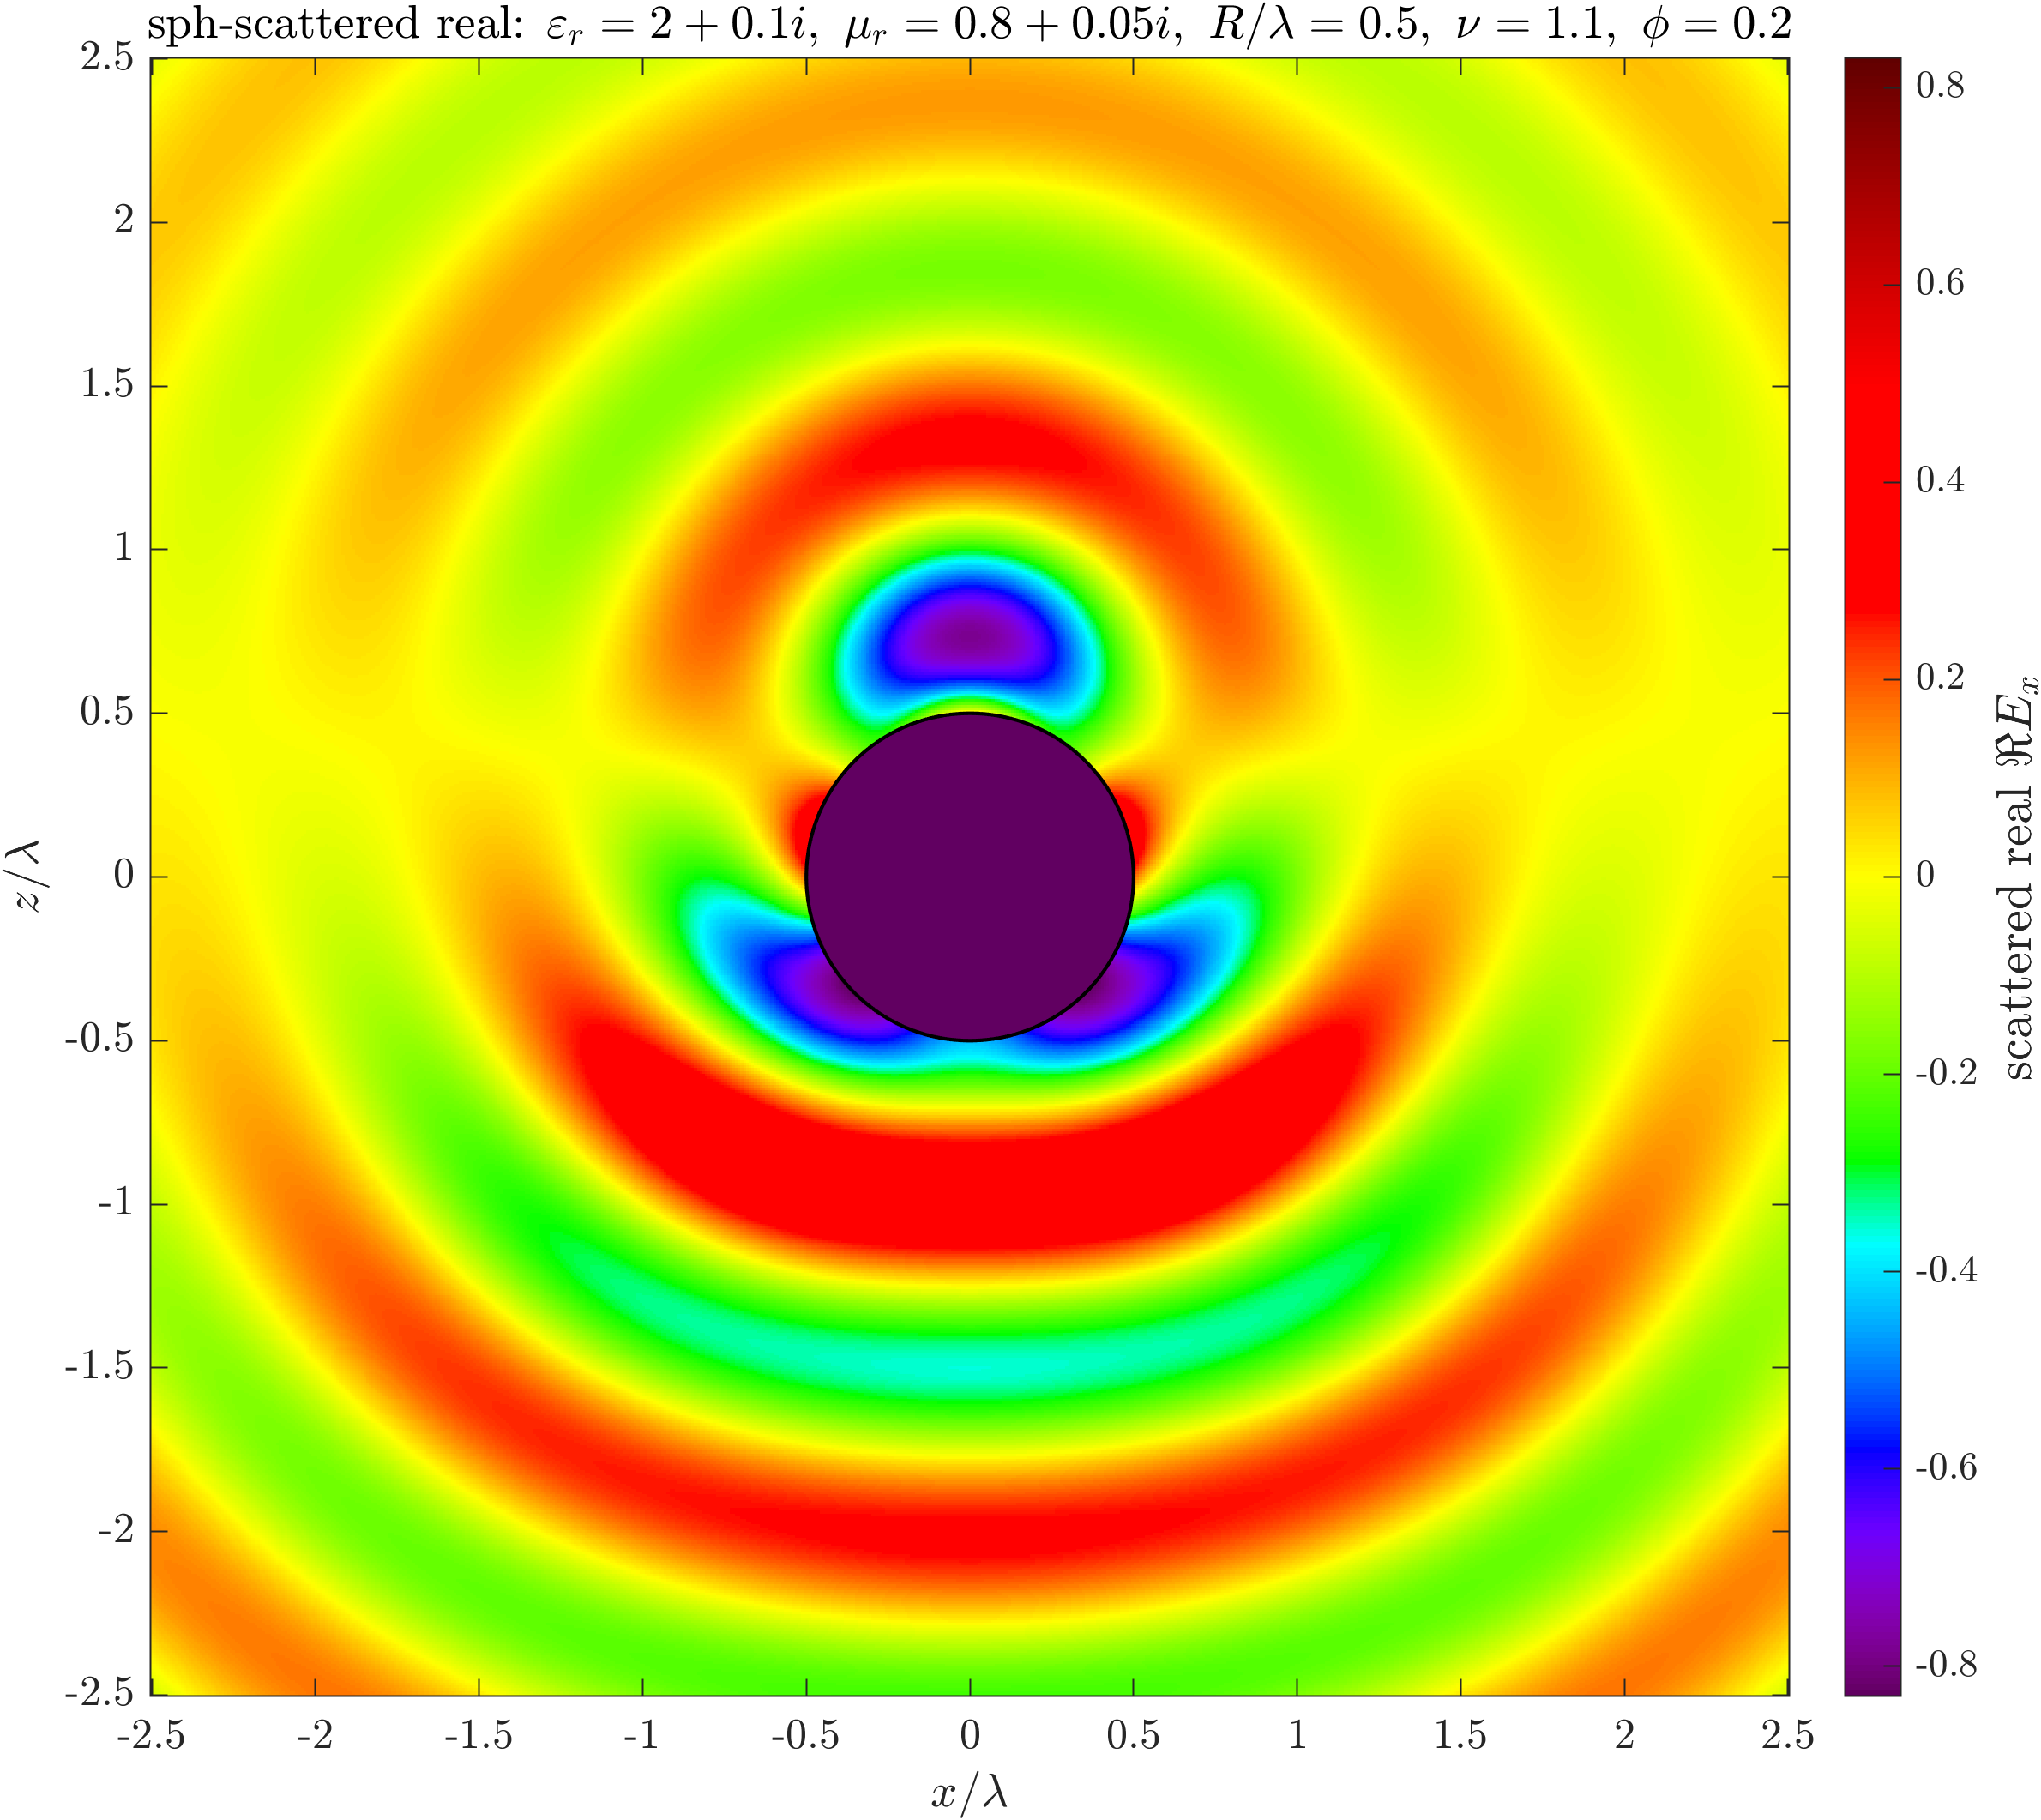
\includegraphics[width=\linewidth]{scattering_fig/lossy_small_sphere_x_direction_real_part.png}
			\caption{有损小球，\(x\)方向实部}
			\label{球体散射振幅比较图(对比有无损耗及不同半径)-有损小球,x方向实部}
		\end{subfigure}
		\hfill
		\begin{subfigure}{0.235\textwidth}
			\centering
			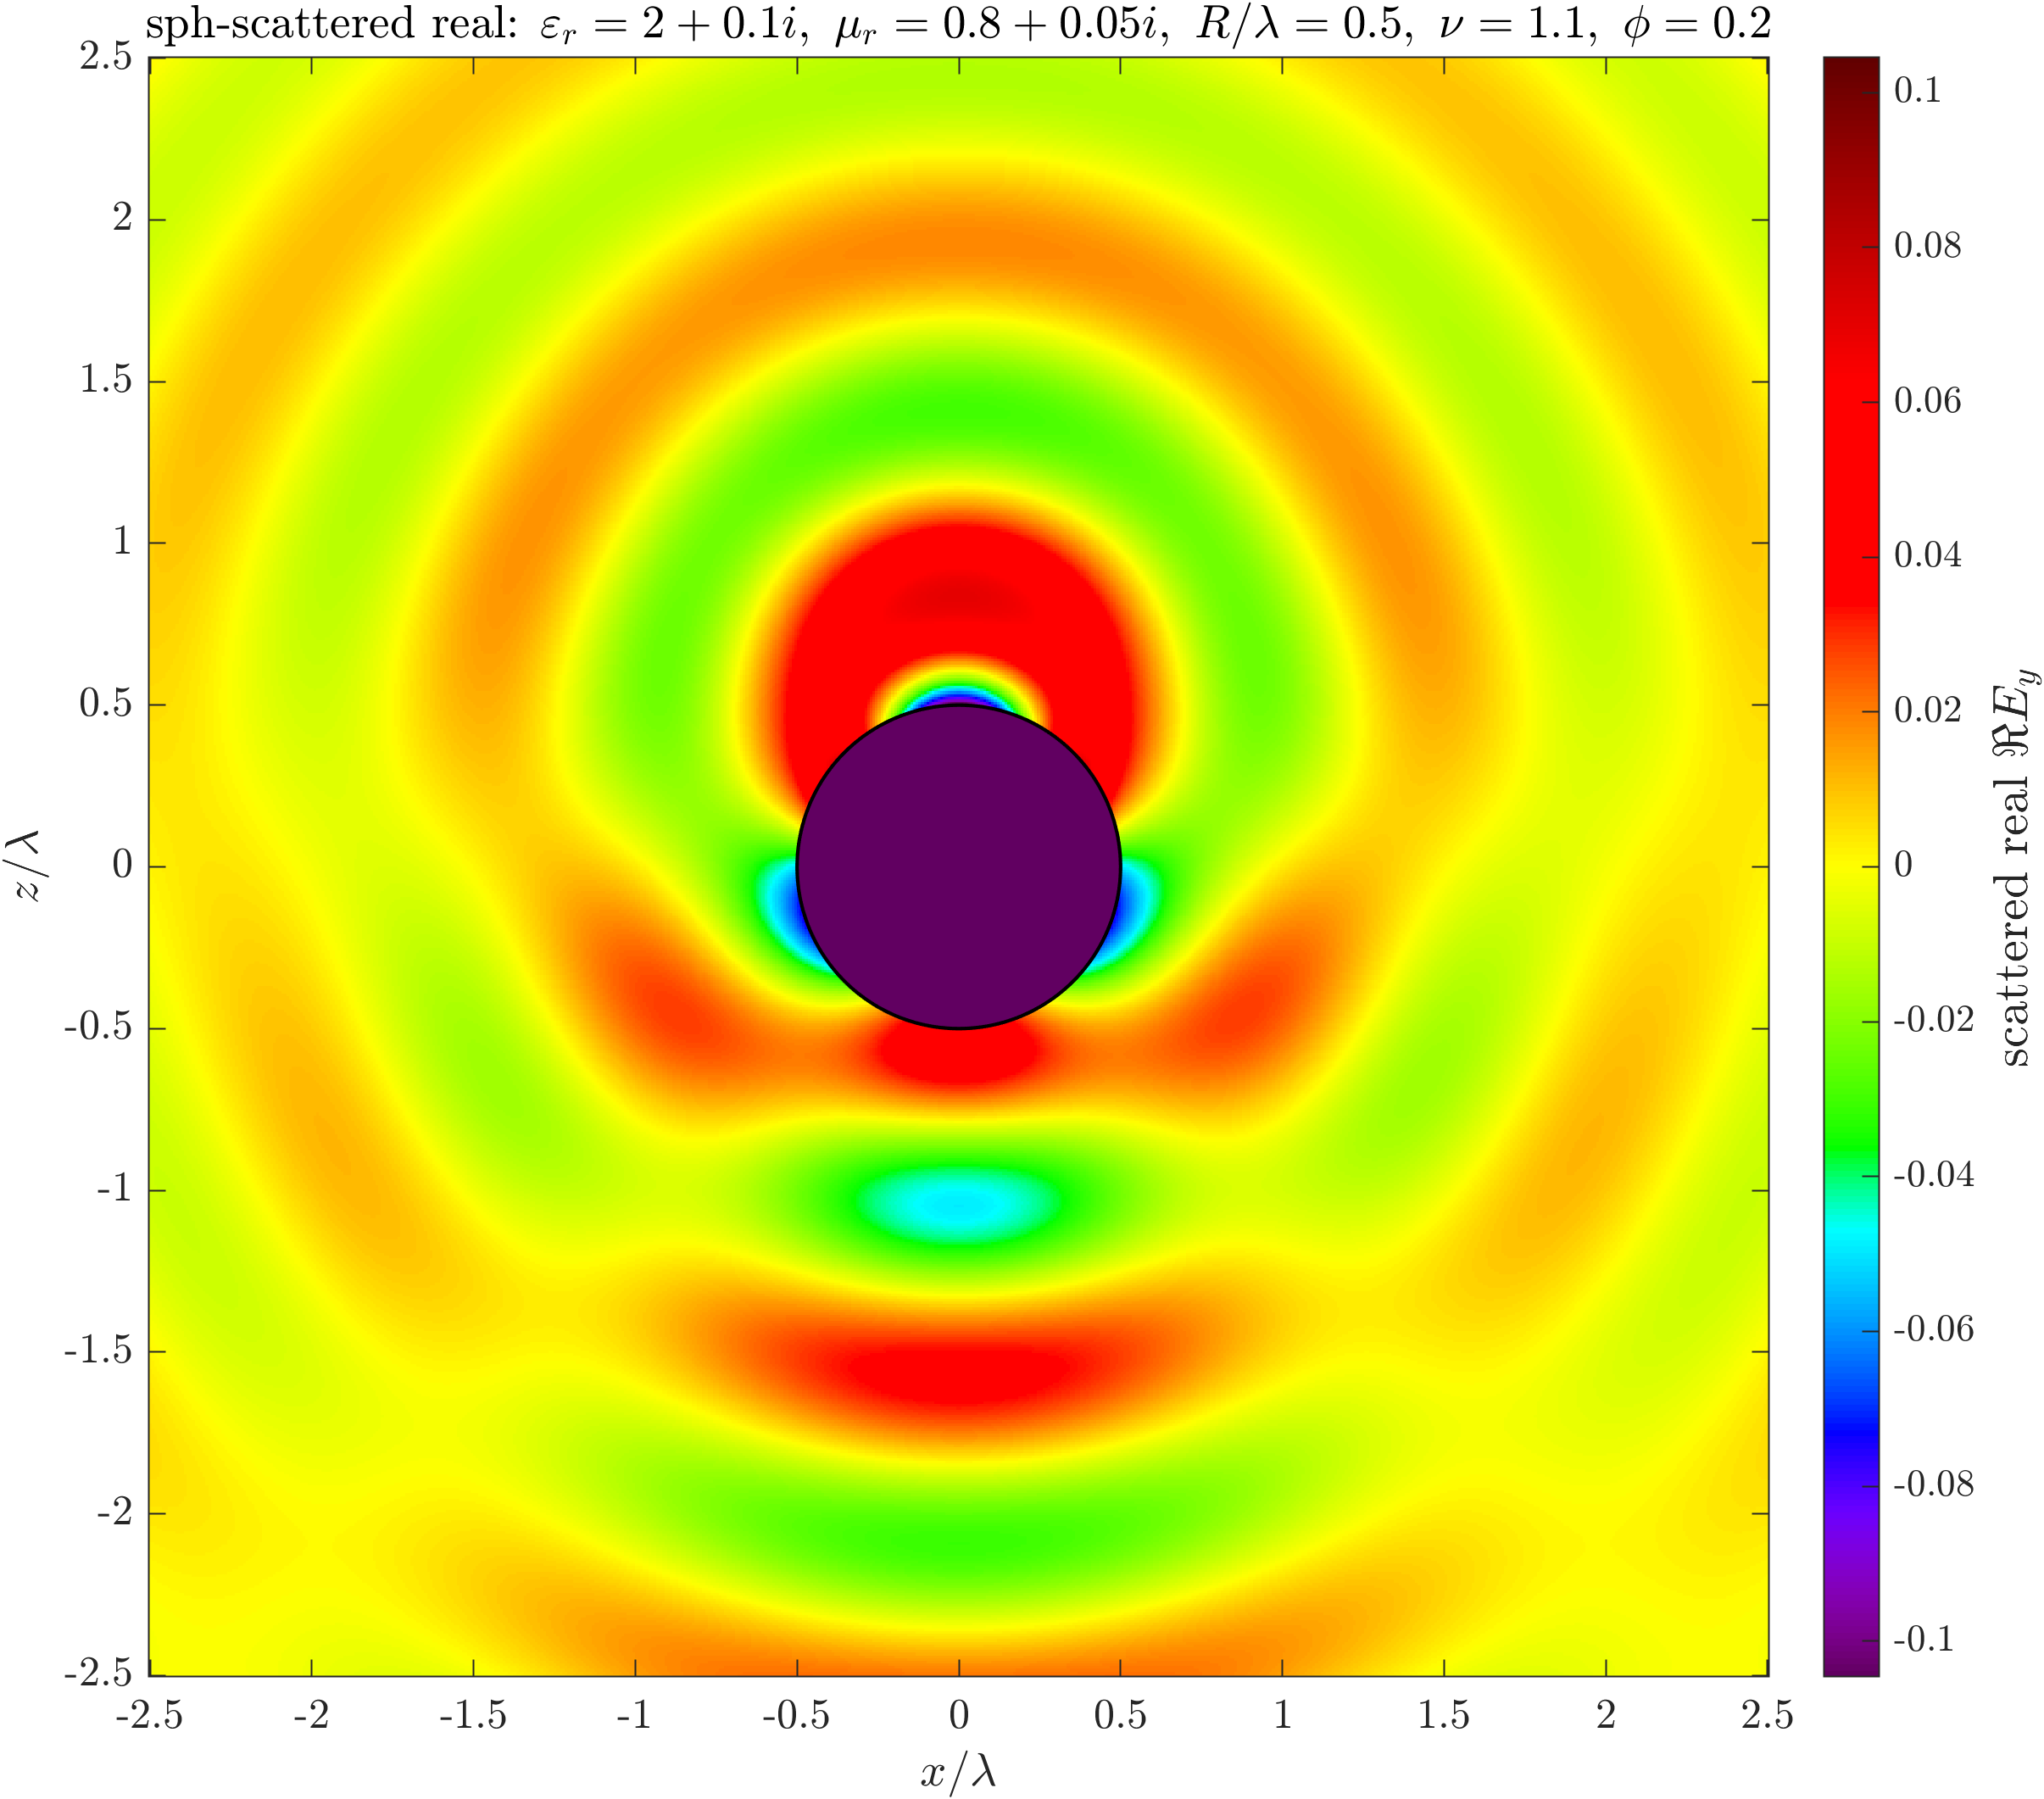
\includegraphics[width=\linewidth]{scattering_fig/lossy_small_sphere_y_direction_real_part.png}
			\caption{有损小球，\(y\)方向实部}
			\label{球体散射振幅比较图(对比有无损耗及不同半径)-有损小球,y方向实部}
		\end{subfigure}
		\hfill
		\begin{subfigure}{0.235\textwidth}
			\centering
			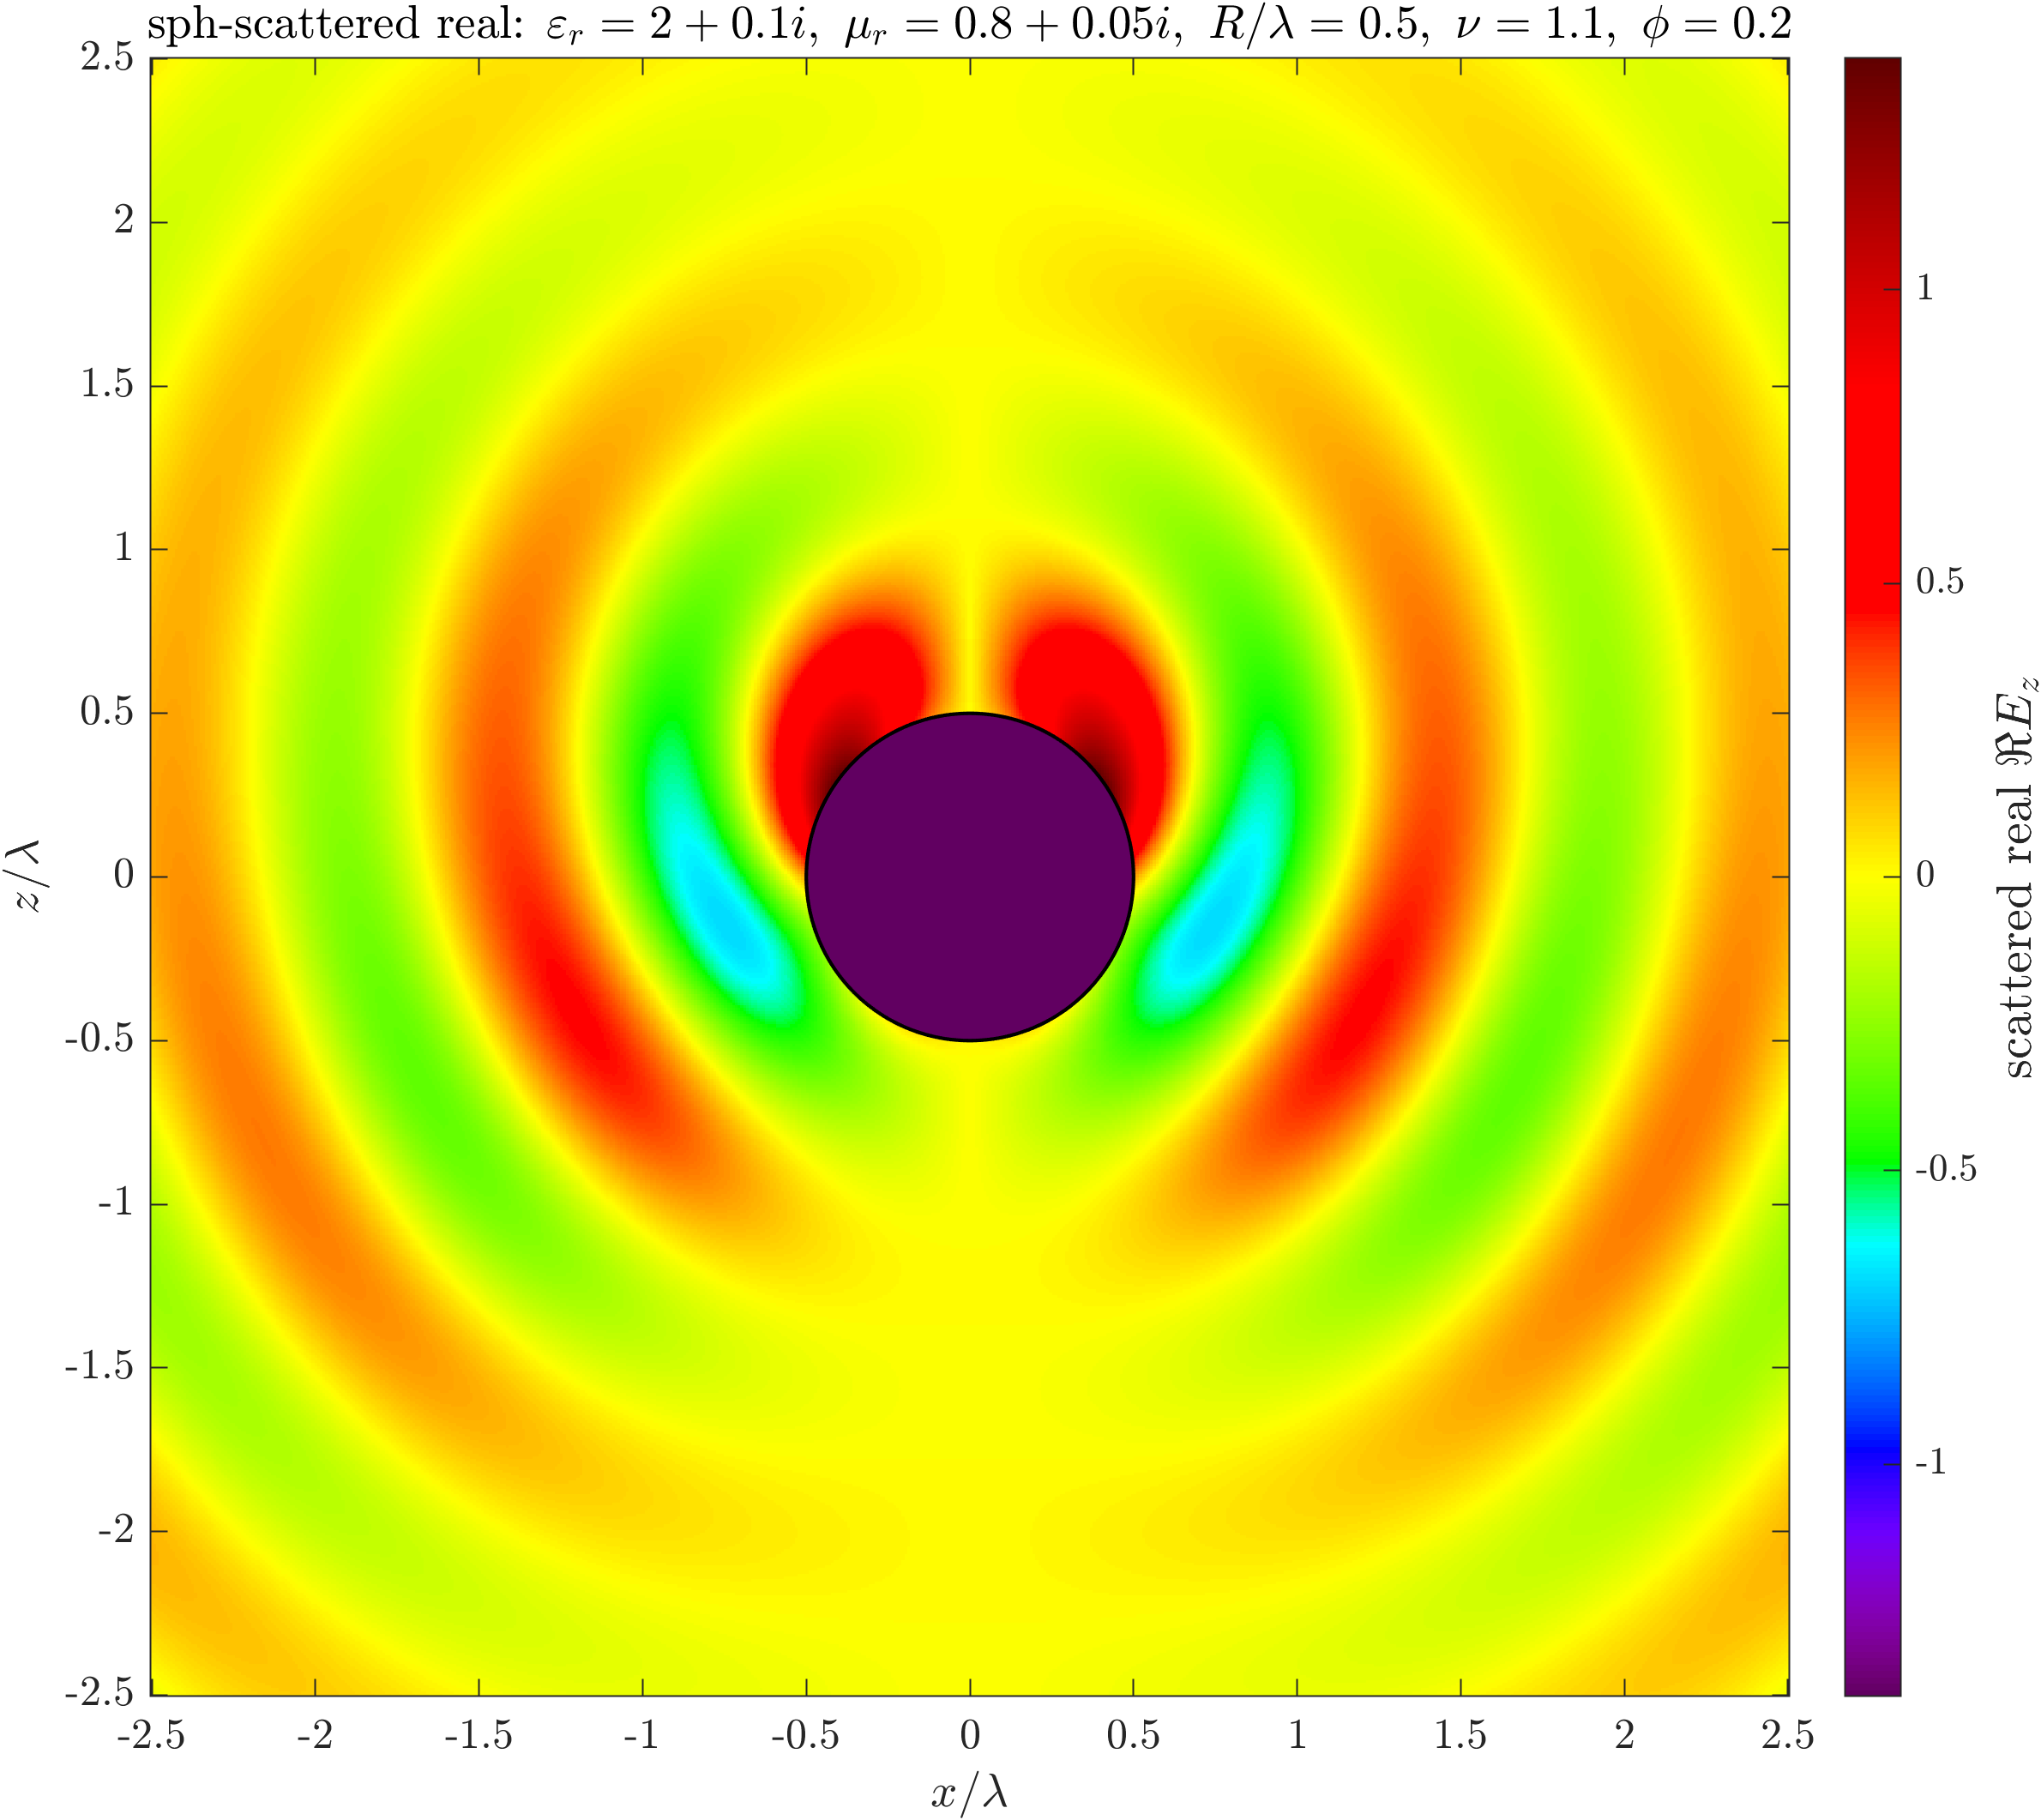
\includegraphics[width=\linewidth]{scattering_fig/lossy_small_sphere_z_direction_real_part.png}
			\caption{有损小球，\(z\)方向实部}
			\label{球体散射振幅比较图(对比有无损耗及不同半径)-有损小球,z方向实部}
		\end{subfigure}
		\hfill
		\begin{subfigure}{0.235\textwidth}
			\centering
			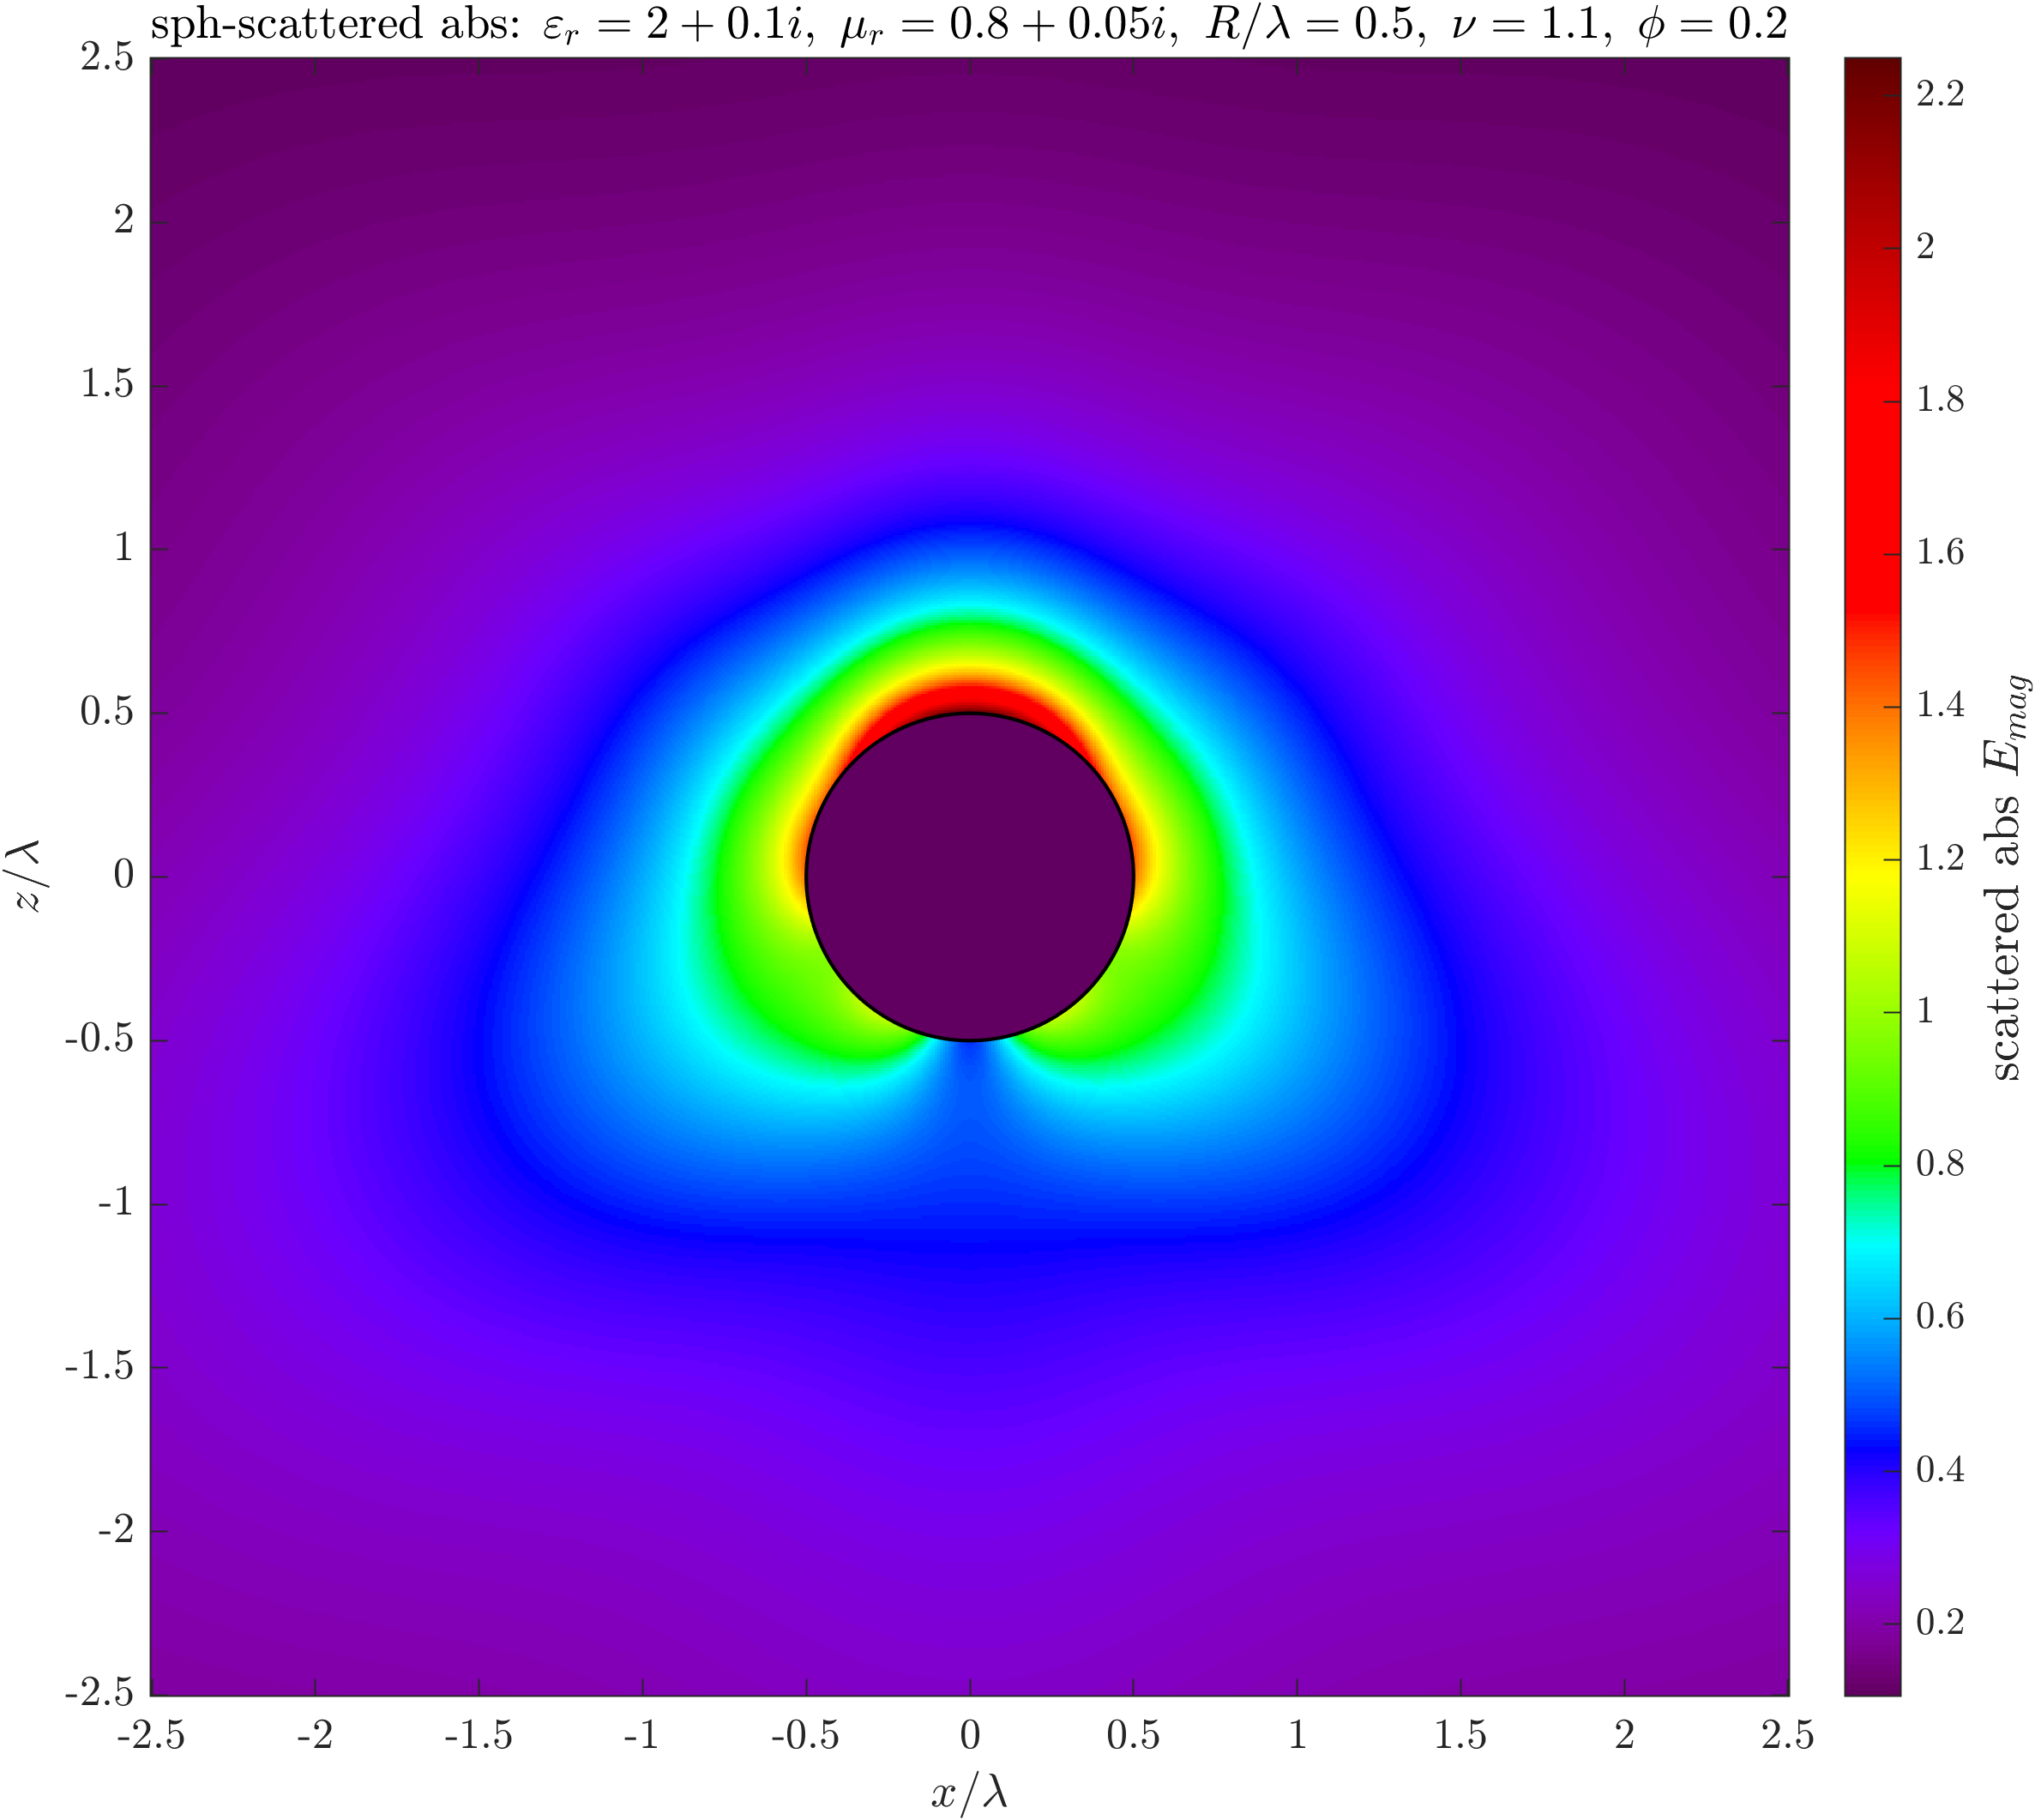
\includegraphics[width=\linewidth]{scattering_fig/lossy_small_sphere_amplitude_magnitude.png}
			\caption{有损小球，振幅大小}
			\label{球体散射振幅比较图(对比有无损耗及不同半径)-有损小球,振幅大小}
		\end{subfigure}

		\vspace{1em}

		% 第二行：有损大球 (R/lambda=1.2, 有损耗)
		\begin{subfigure}{0.235\textwidth}
			\centering
			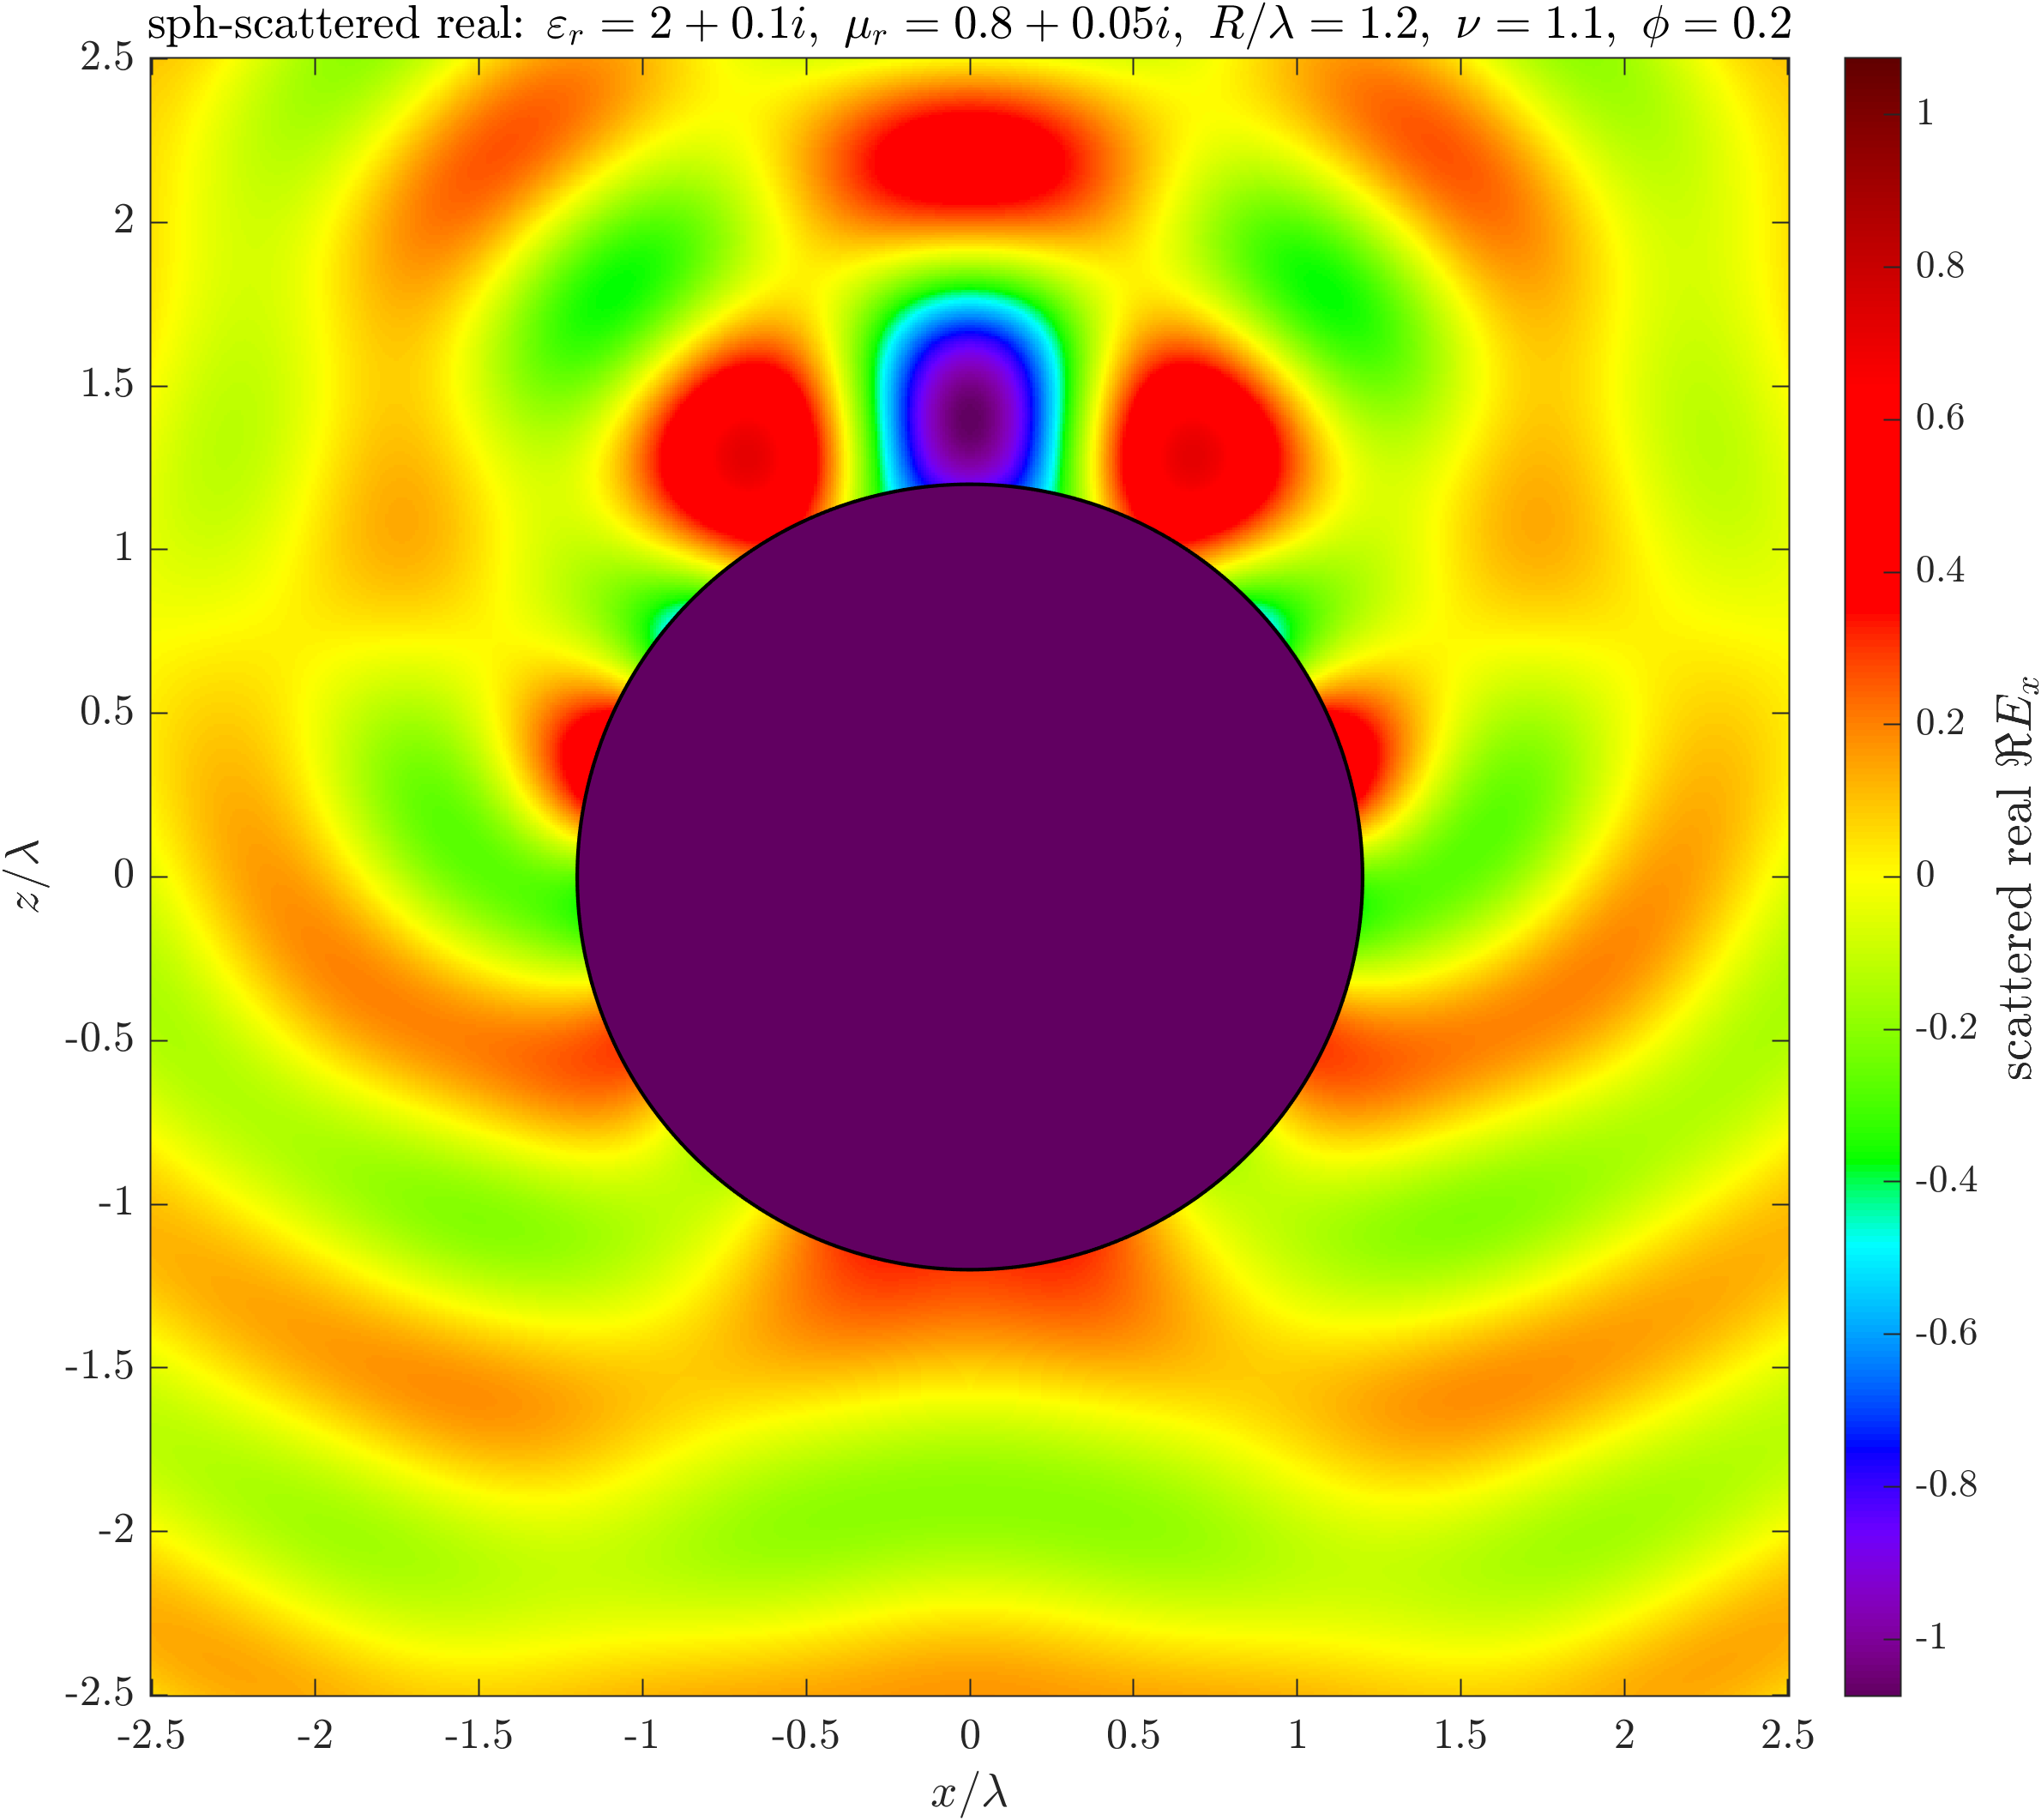
\includegraphics[width=\linewidth]{scattering_fig/lossy_large_sphere_x_direction_real_part.png}
			\caption{有损大球，\(x\)方向实部}
			\label{球体散射振幅比较图(对比有无损耗及不同半径)-有损大球,x方向实部}
		\end{subfigure}
		\hfill
		\begin{subfigure}{0.235\textwidth}
			\centering
			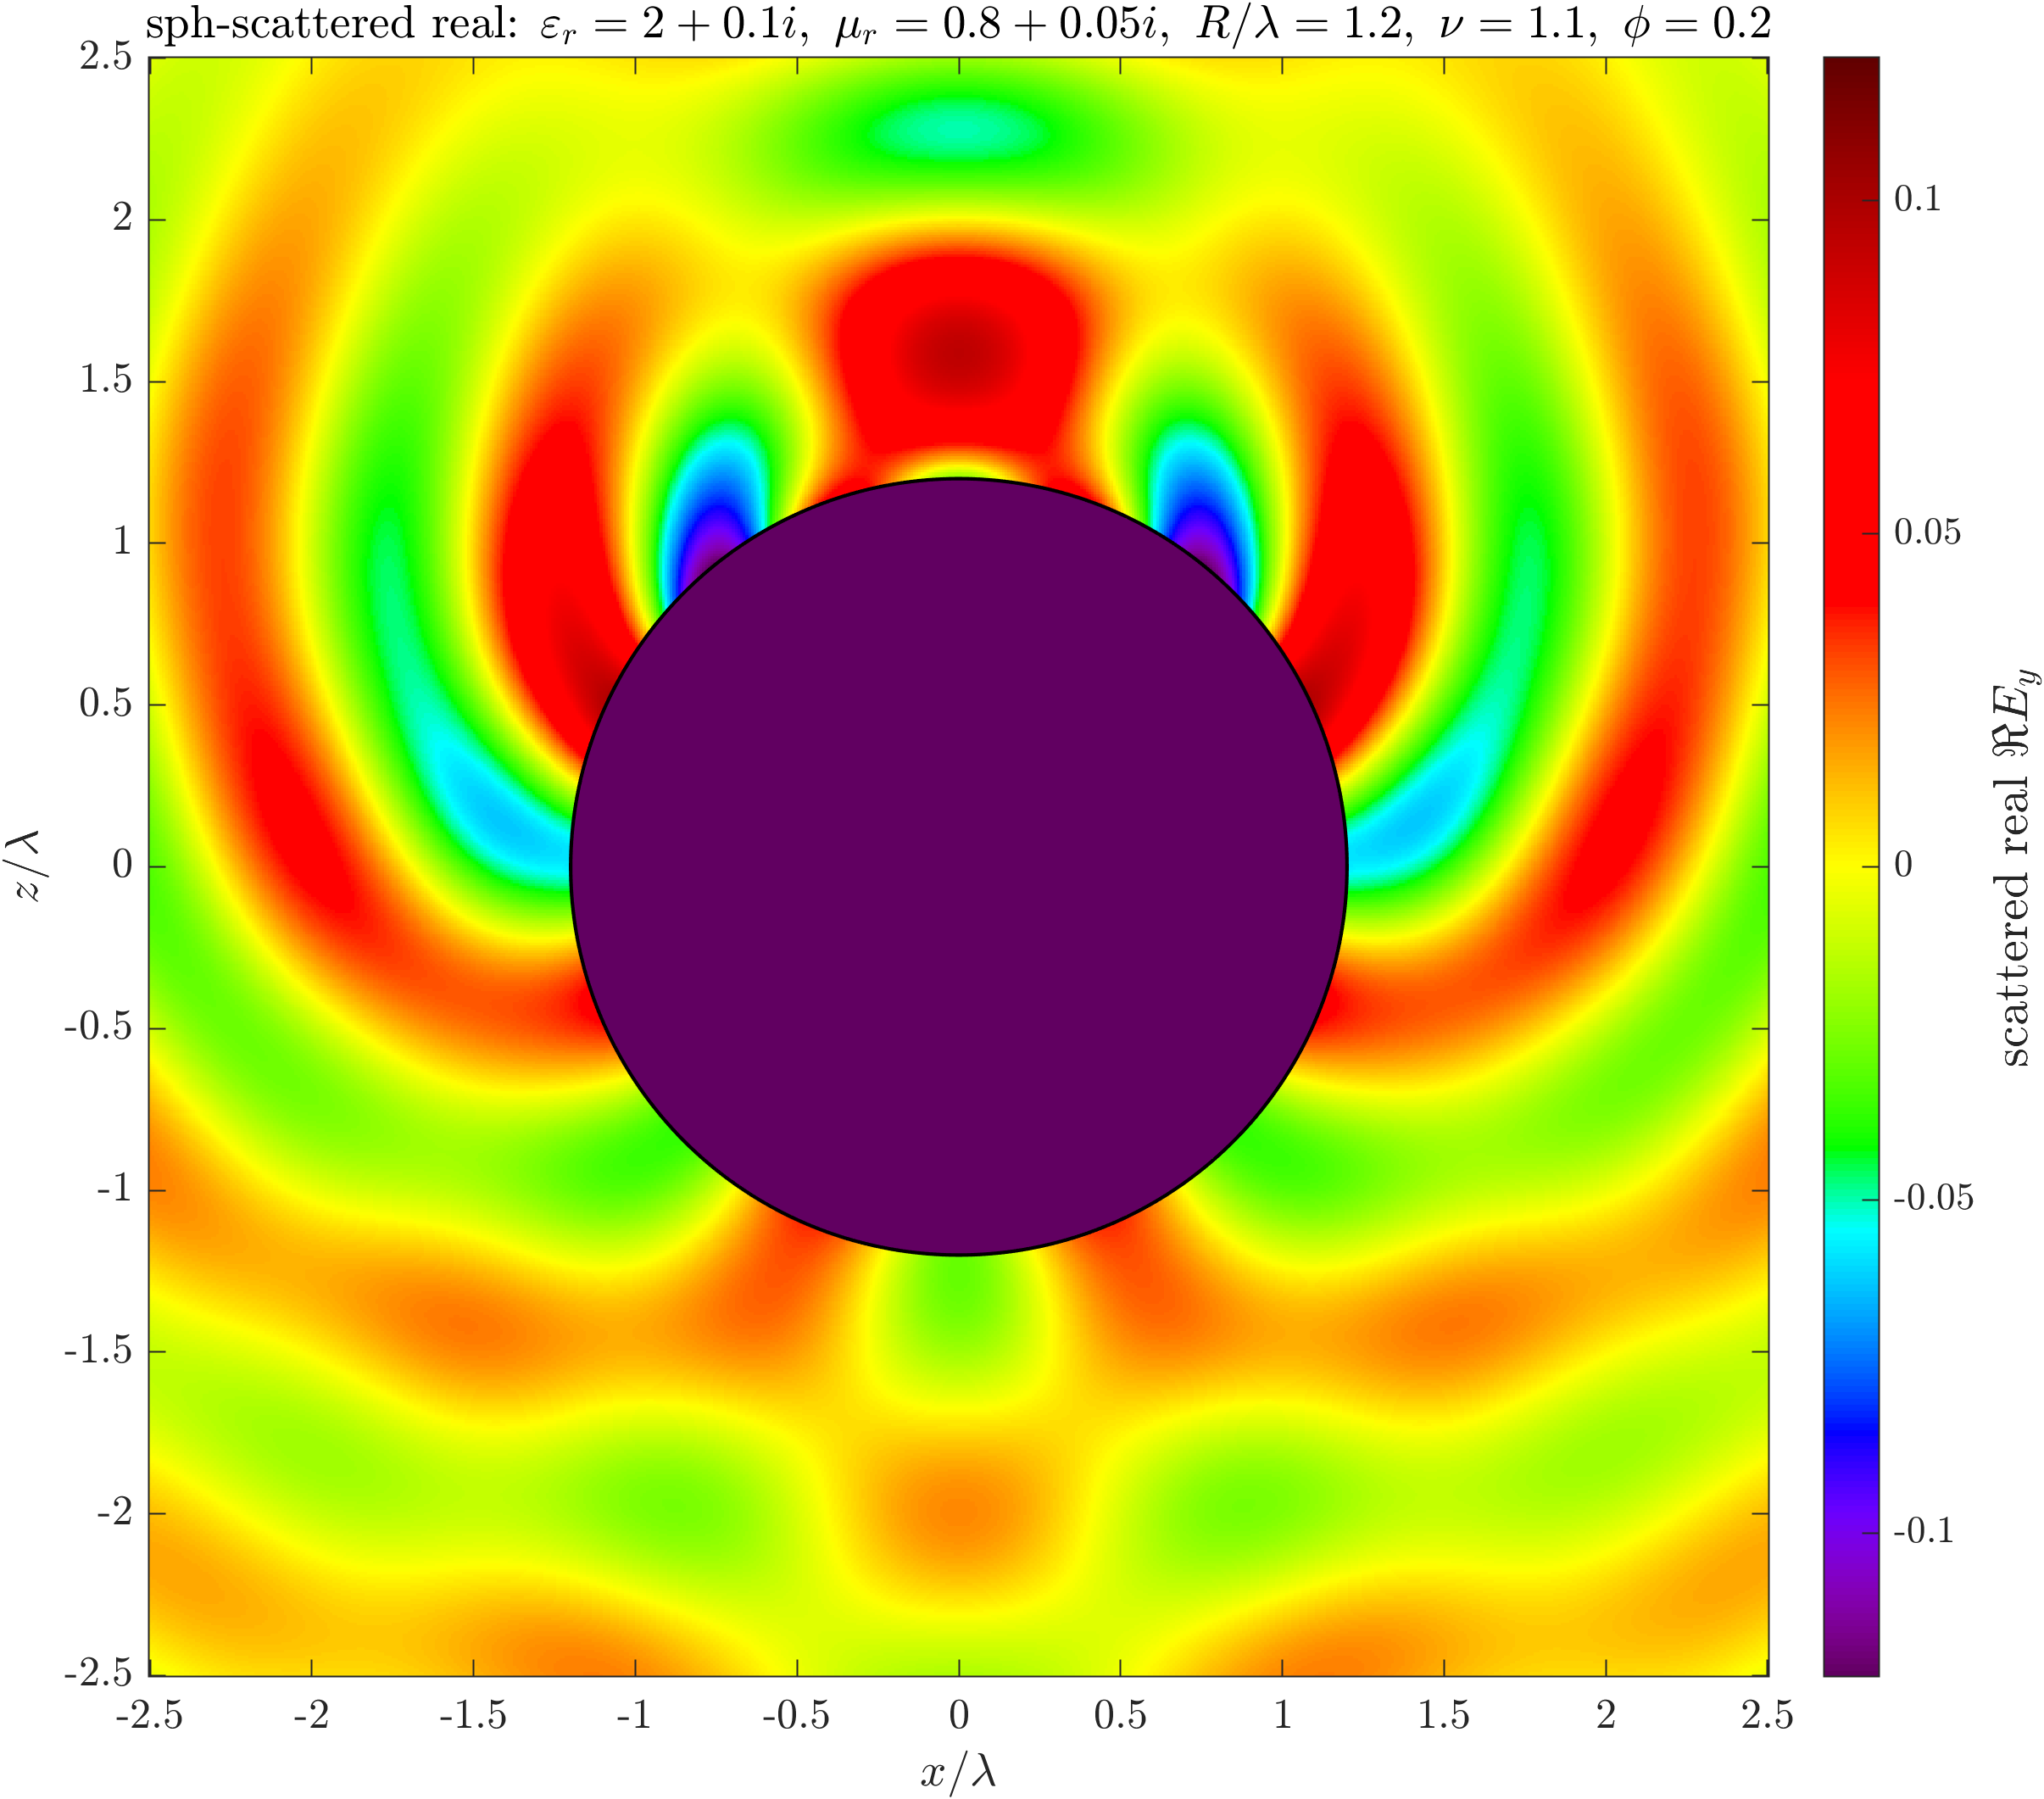
\includegraphics[width=\linewidth]{scattering_fig/lossy_large_sphere_y_direction_real_part.png}
			\caption{有损大球，\(y\)方向实部}
			\label{球体散射振幅比较图(对比有无损耗及不同半径)-有损大球,y方向实部}
		\end{subfigure}
		\hfill
		\begin{subfigure}{0.235\textwidth}
			\centering
			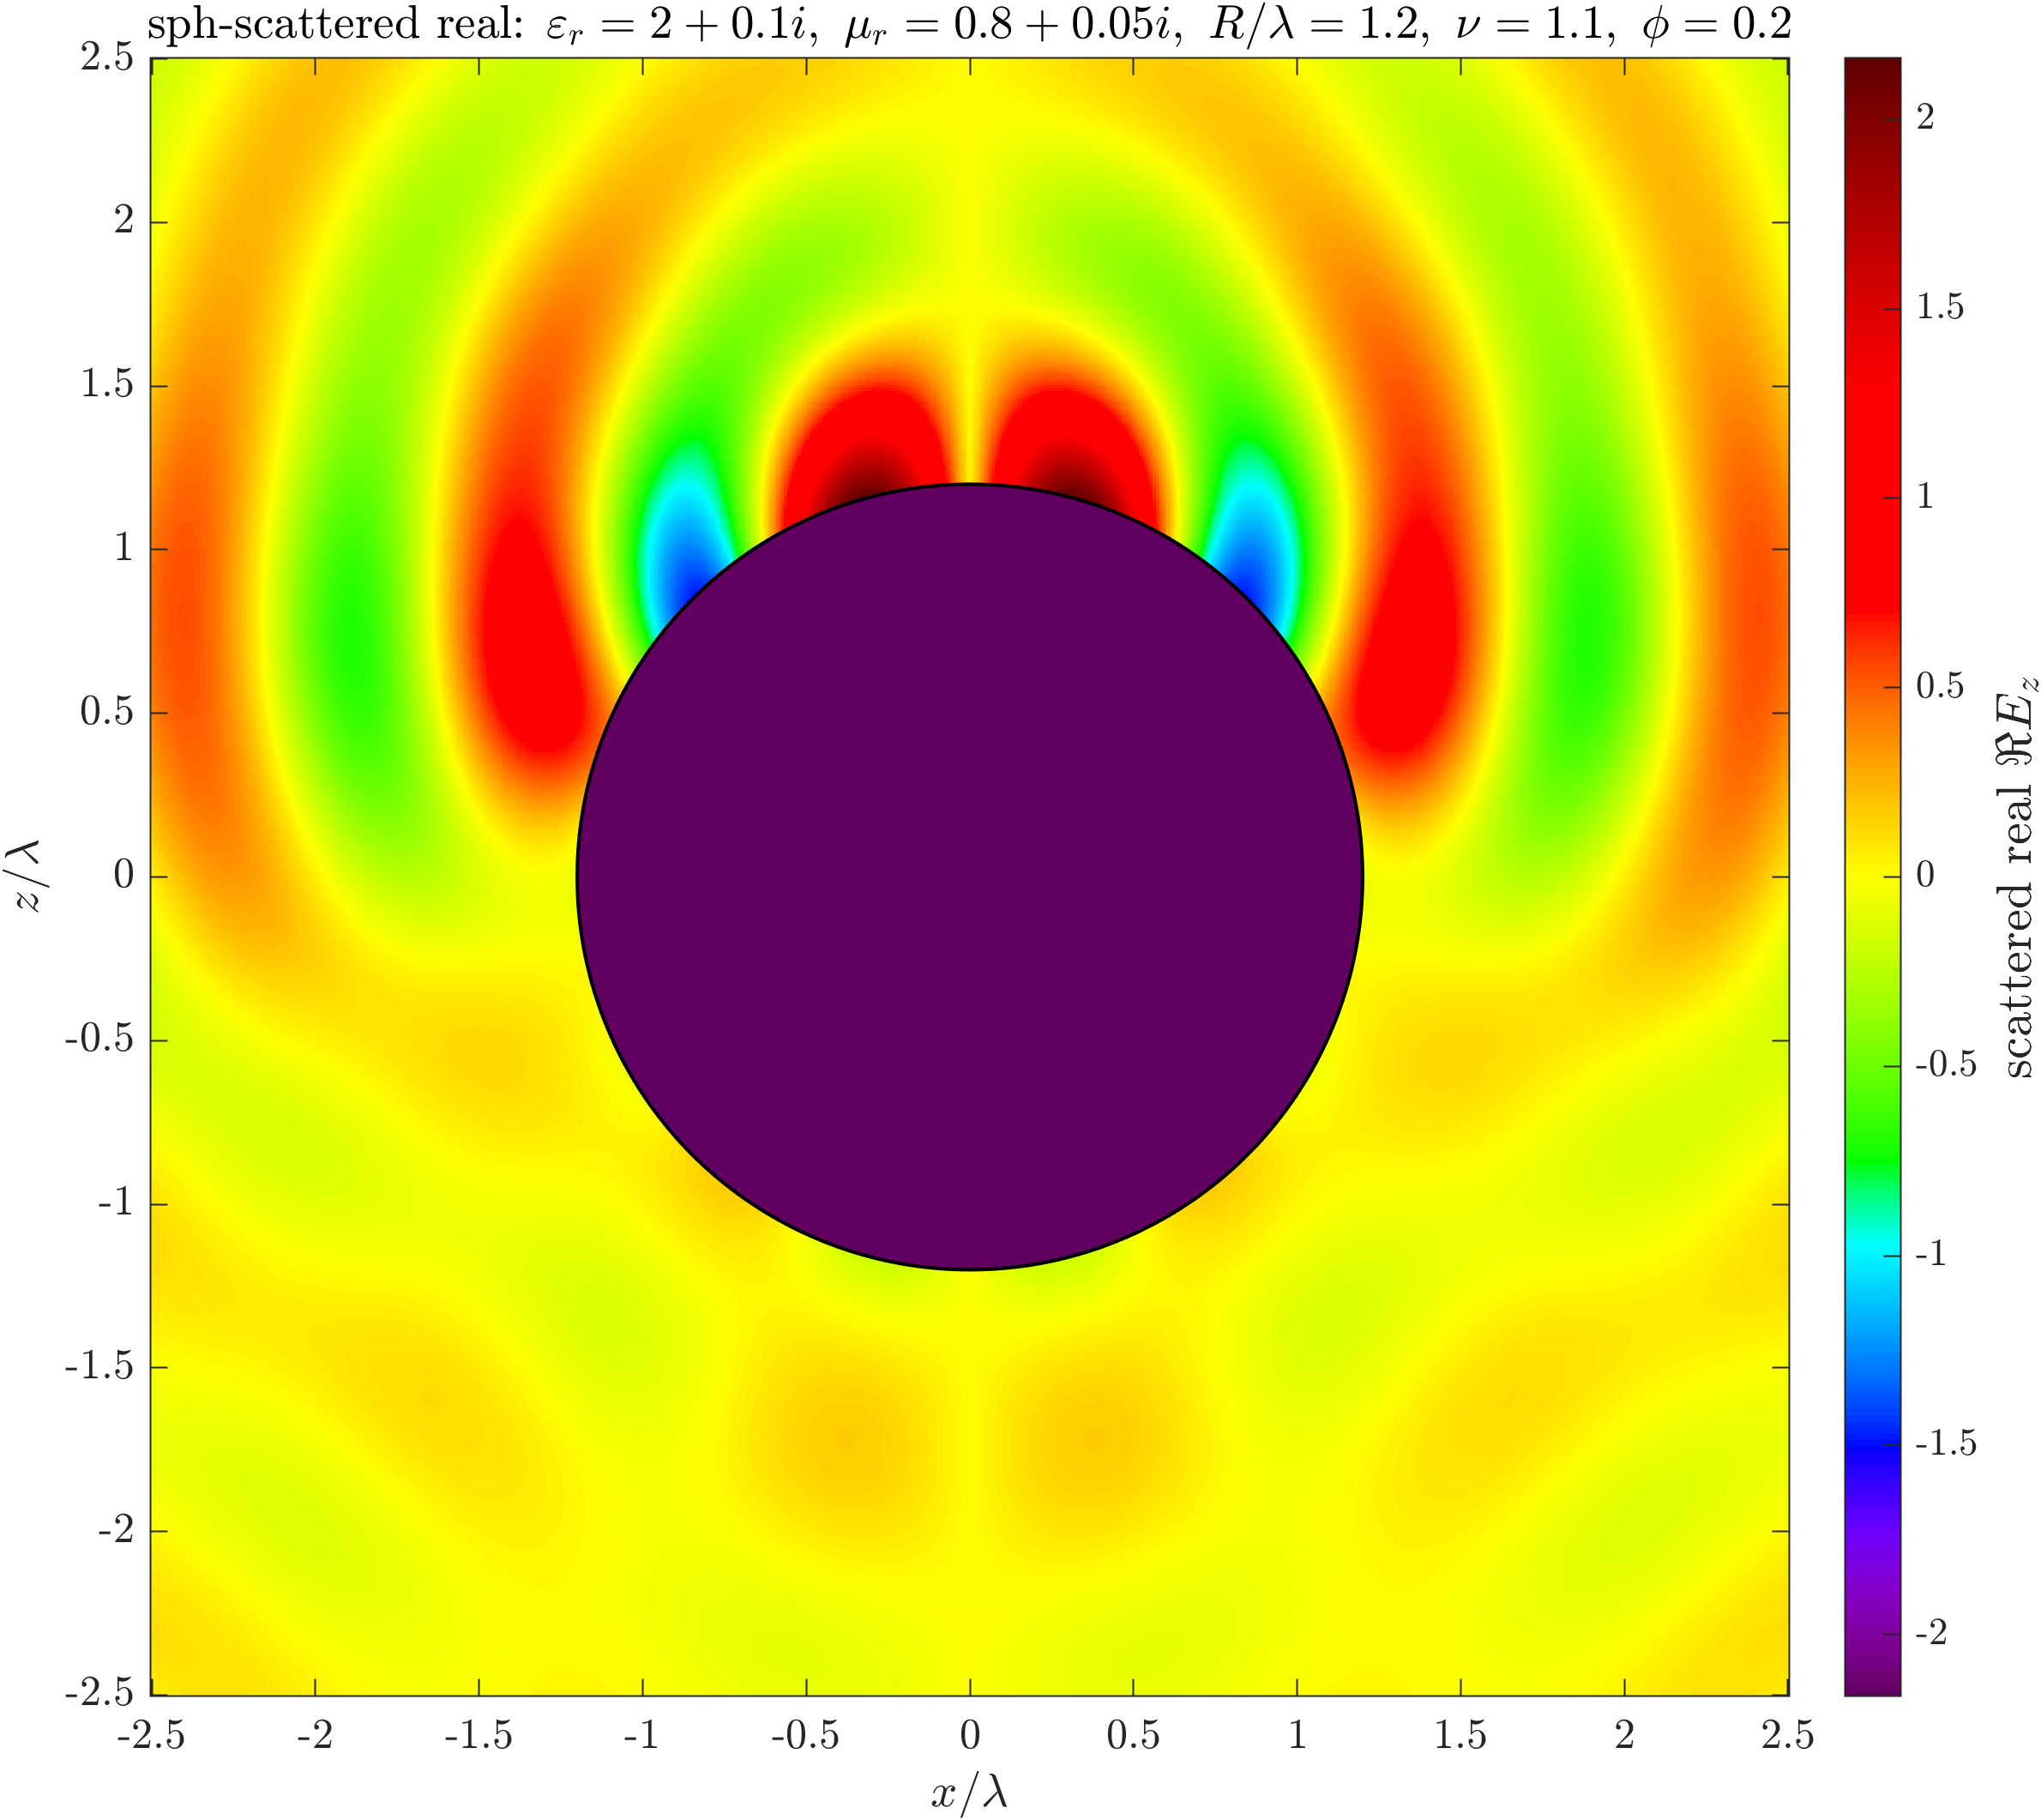
\includegraphics[width=\linewidth]{scattering_fig/lossy_large_sphere_z_direction_real_part.png}
			\caption{有损大球，\(z\)方向实部}
			\label{球体散射振幅比较图(对比有无损耗及不同半径)-有损大球,z方向实部}
		\end{subfigure}
		\hfill
		\begin{subfigure}{0.235\textwidth}
			\centering
			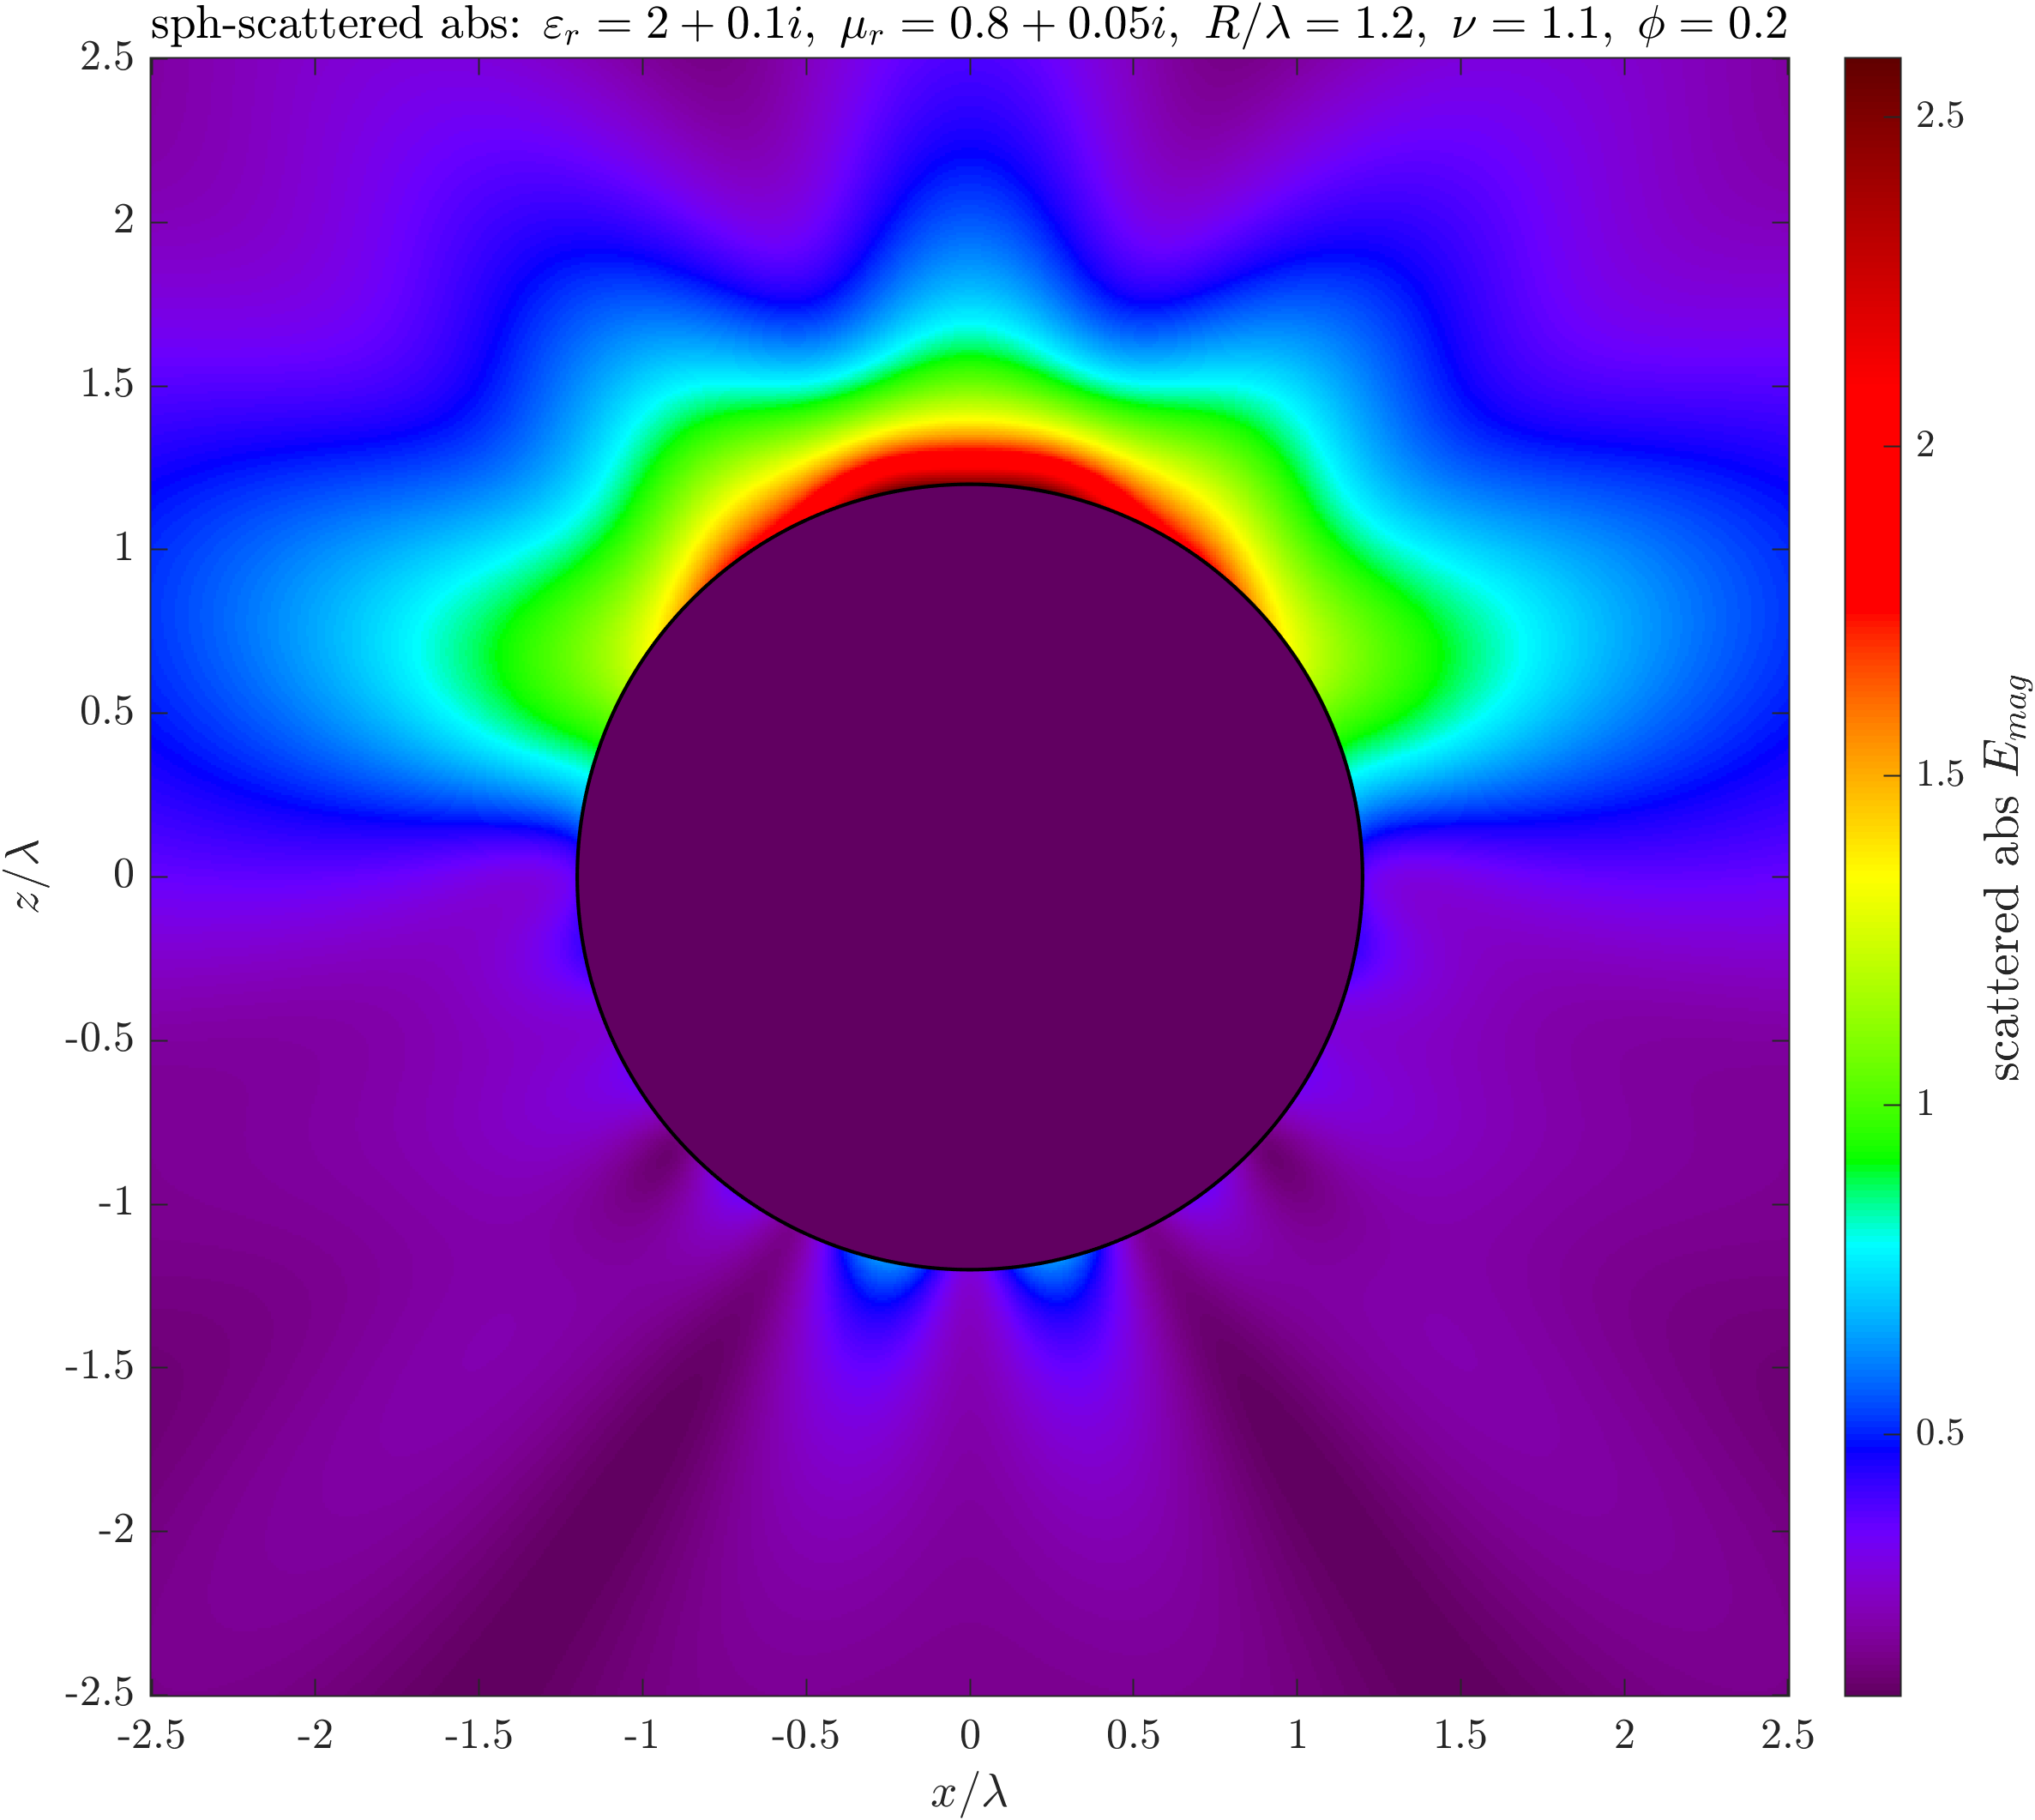
\includegraphics[width=\linewidth]{scattering_fig/lossy_large_sphere_amplitude_magnitude.png}
			\caption{有损大球，振幅大小}
			\label{球体散射振幅比较图(对比有无损耗及不同半径)-有损大球,振幅大小}
		\end{subfigure}

		\vspace{1em}

		% 第三行：无损大球 (R/lambda=1.2, 无损耗)
		\begin{subfigure}{0.235\textwidth}
			\centering
			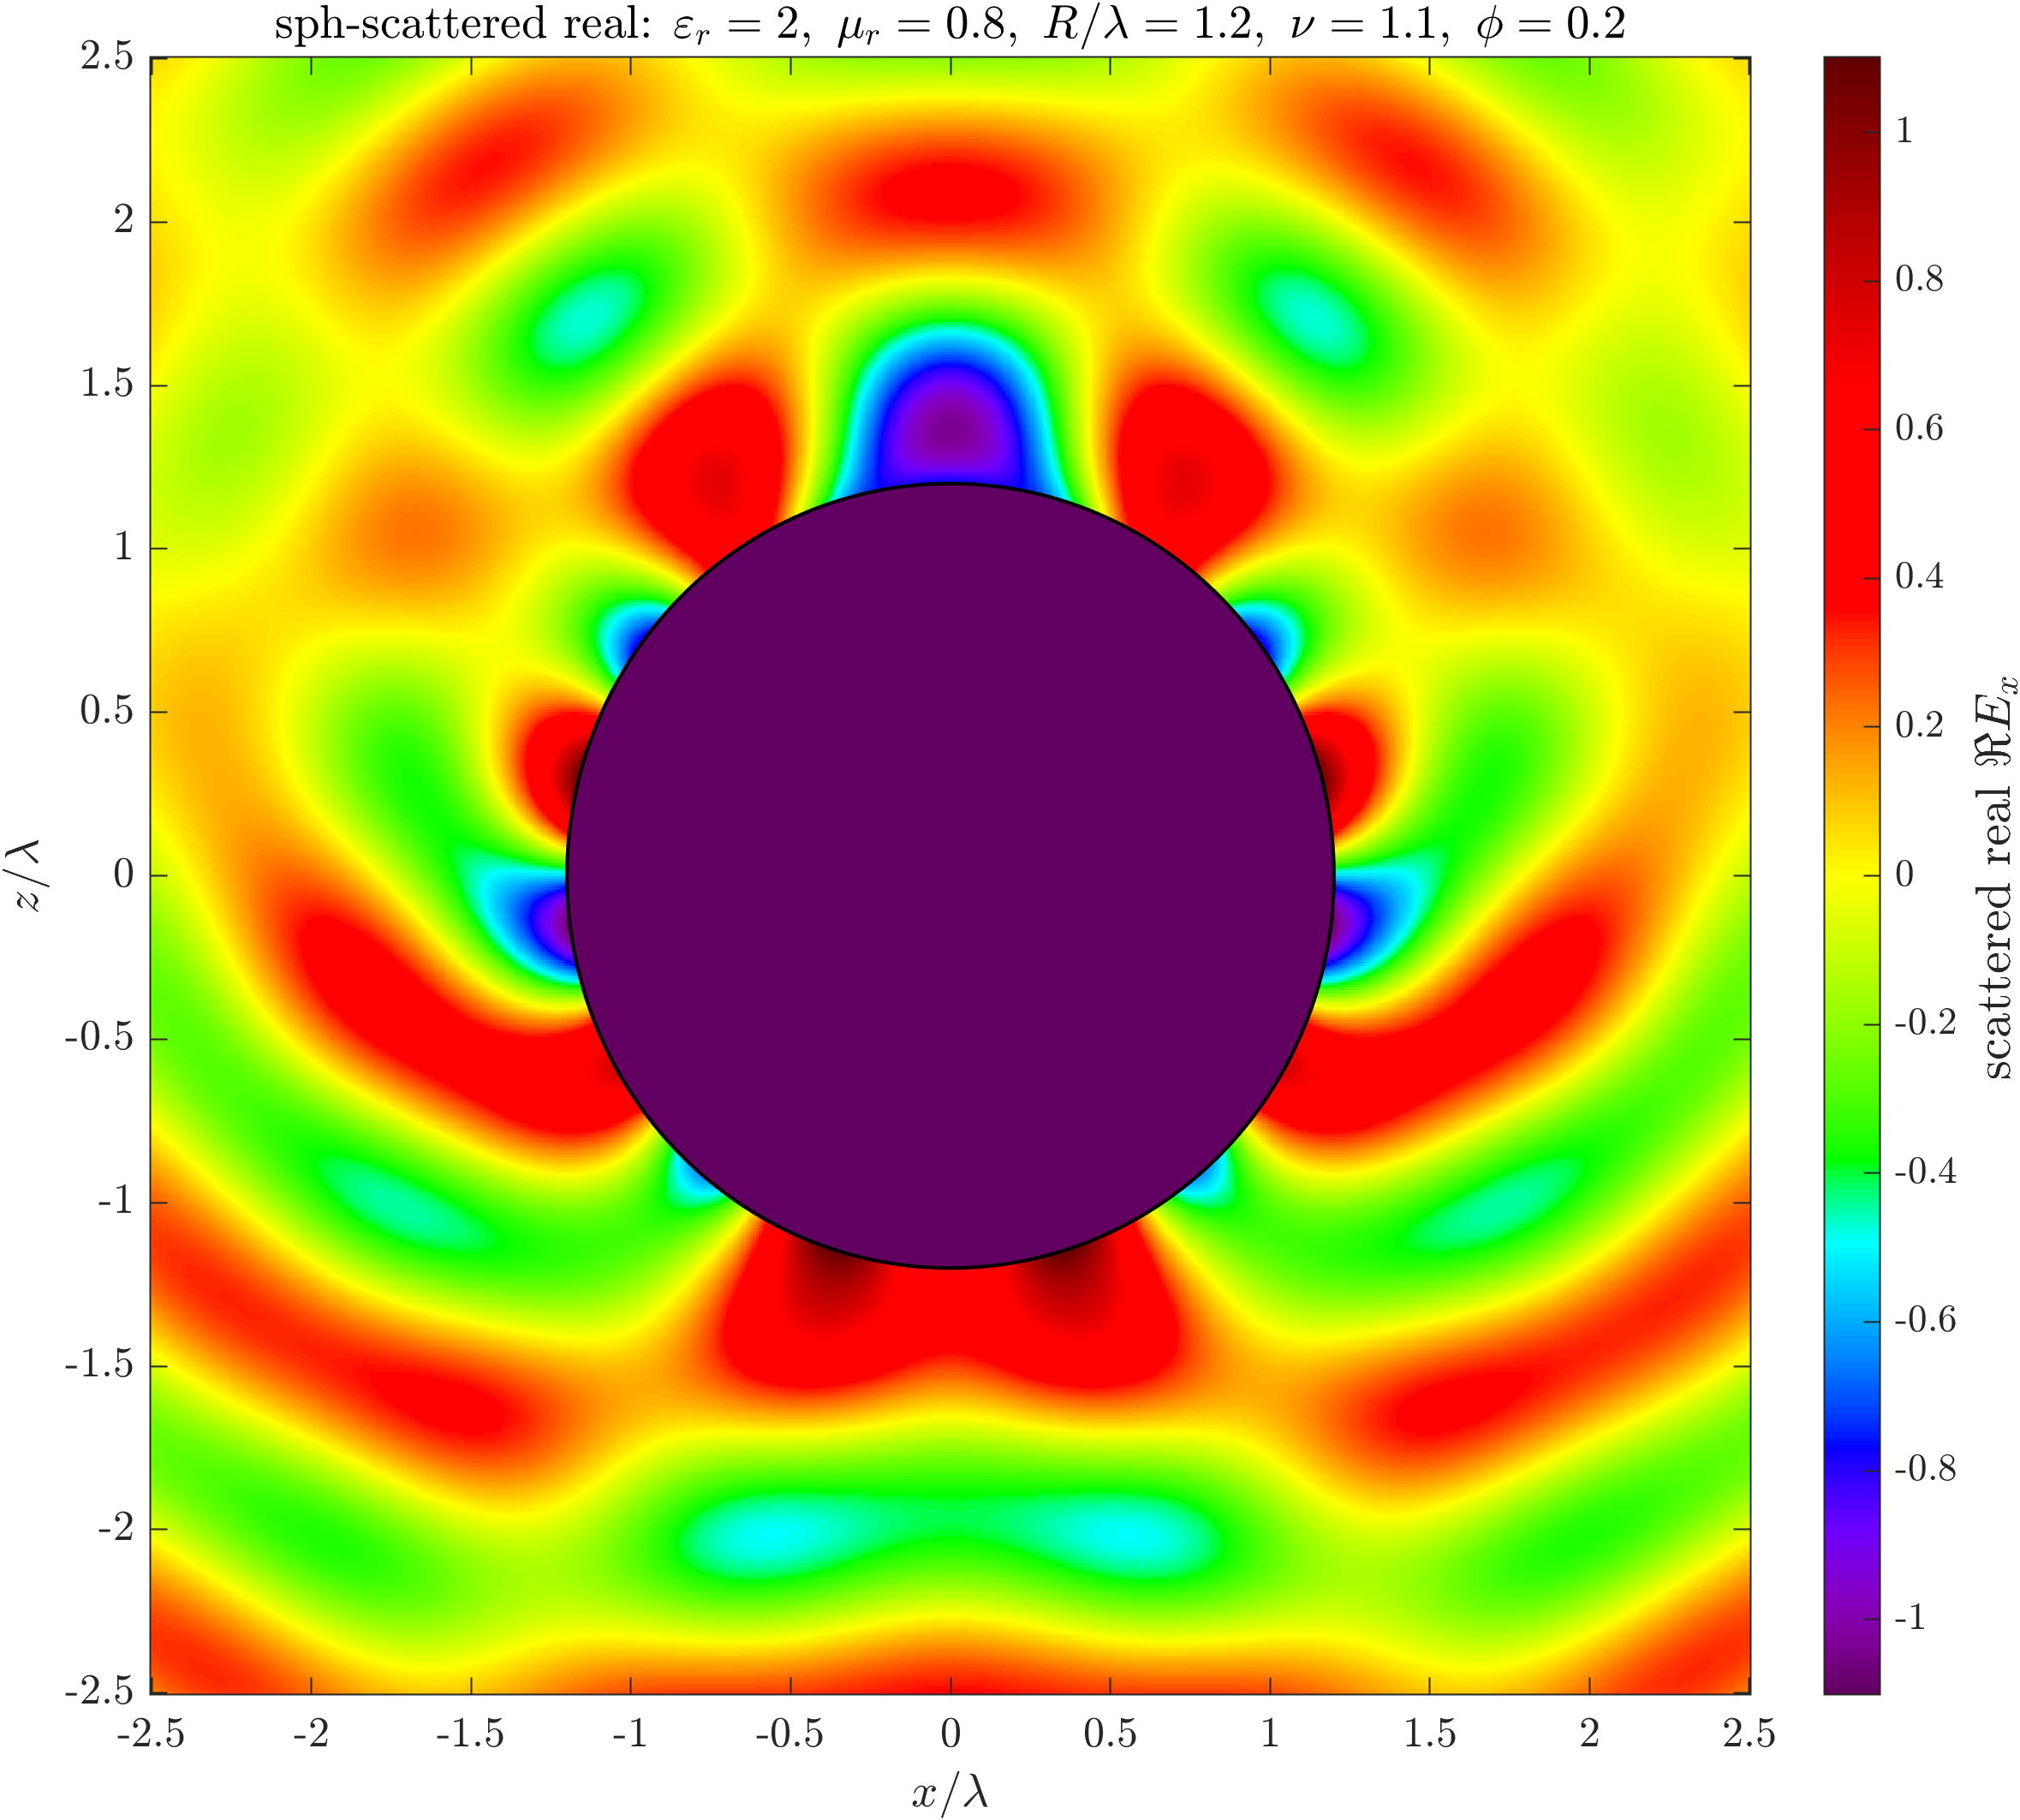
\includegraphics[width=\linewidth]{scattering_fig/lossless_large_sphere_x_direction_real_part.png}
			\caption{无损大球，\(x\)方向实部}
			\label{球体散射振幅比较图(对比有无损耗及不同半径)-无损大球,x方向实部}
		\end{subfigure}
		\hfill
		\begin{subfigure}{0.235\textwidth}
			\centering
			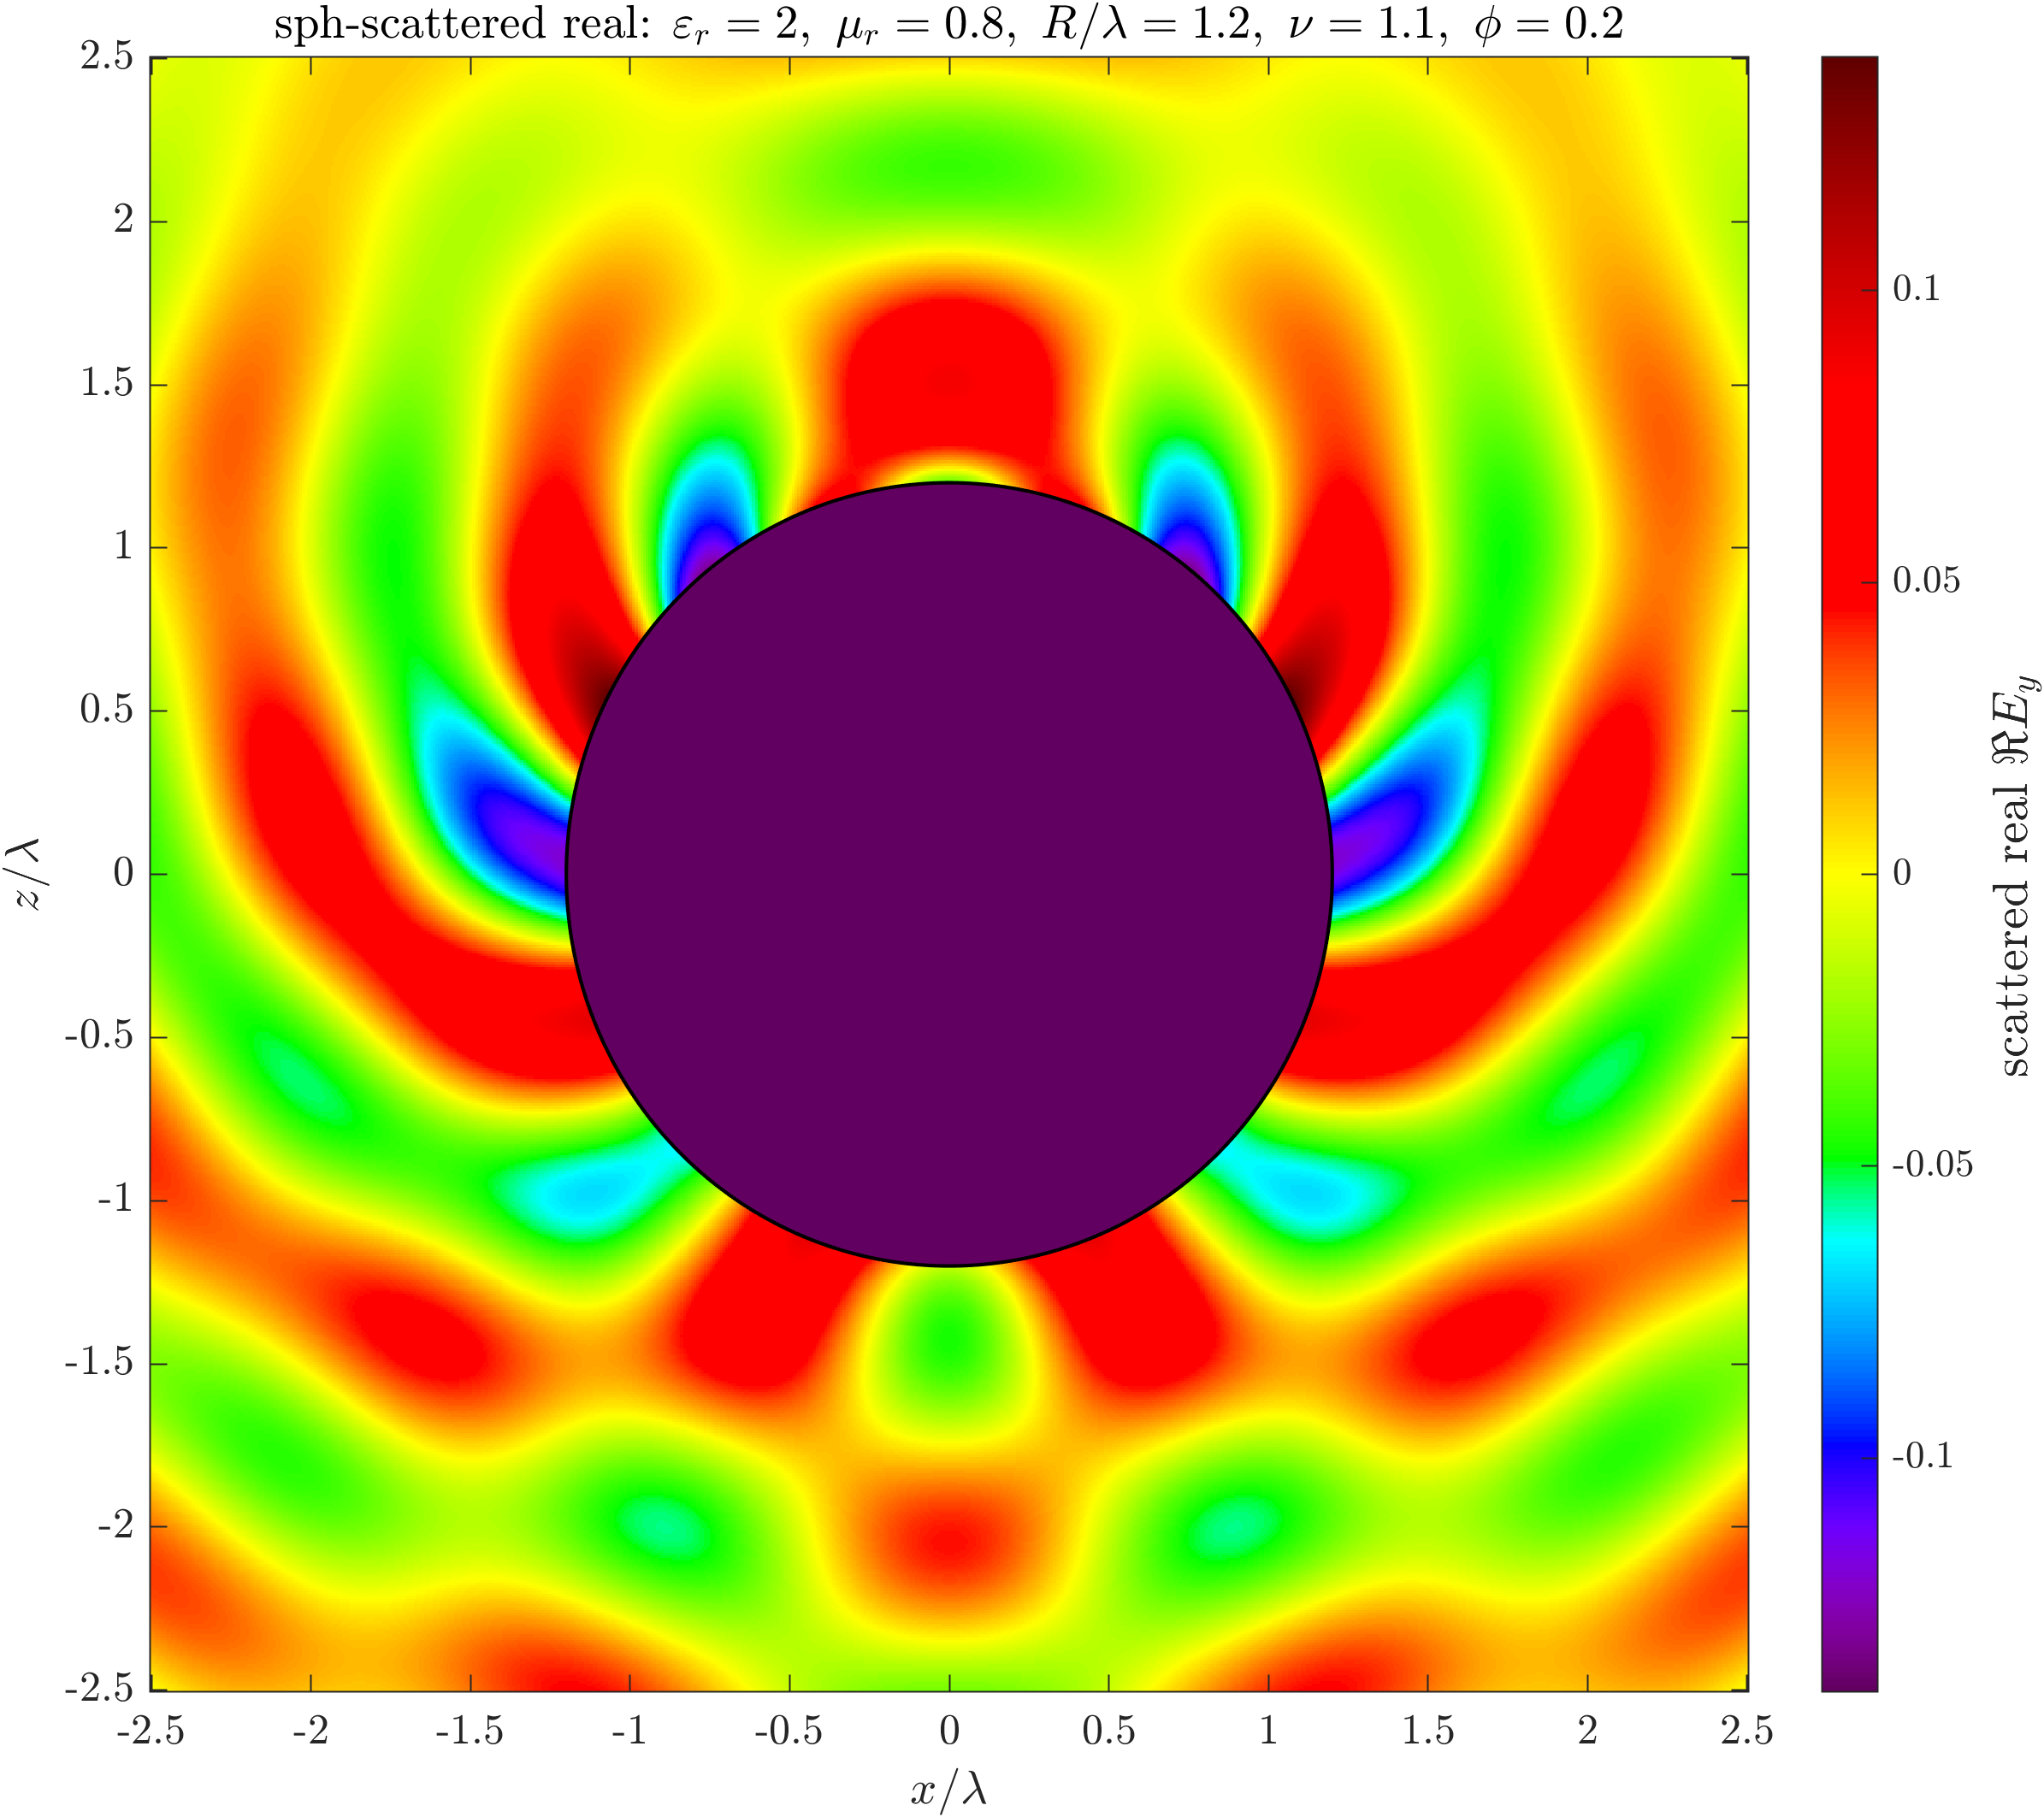
\includegraphics[width=\linewidth]{scattering_fig/lossless_large_sphere_y_direction_real_part.png}
			\caption{无损大球，\(y\)方向实部}
			\label{球体散射振幅比较图(对比有无损耗及不同半径)-无损大球,y方向实部}
		\end{subfigure}
		\hfill
		\begin{subfigure}{0.235\textwidth}
			\centering
			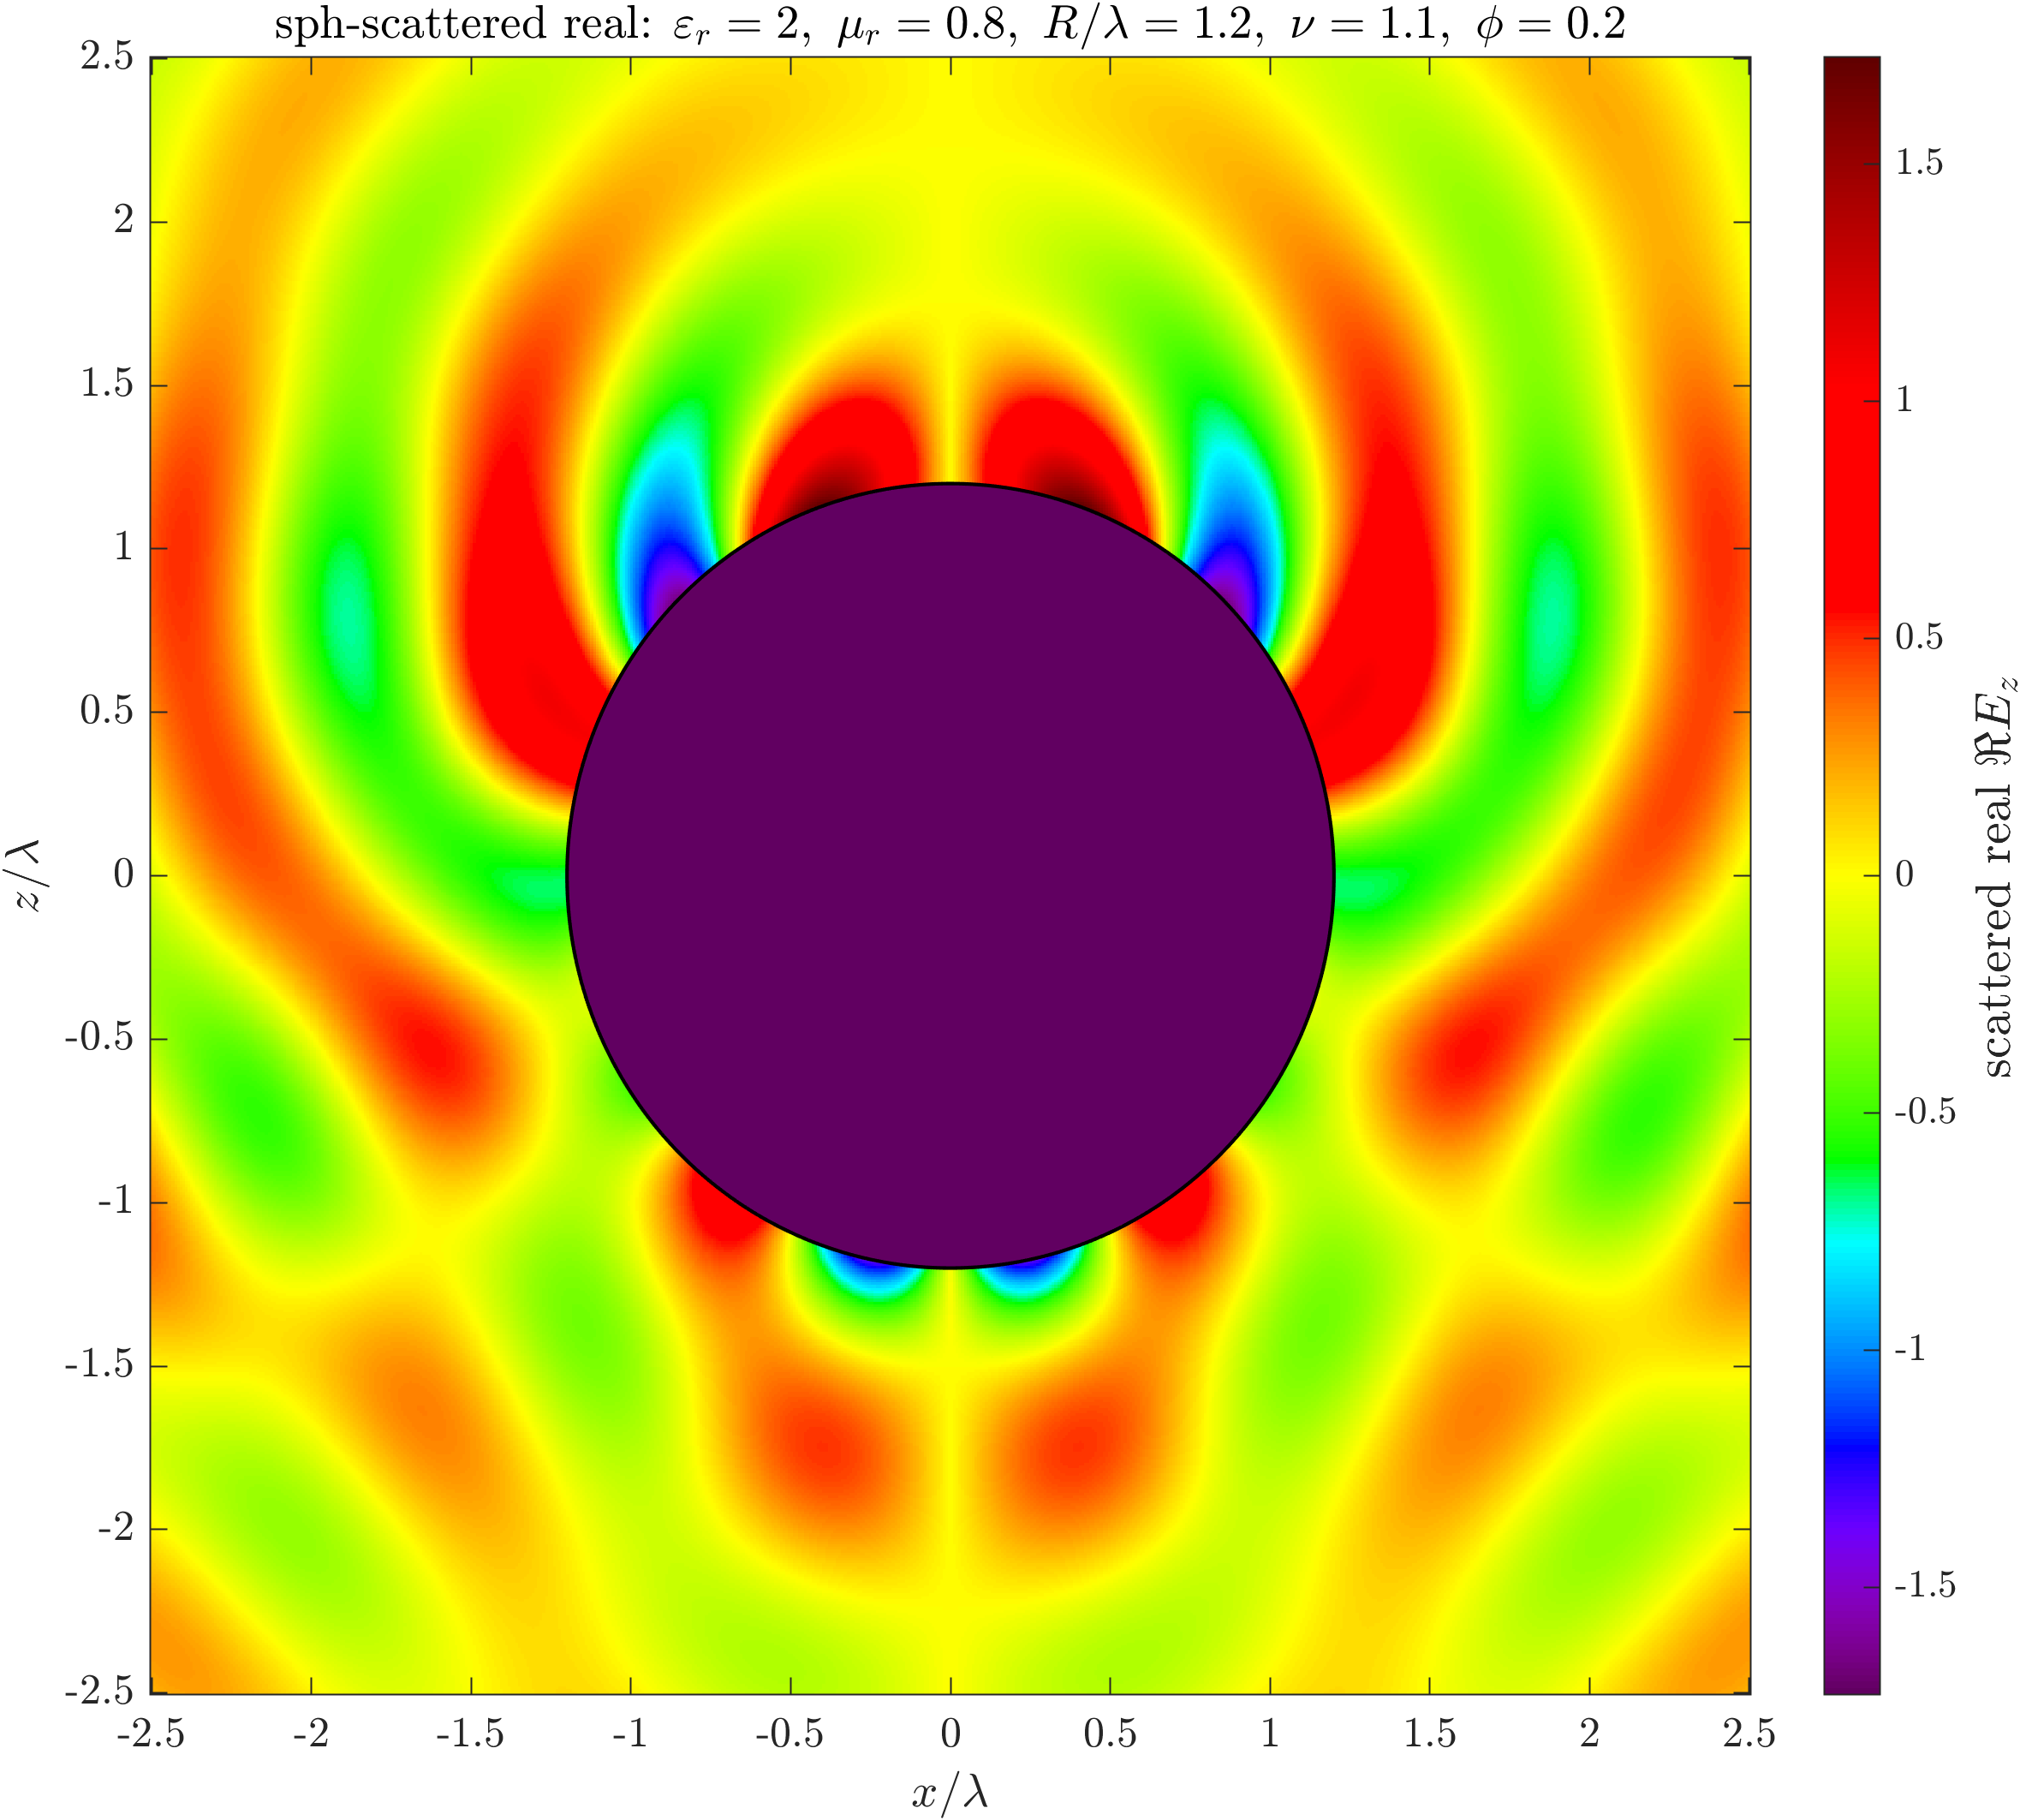
\includegraphics[width=\linewidth]{scattering_fig/lossless_large_sphere_z_direction_real_part.png}
			\caption{无损大球，\(z\)方向实部}
			\label{球体散射振幅比较图(对比有无损耗及不同半径)-无损大球,z方向实部}
		\end{subfigure}
		\hfill
		\begin{subfigure}{0.235\textwidth}
			\centering
			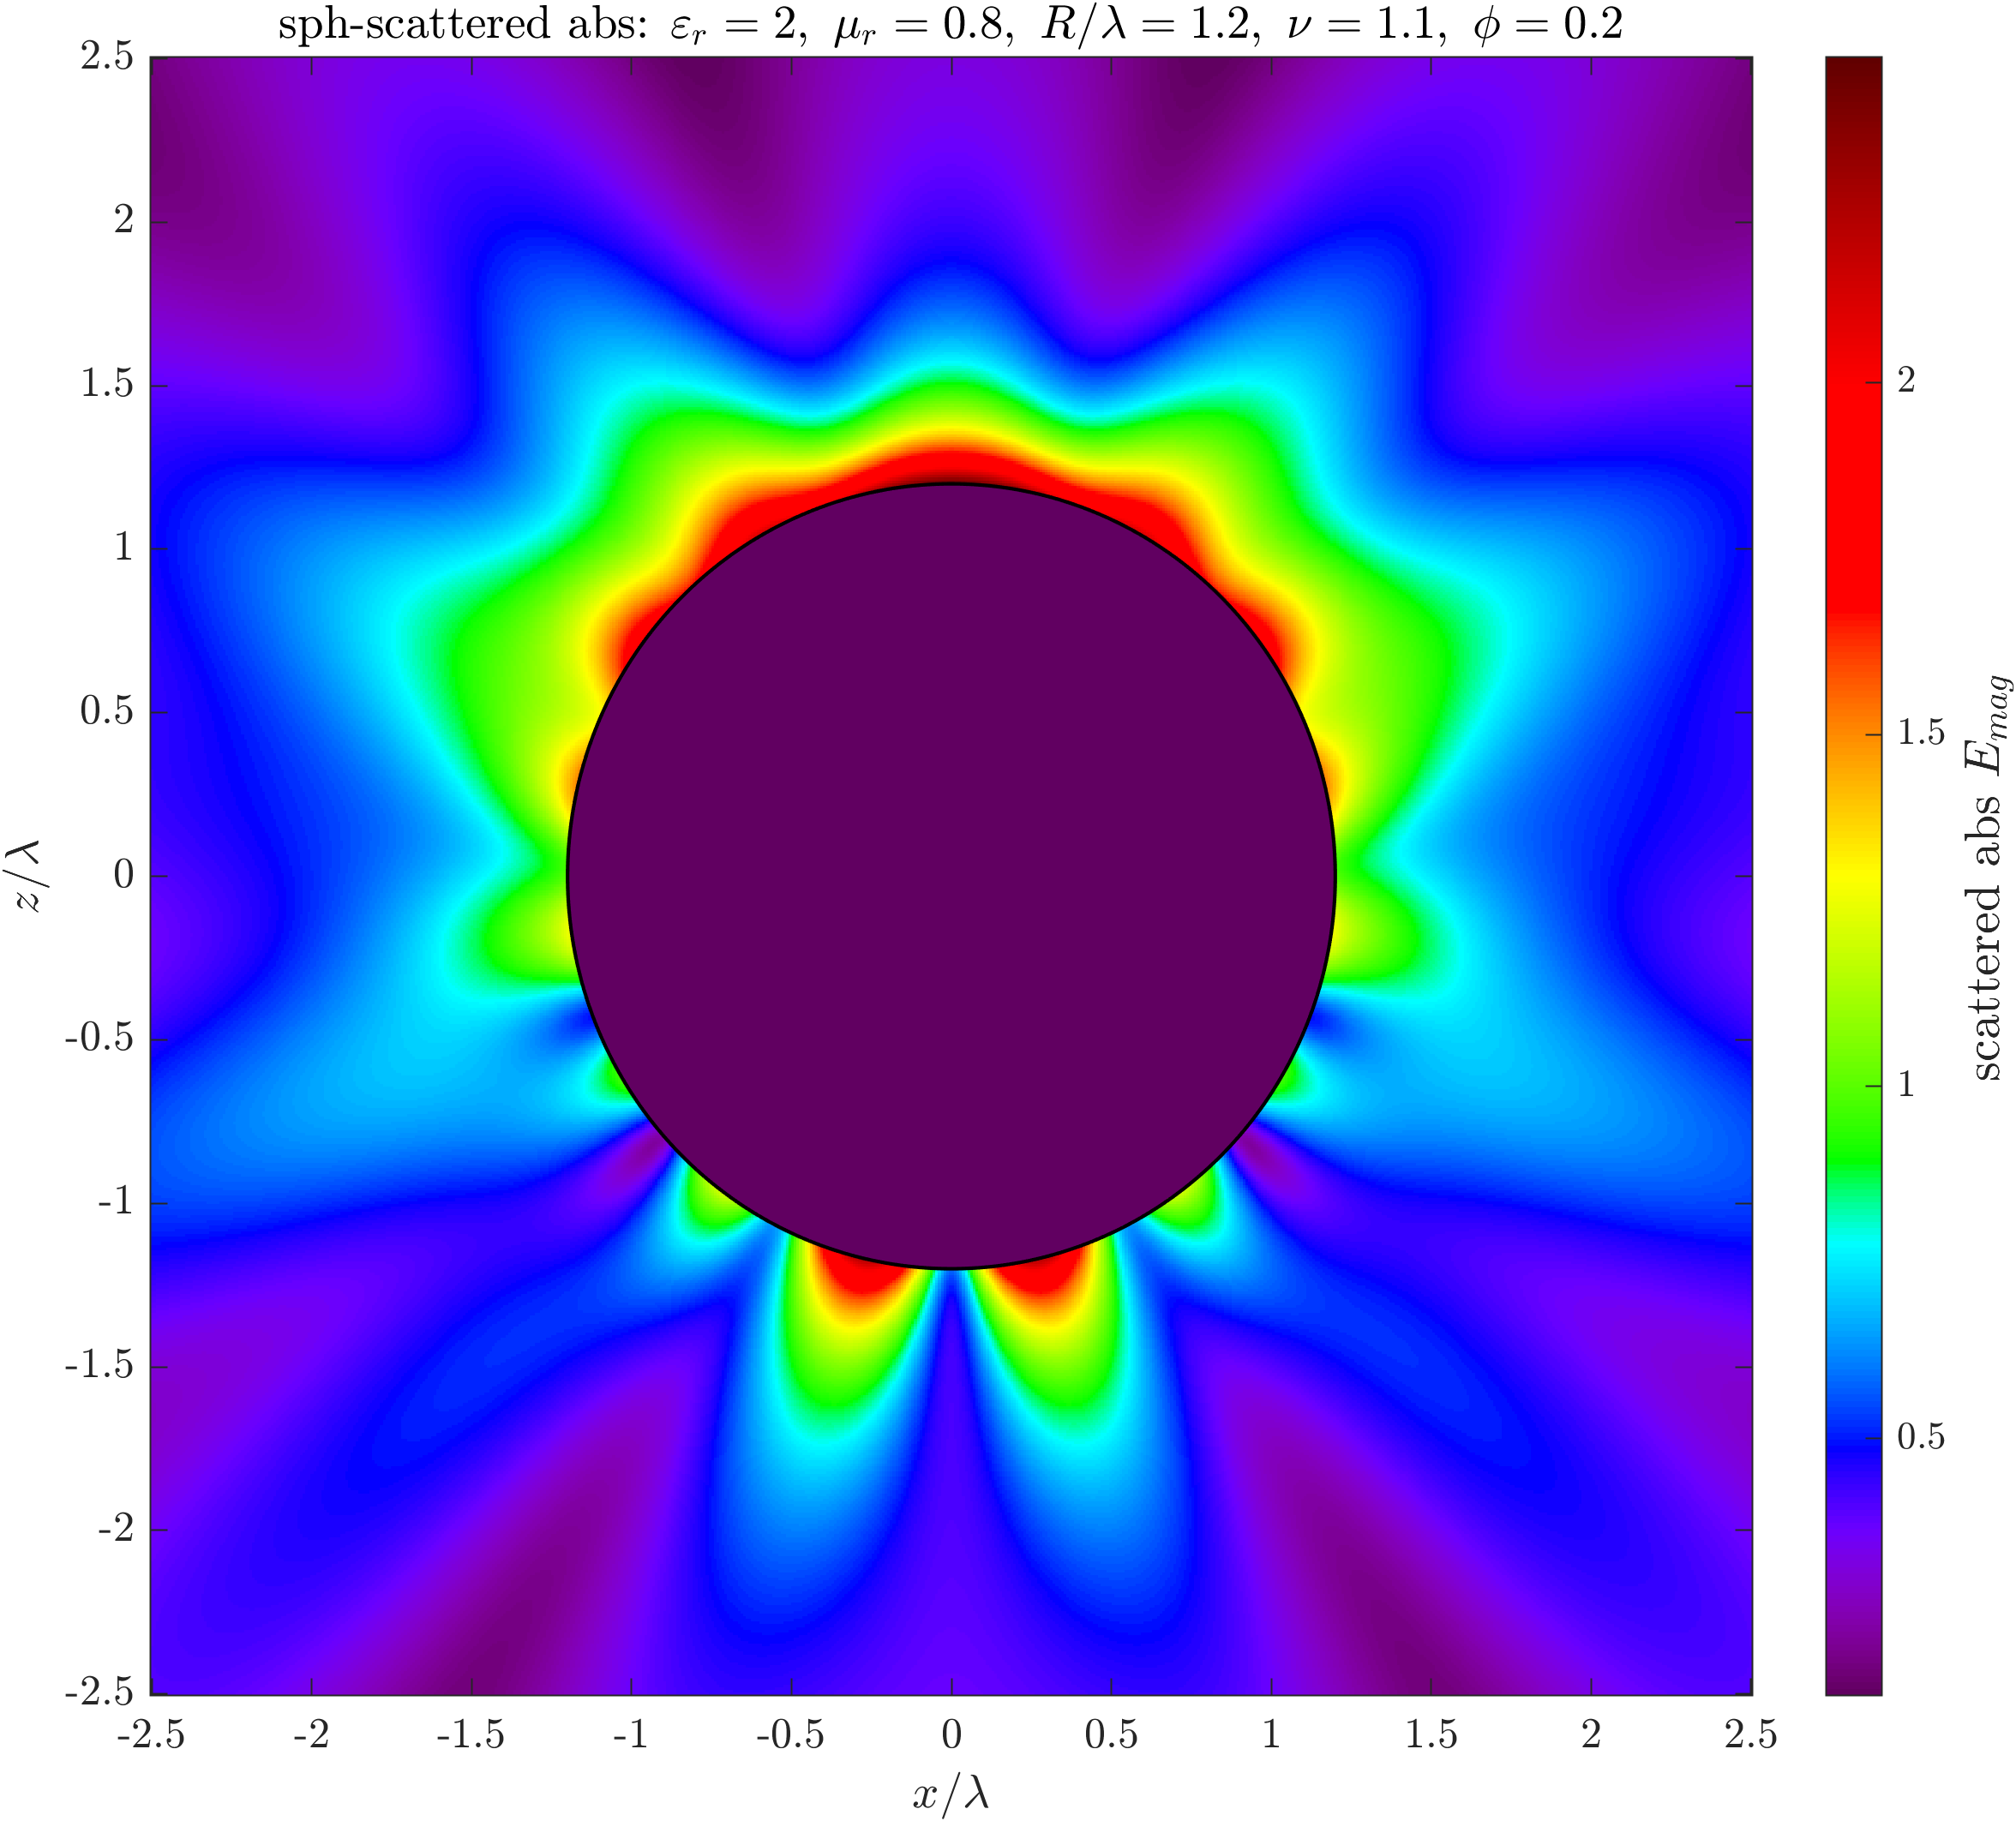
\includegraphics[width=\linewidth]{scattering_fig/lossless_large_sphere_amplitude_magnitude.png}
			\caption{无损大球，振幅大小}
			\label{球体散射振幅比较图(对比有无损耗及不同半径)-无损大球,振幅大小}
		\end{subfigure}

		\caption{球体散射振幅比较图（对比有无损耗及不同半径）}
		\label{球体散射振幅比较图(对比有无损耗及不同半径)}
		\label{fig:sphere-scattering-comparison-loss}
	\end{figure}

	% 第二个图：球体总场振幅比较图（一行，三个图）
	\begin{figure}[H]
		\centering
		% 第一个：有损小球总场振幅
		\begin{subfigure}{0.3\textwidth}
			\centering
			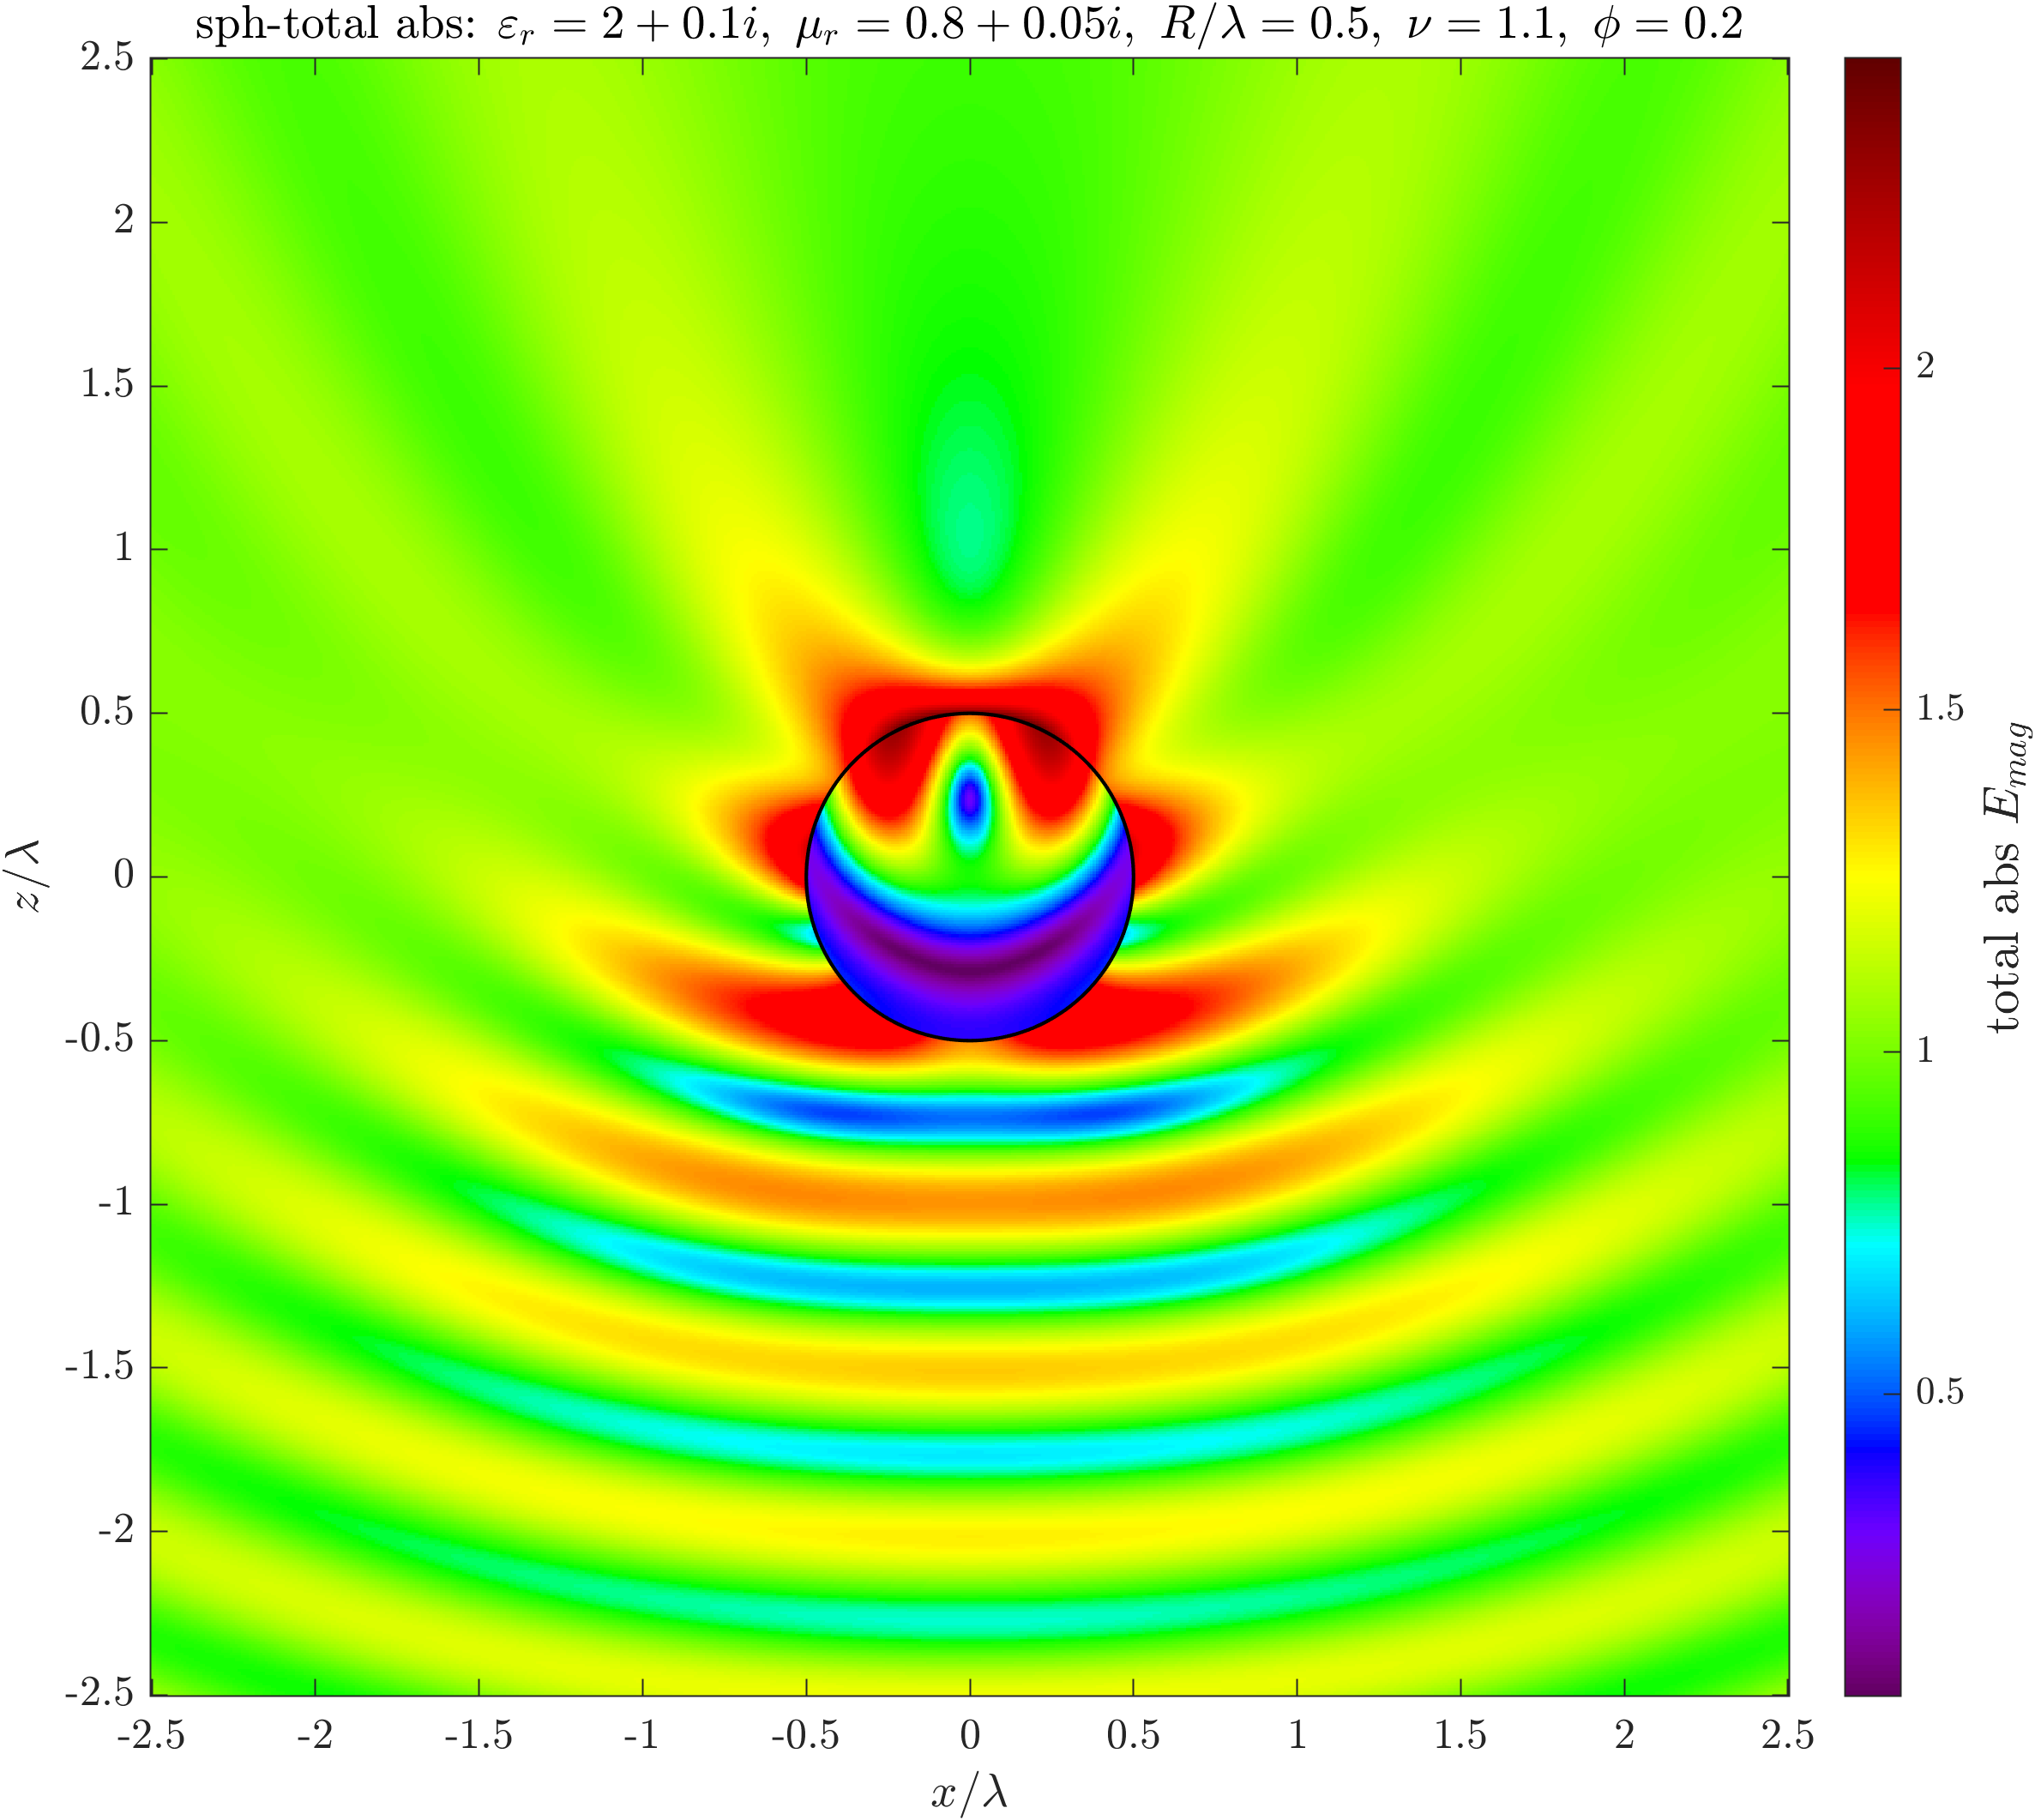
\includegraphics[width=\linewidth]{scattering_fig/lossy_small_sphere.png}
			\caption{有损小球}
			\label{球体总场振幅比较图(对比有无损耗及不同半径)-有损小球}
		\end{subfigure}
		\hfill
		% 第二个：有损大球总场振幅
		\begin{subfigure}{0.3\textwidth}
			\centering
			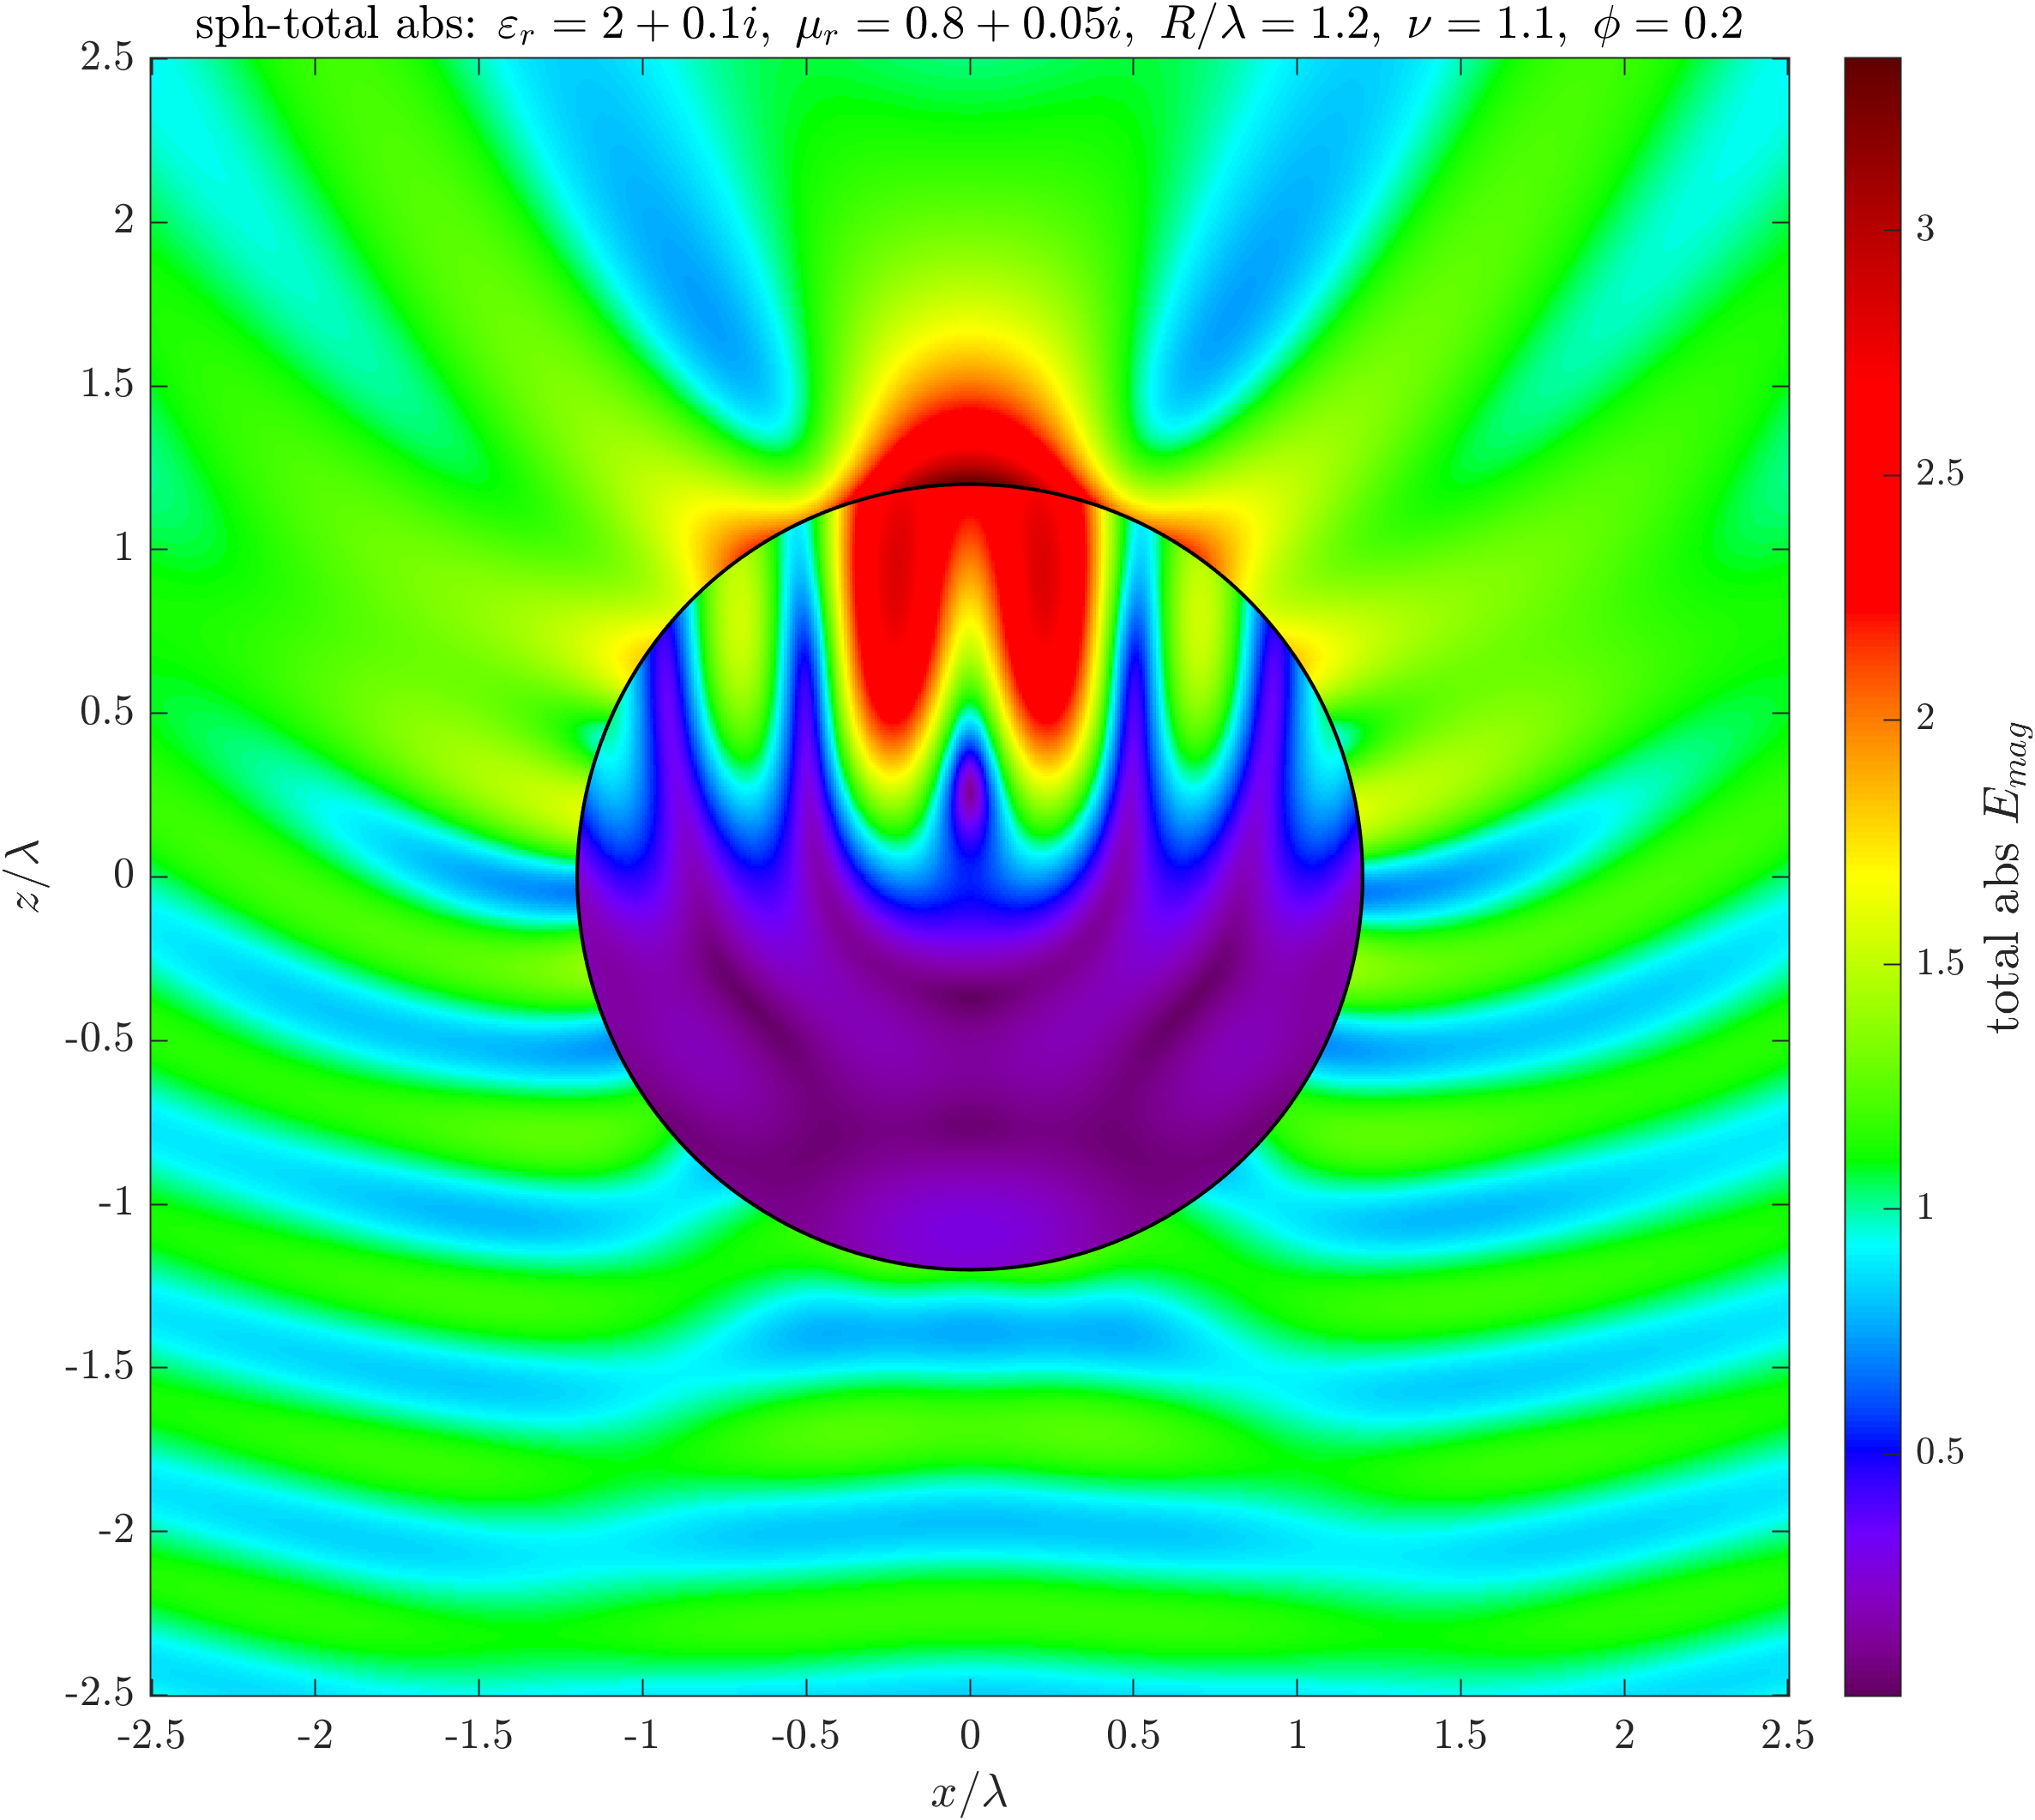
\includegraphics[width=\linewidth]{scattering_fig/lossy_large_sphere.png}
			\caption{有损大球}
			\label{球体总场振幅比较图(对比有无损耗及不同半径)-有损大球}
		\end{subfigure}
		\hfill
		% 第三个：无损大球总场振幅
		\begin{subfigure}{0.3\textwidth}
			\centering
			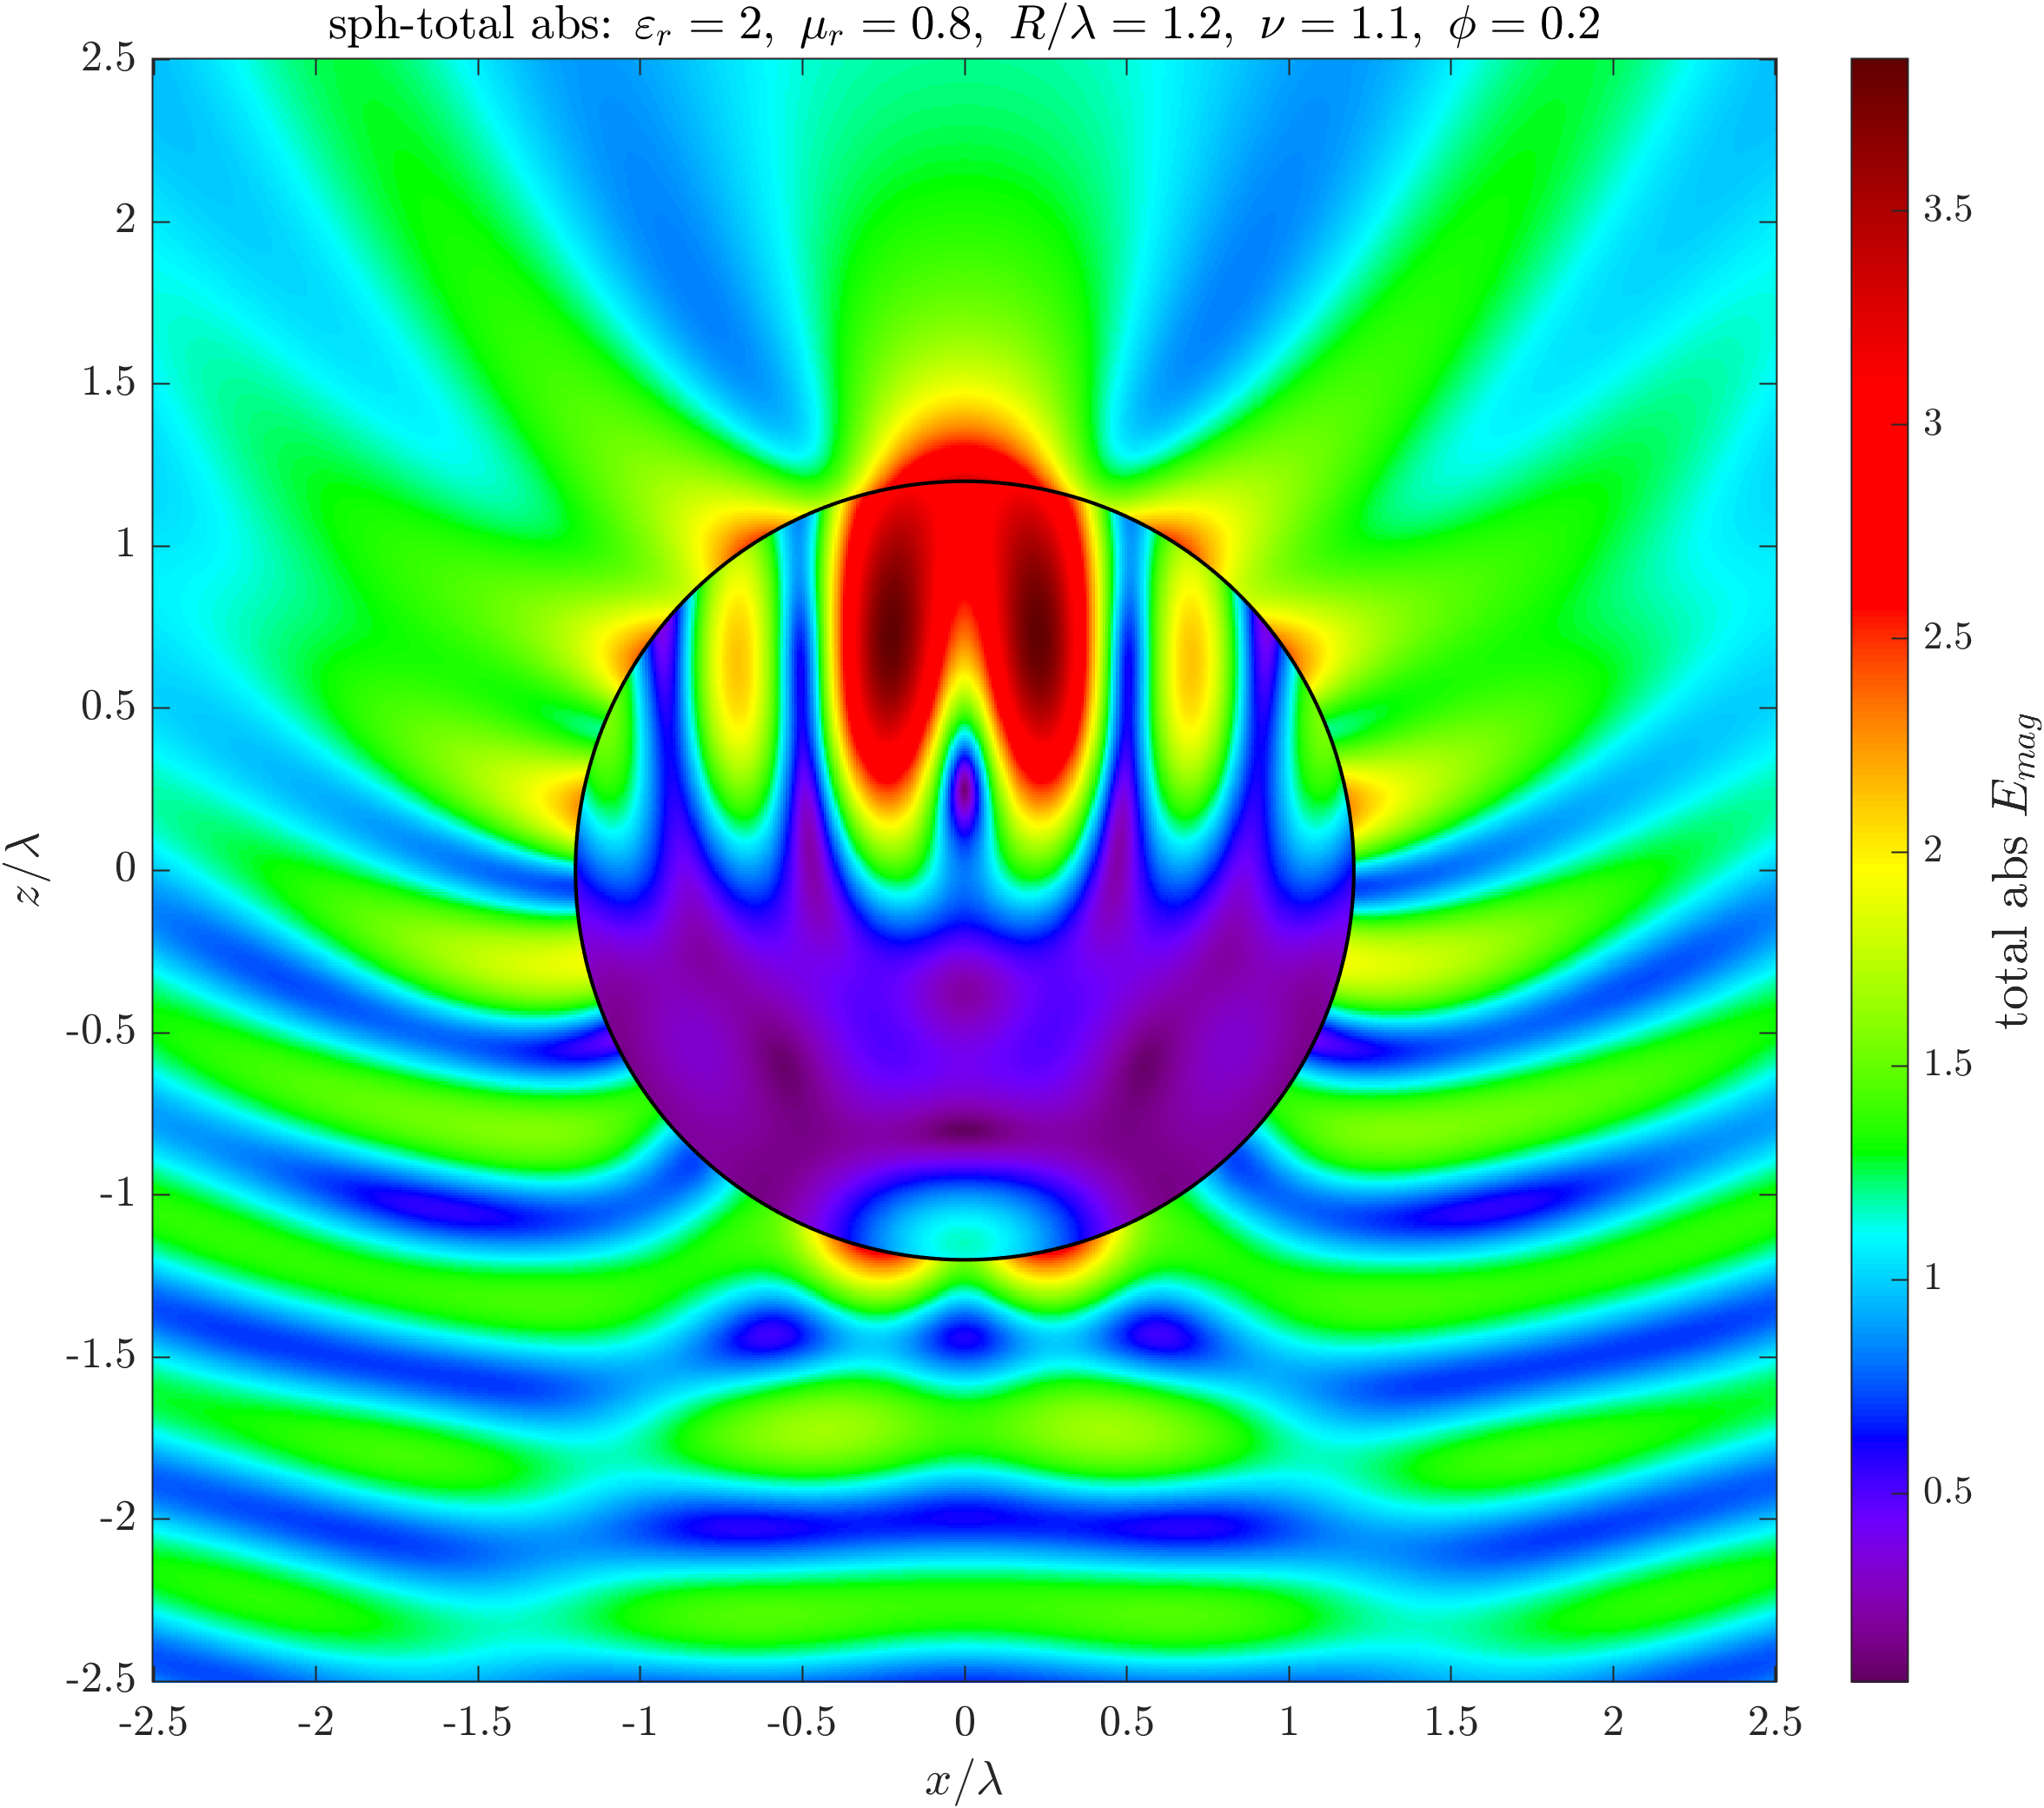
\includegraphics[width=\linewidth]{scattering_fig/lossless_large_sphere.png}
			\caption{无损大球}
			\label{球体总场振幅比较图(对比有无损耗及不同半径)-无损大球}
		\end{subfigure}

		\caption{球体总场振幅比较图（对比有无损耗及不同半径）}
		\label{球体总场振幅比较图(对比有无损耗及不同半径)}
		\label{fig:sphere-total-comparison-loss}
	\end{figure}

	% 同理，如果需要柱体的类似对比，可以按照相同模式添加：
	% 柱体散射振幅比较图（三行，每行四个图）
	\begin{figure}[H]
		\centering
		% 第一行：有损小柱 (R/lambda=0.5, 有损耗)
		\begin{subfigure}{0.235\textwidth}
			\centering
			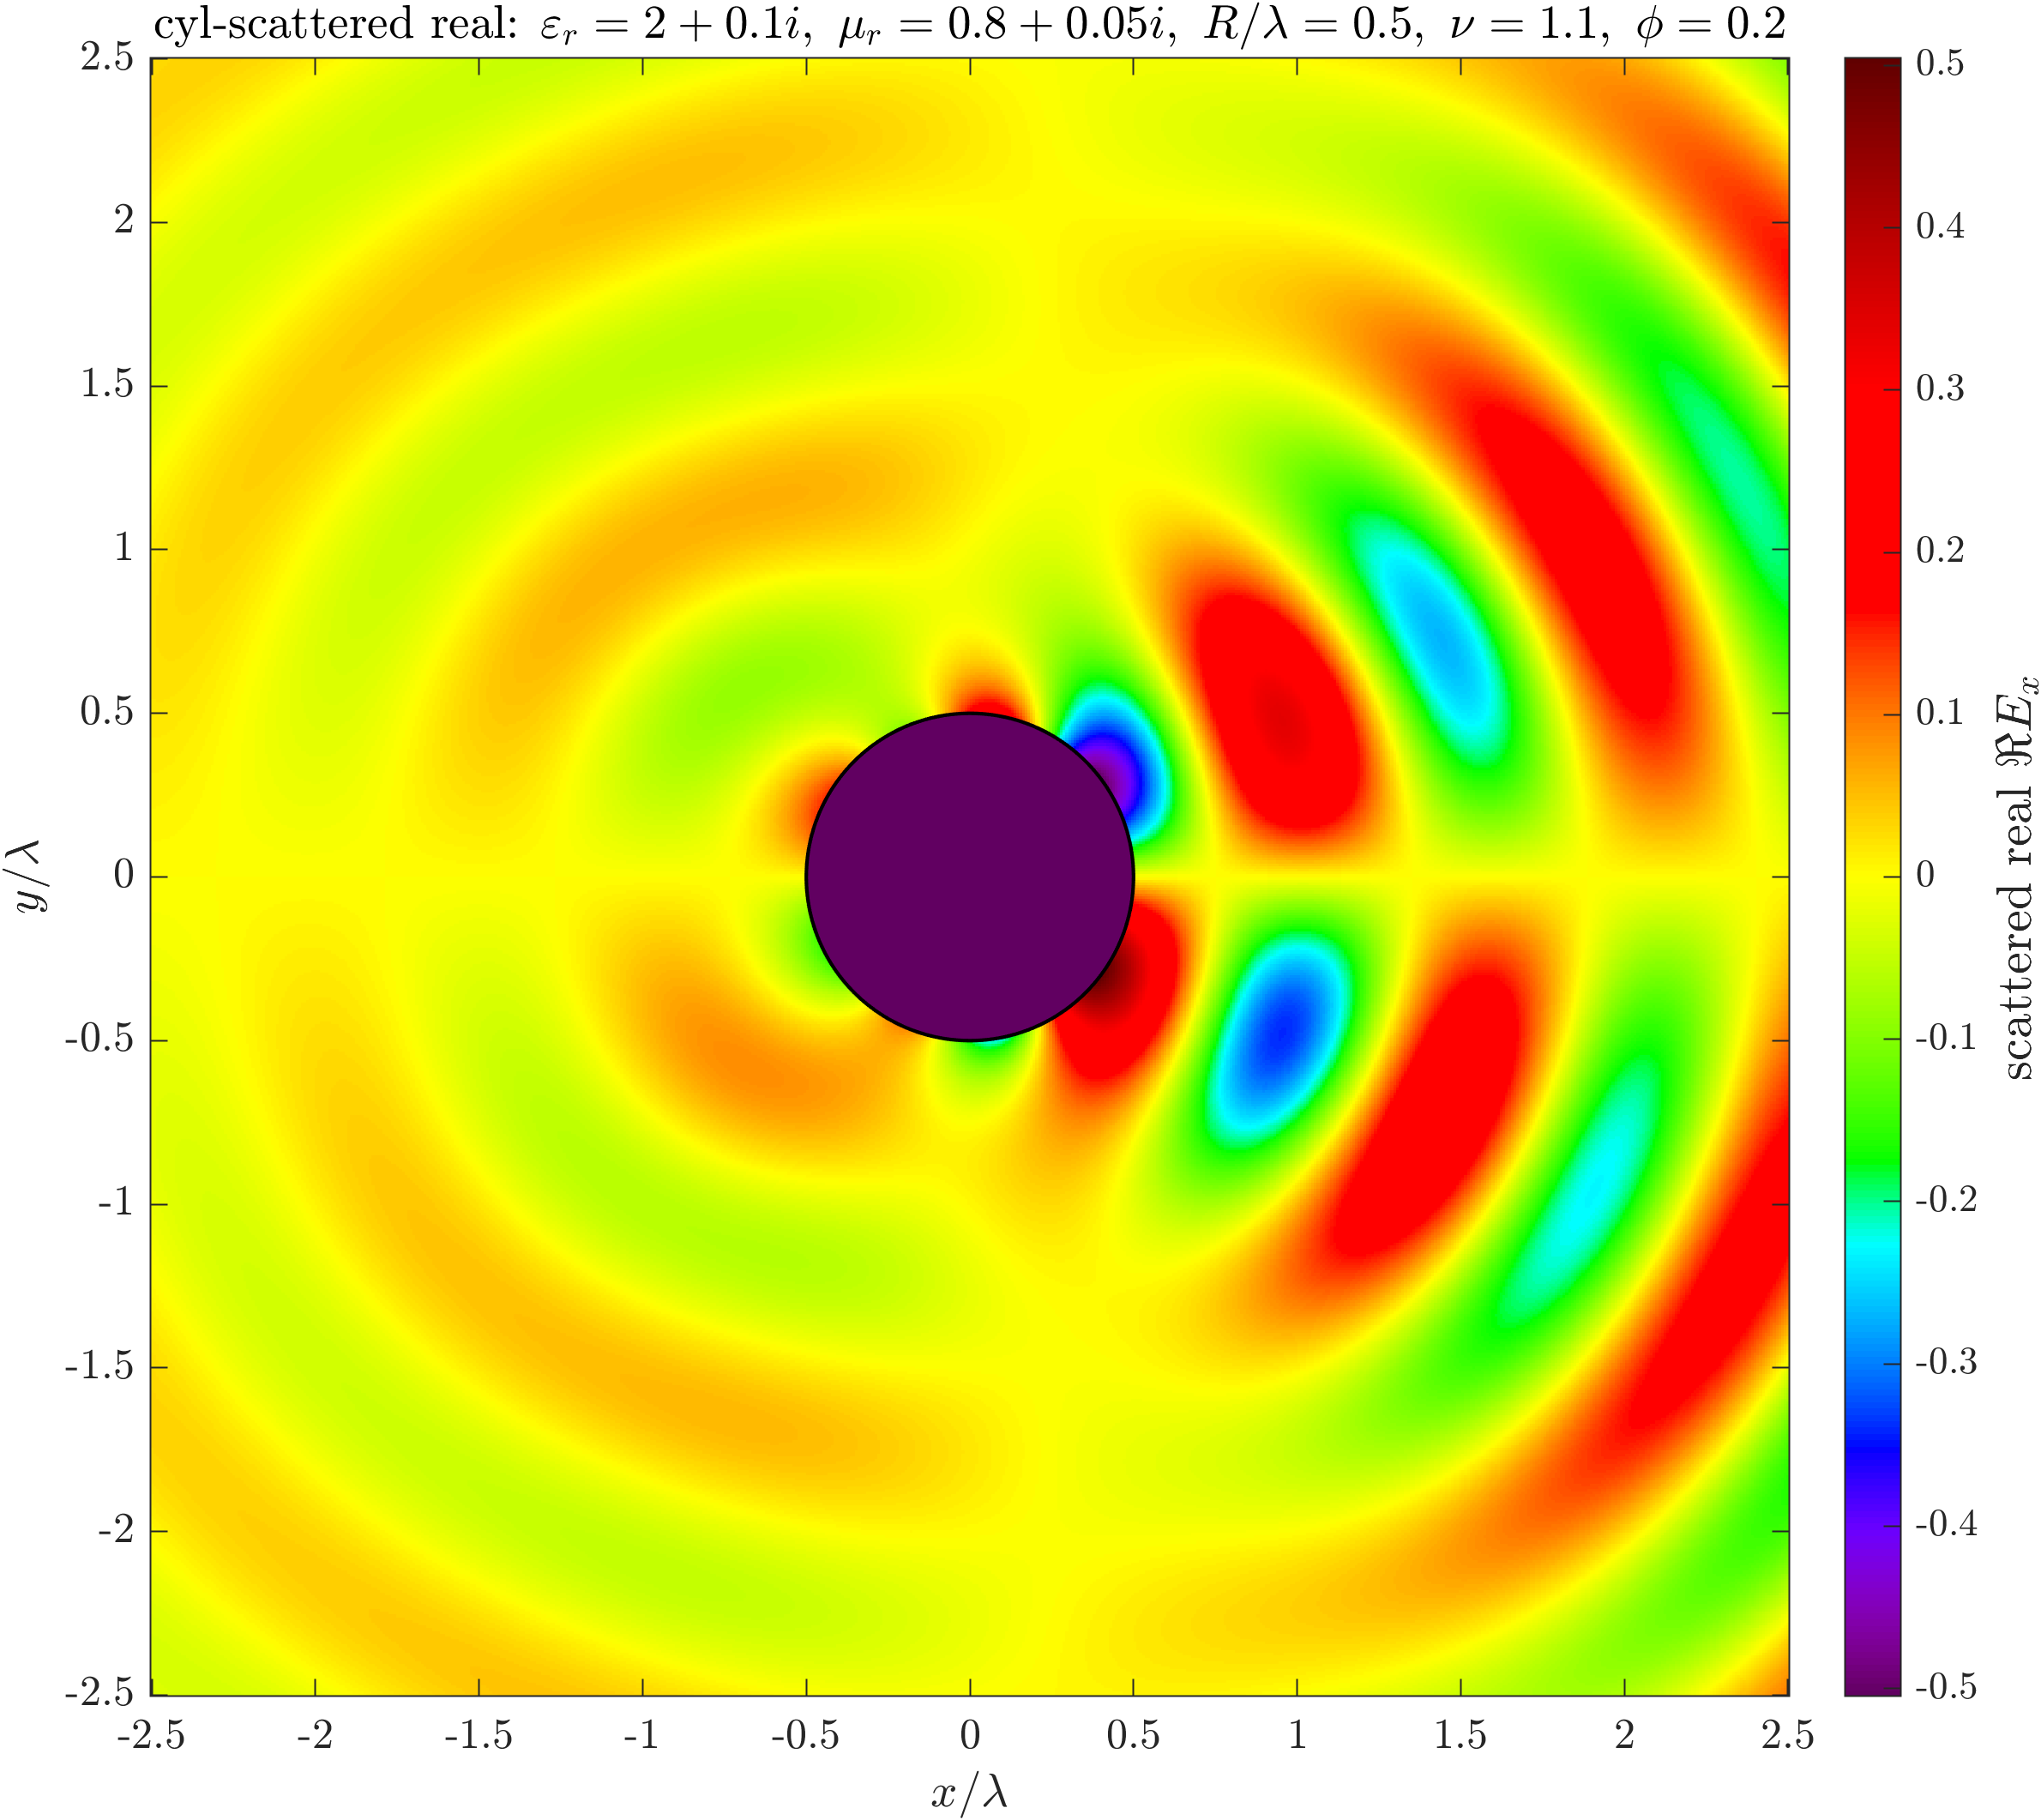
\includegraphics[width=\linewidth]{scattering_fig/lossy_small_cylinder_x_direction_real_part.png}
			\caption{有损小柱，\(x\)方向实部}
			\label{柱体散射振幅比较图(对比有无损耗及不同半径)-有损小柱,x方向实部}
		\end{subfigure}
		\hfill
		\begin{subfigure}{0.235\textwidth}
			\centering
			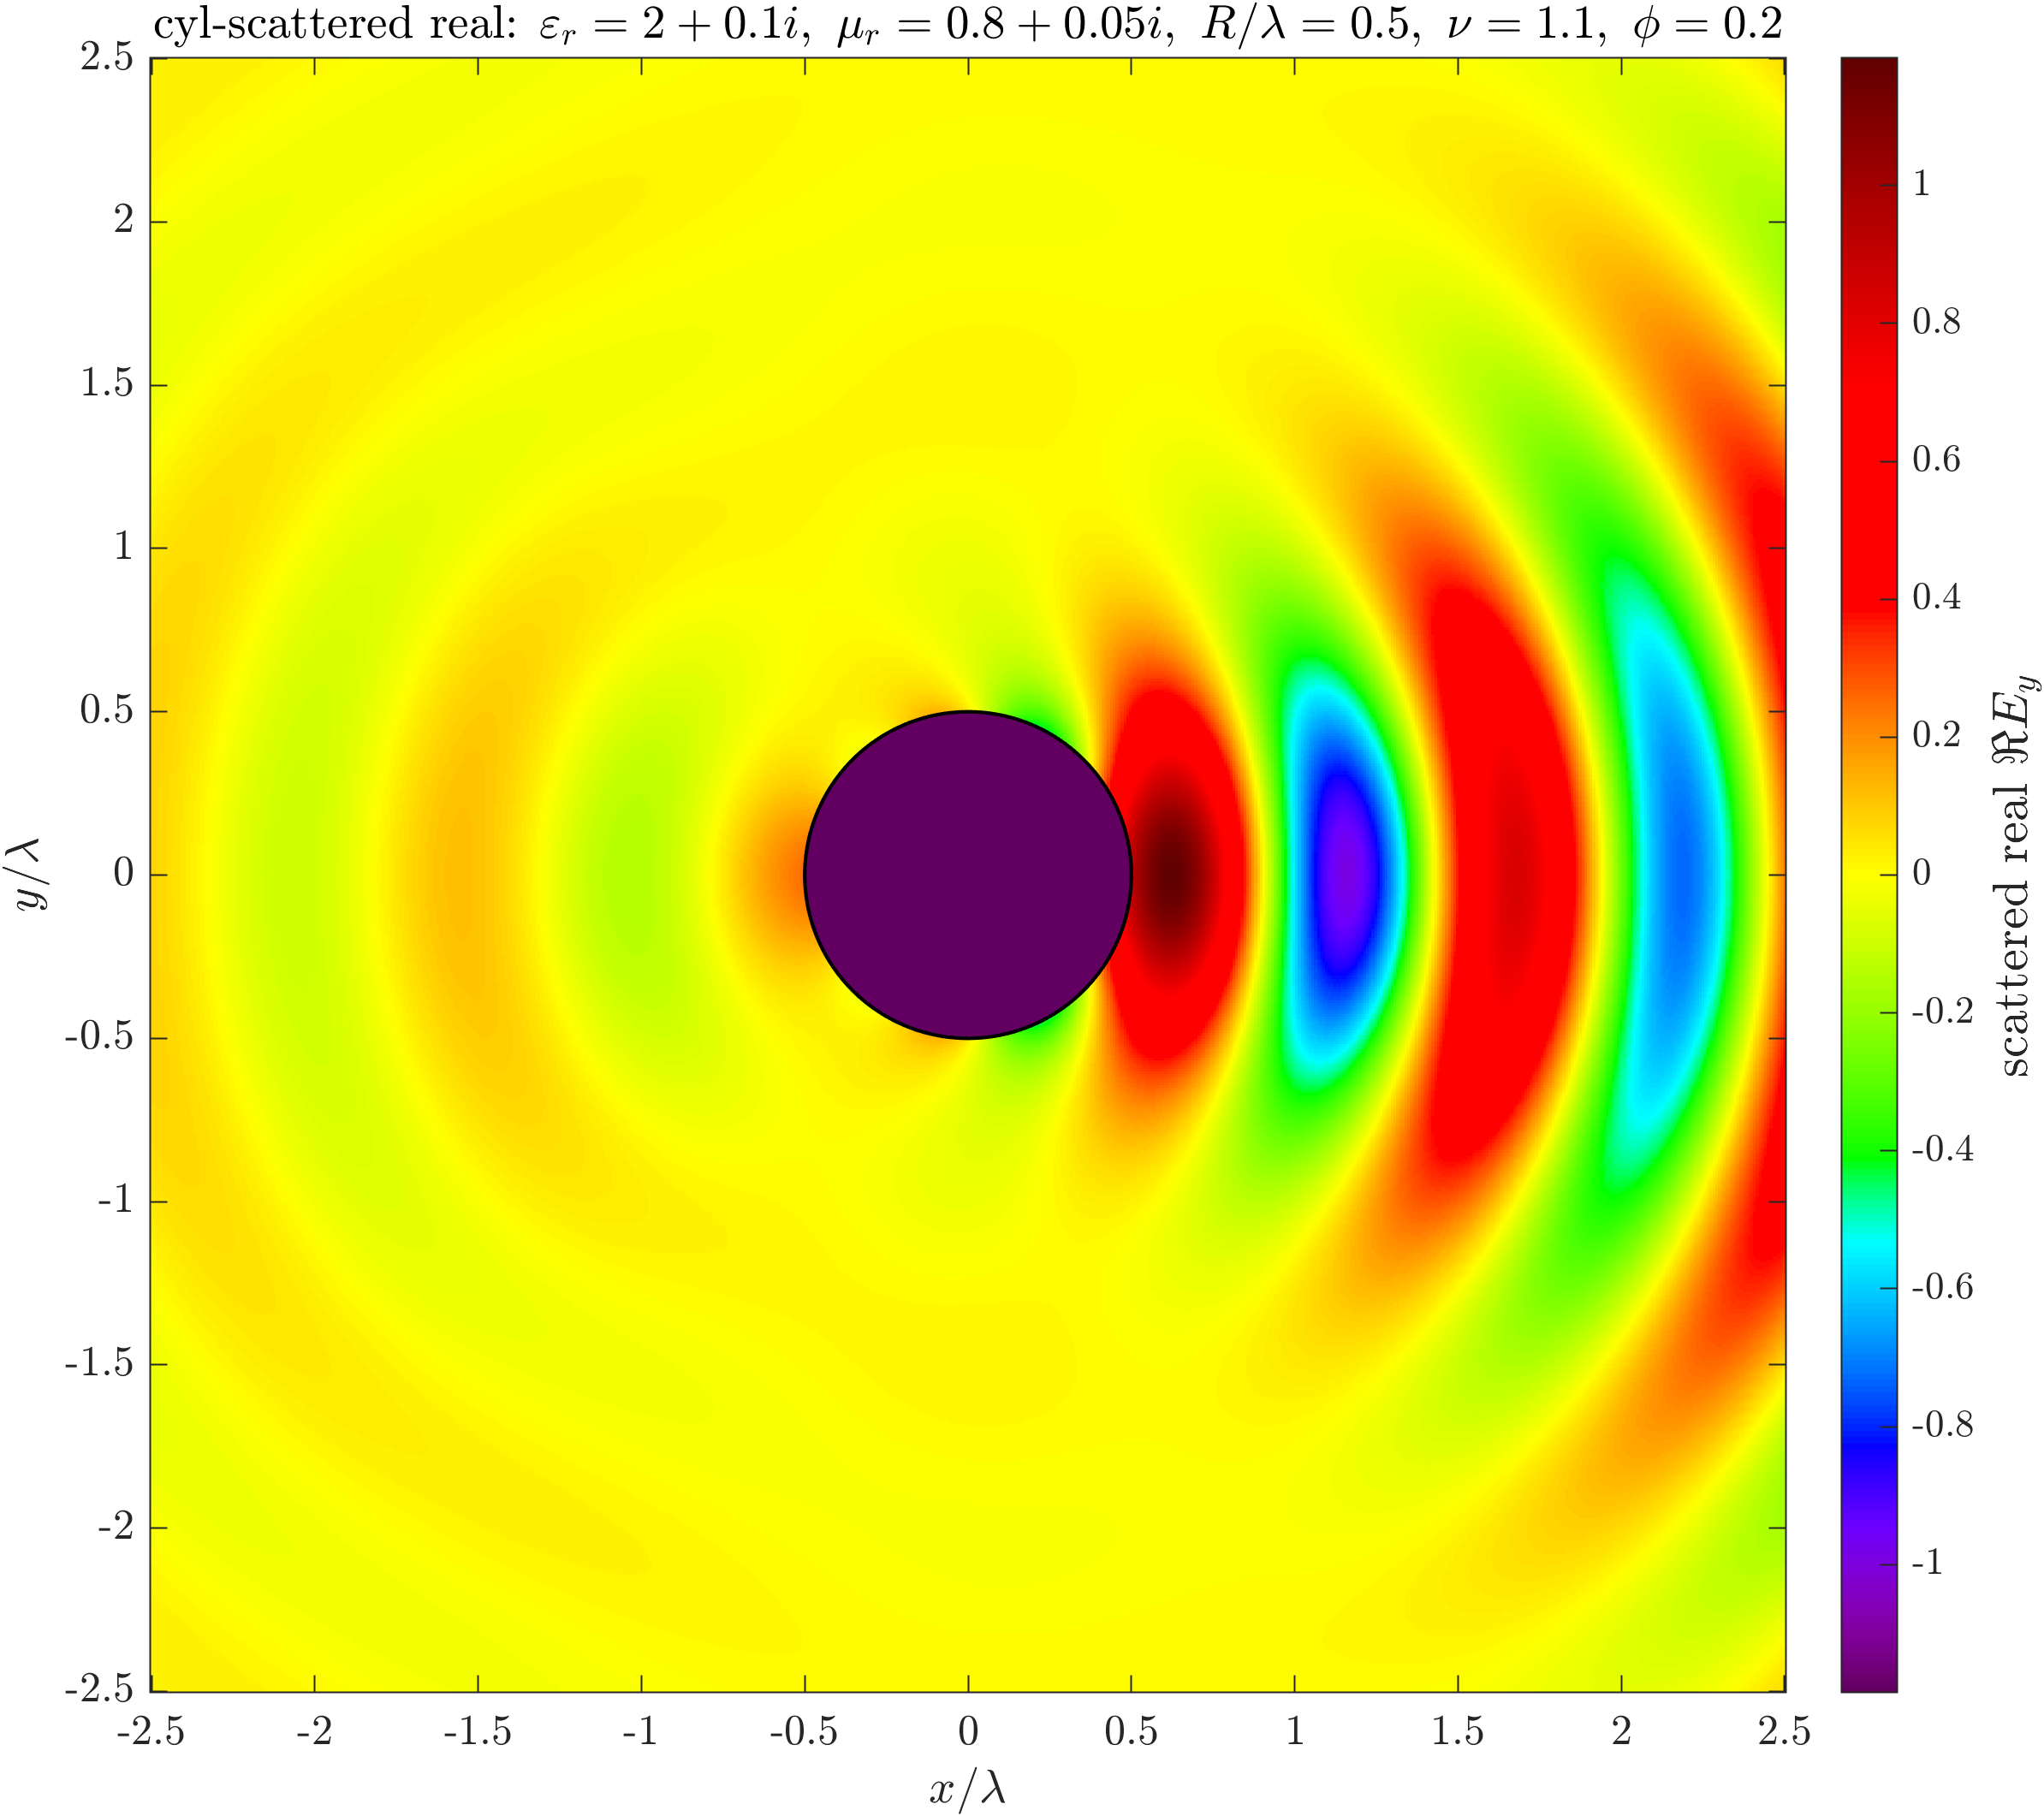
\includegraphics[width=\linewidth]{scattering_fig/lossy_small_cylinder_y_direction_real_part.png}
			\caption{有损小柱，\(y\)方向实部}
			\label{柱体散射振幅比较图(对比有无损耗及不同半径)-有损小柱,y方向实部}
		\end{subfigure}
		\hfill
		\begin{subfigure}{0.235\textwidth}
			\centering
			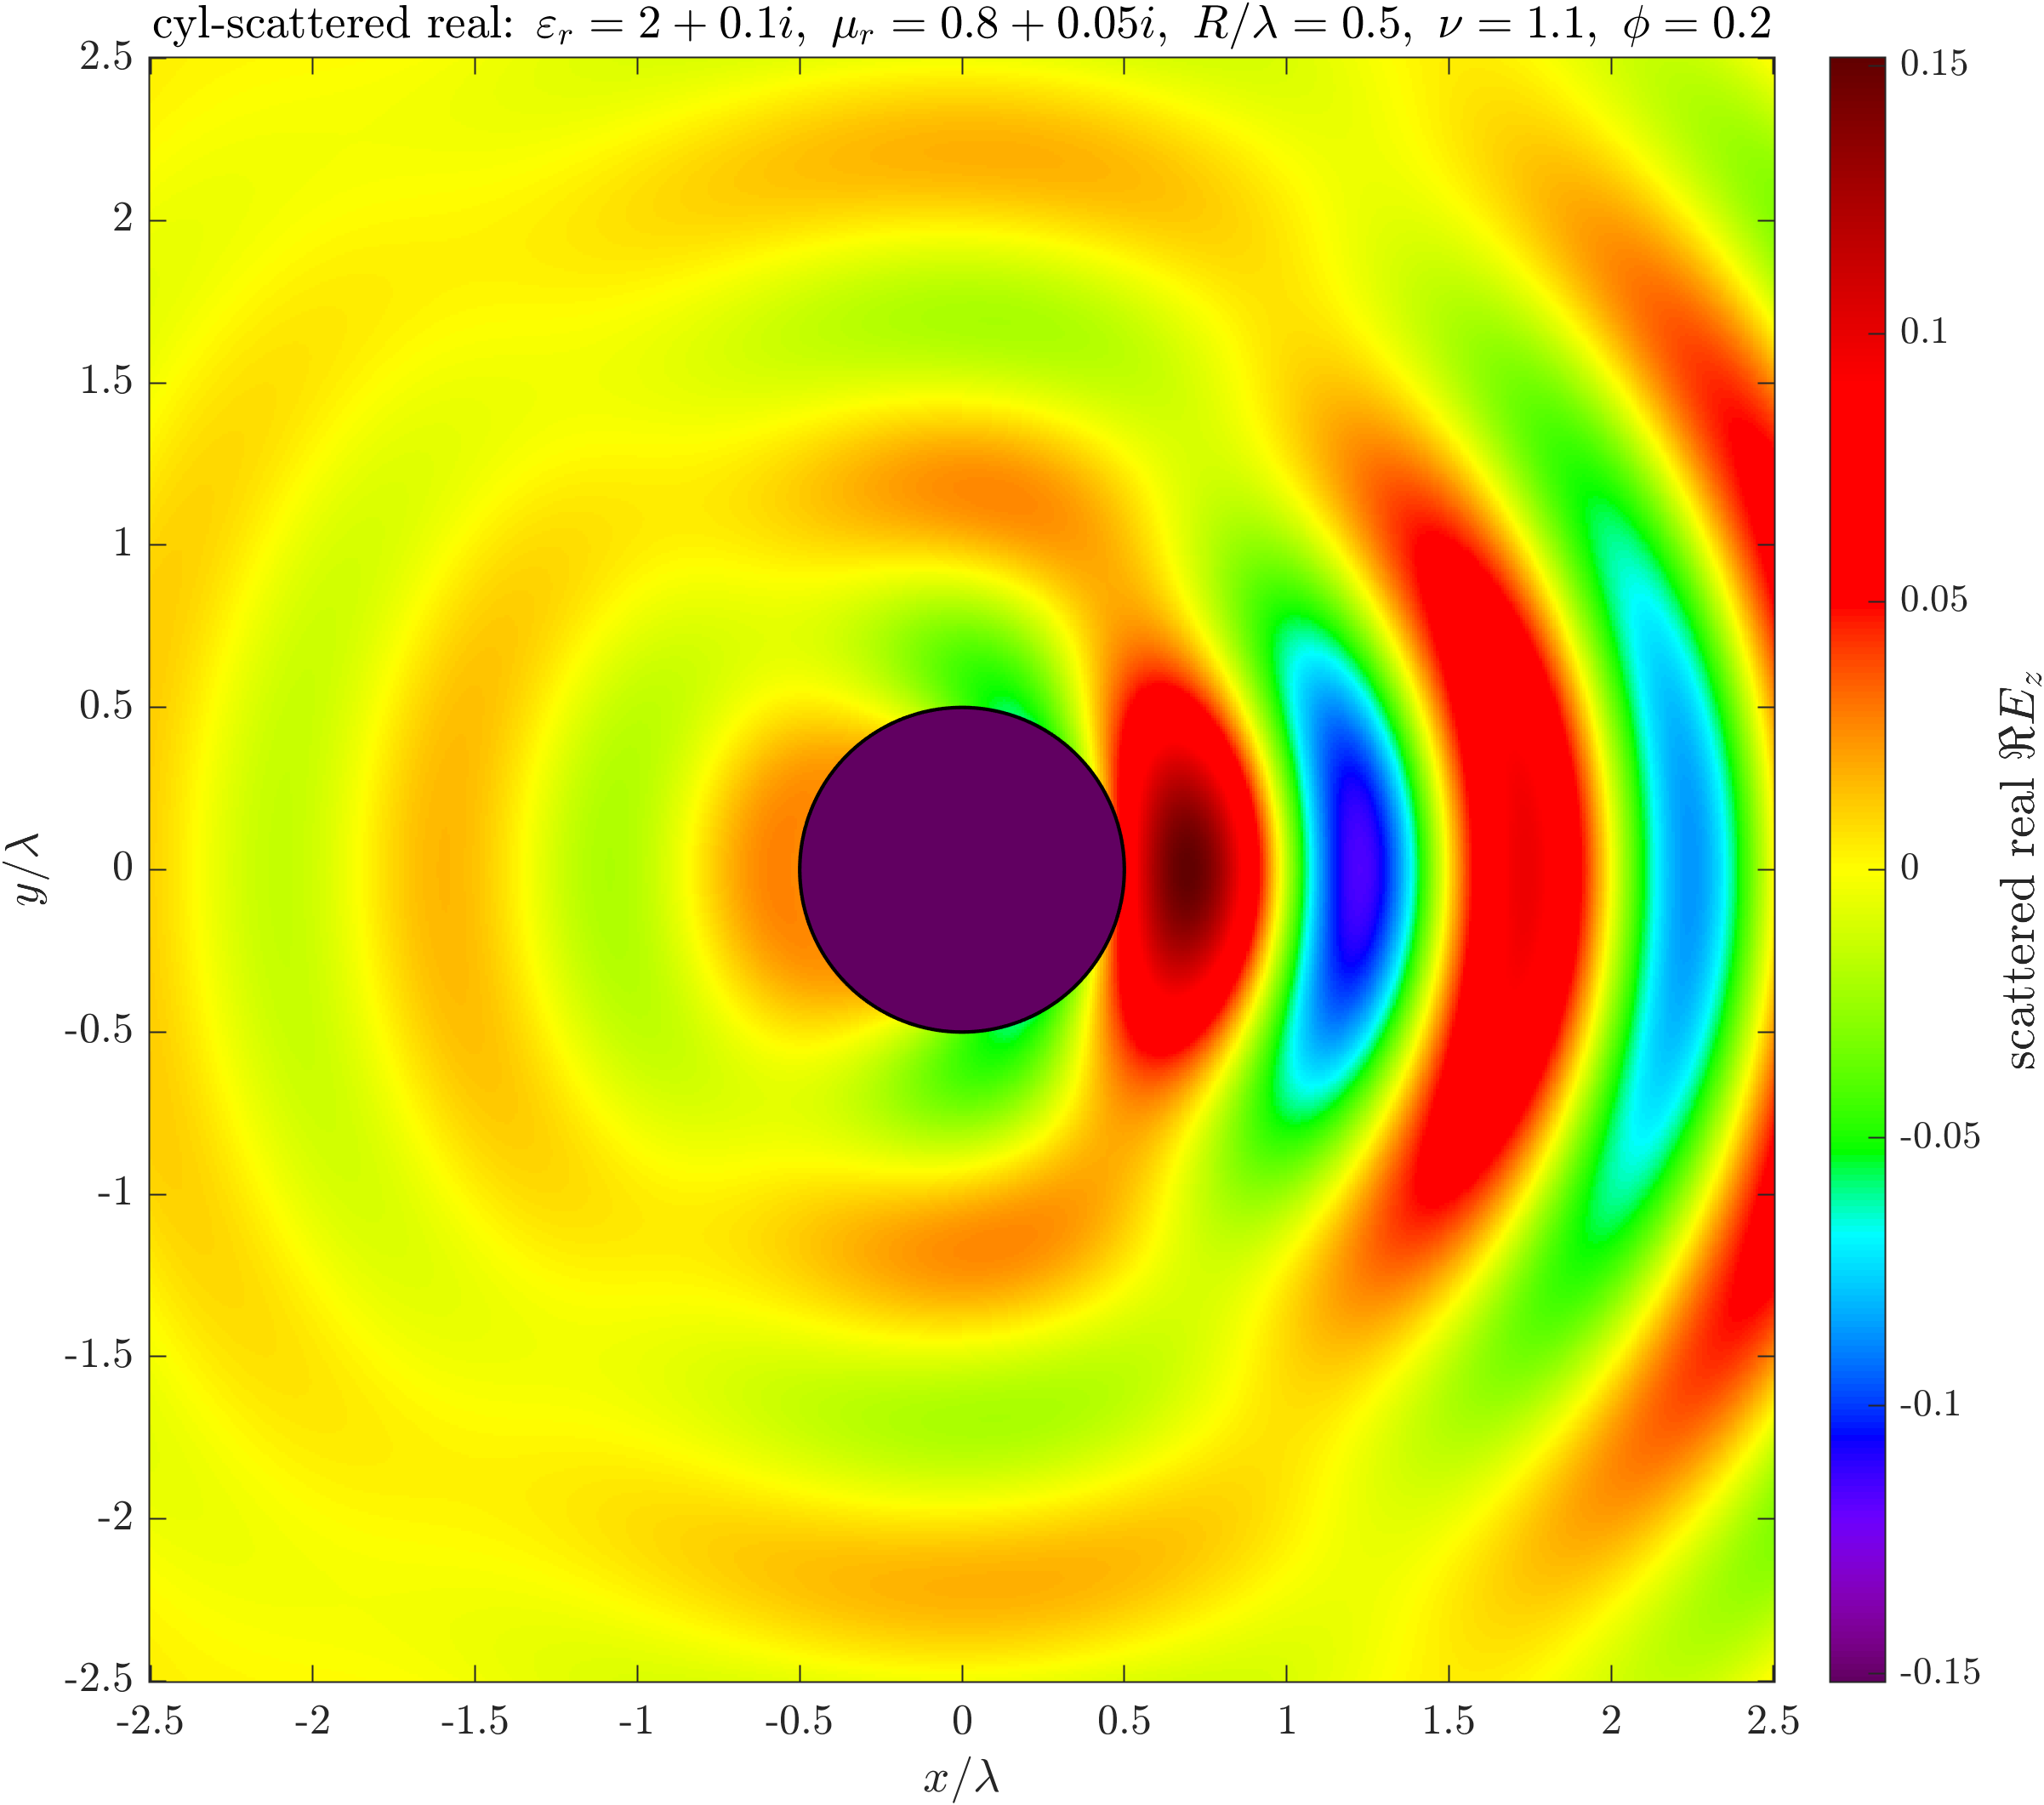
\includegraphics[width=\linewidth]{scattering_fig/lossy_small_cylinder_z_direction_real_part.png}
			\caption{有损小柱，\(z\)方向实部}
			\label{柱体散射振幅比较图(对比有无损耗及不同半径)-有损小柱,z方向实部}
		\end{subfigure}
		\hfill
		\begin{subfigure}{0.235\textwidth}
			\centering
			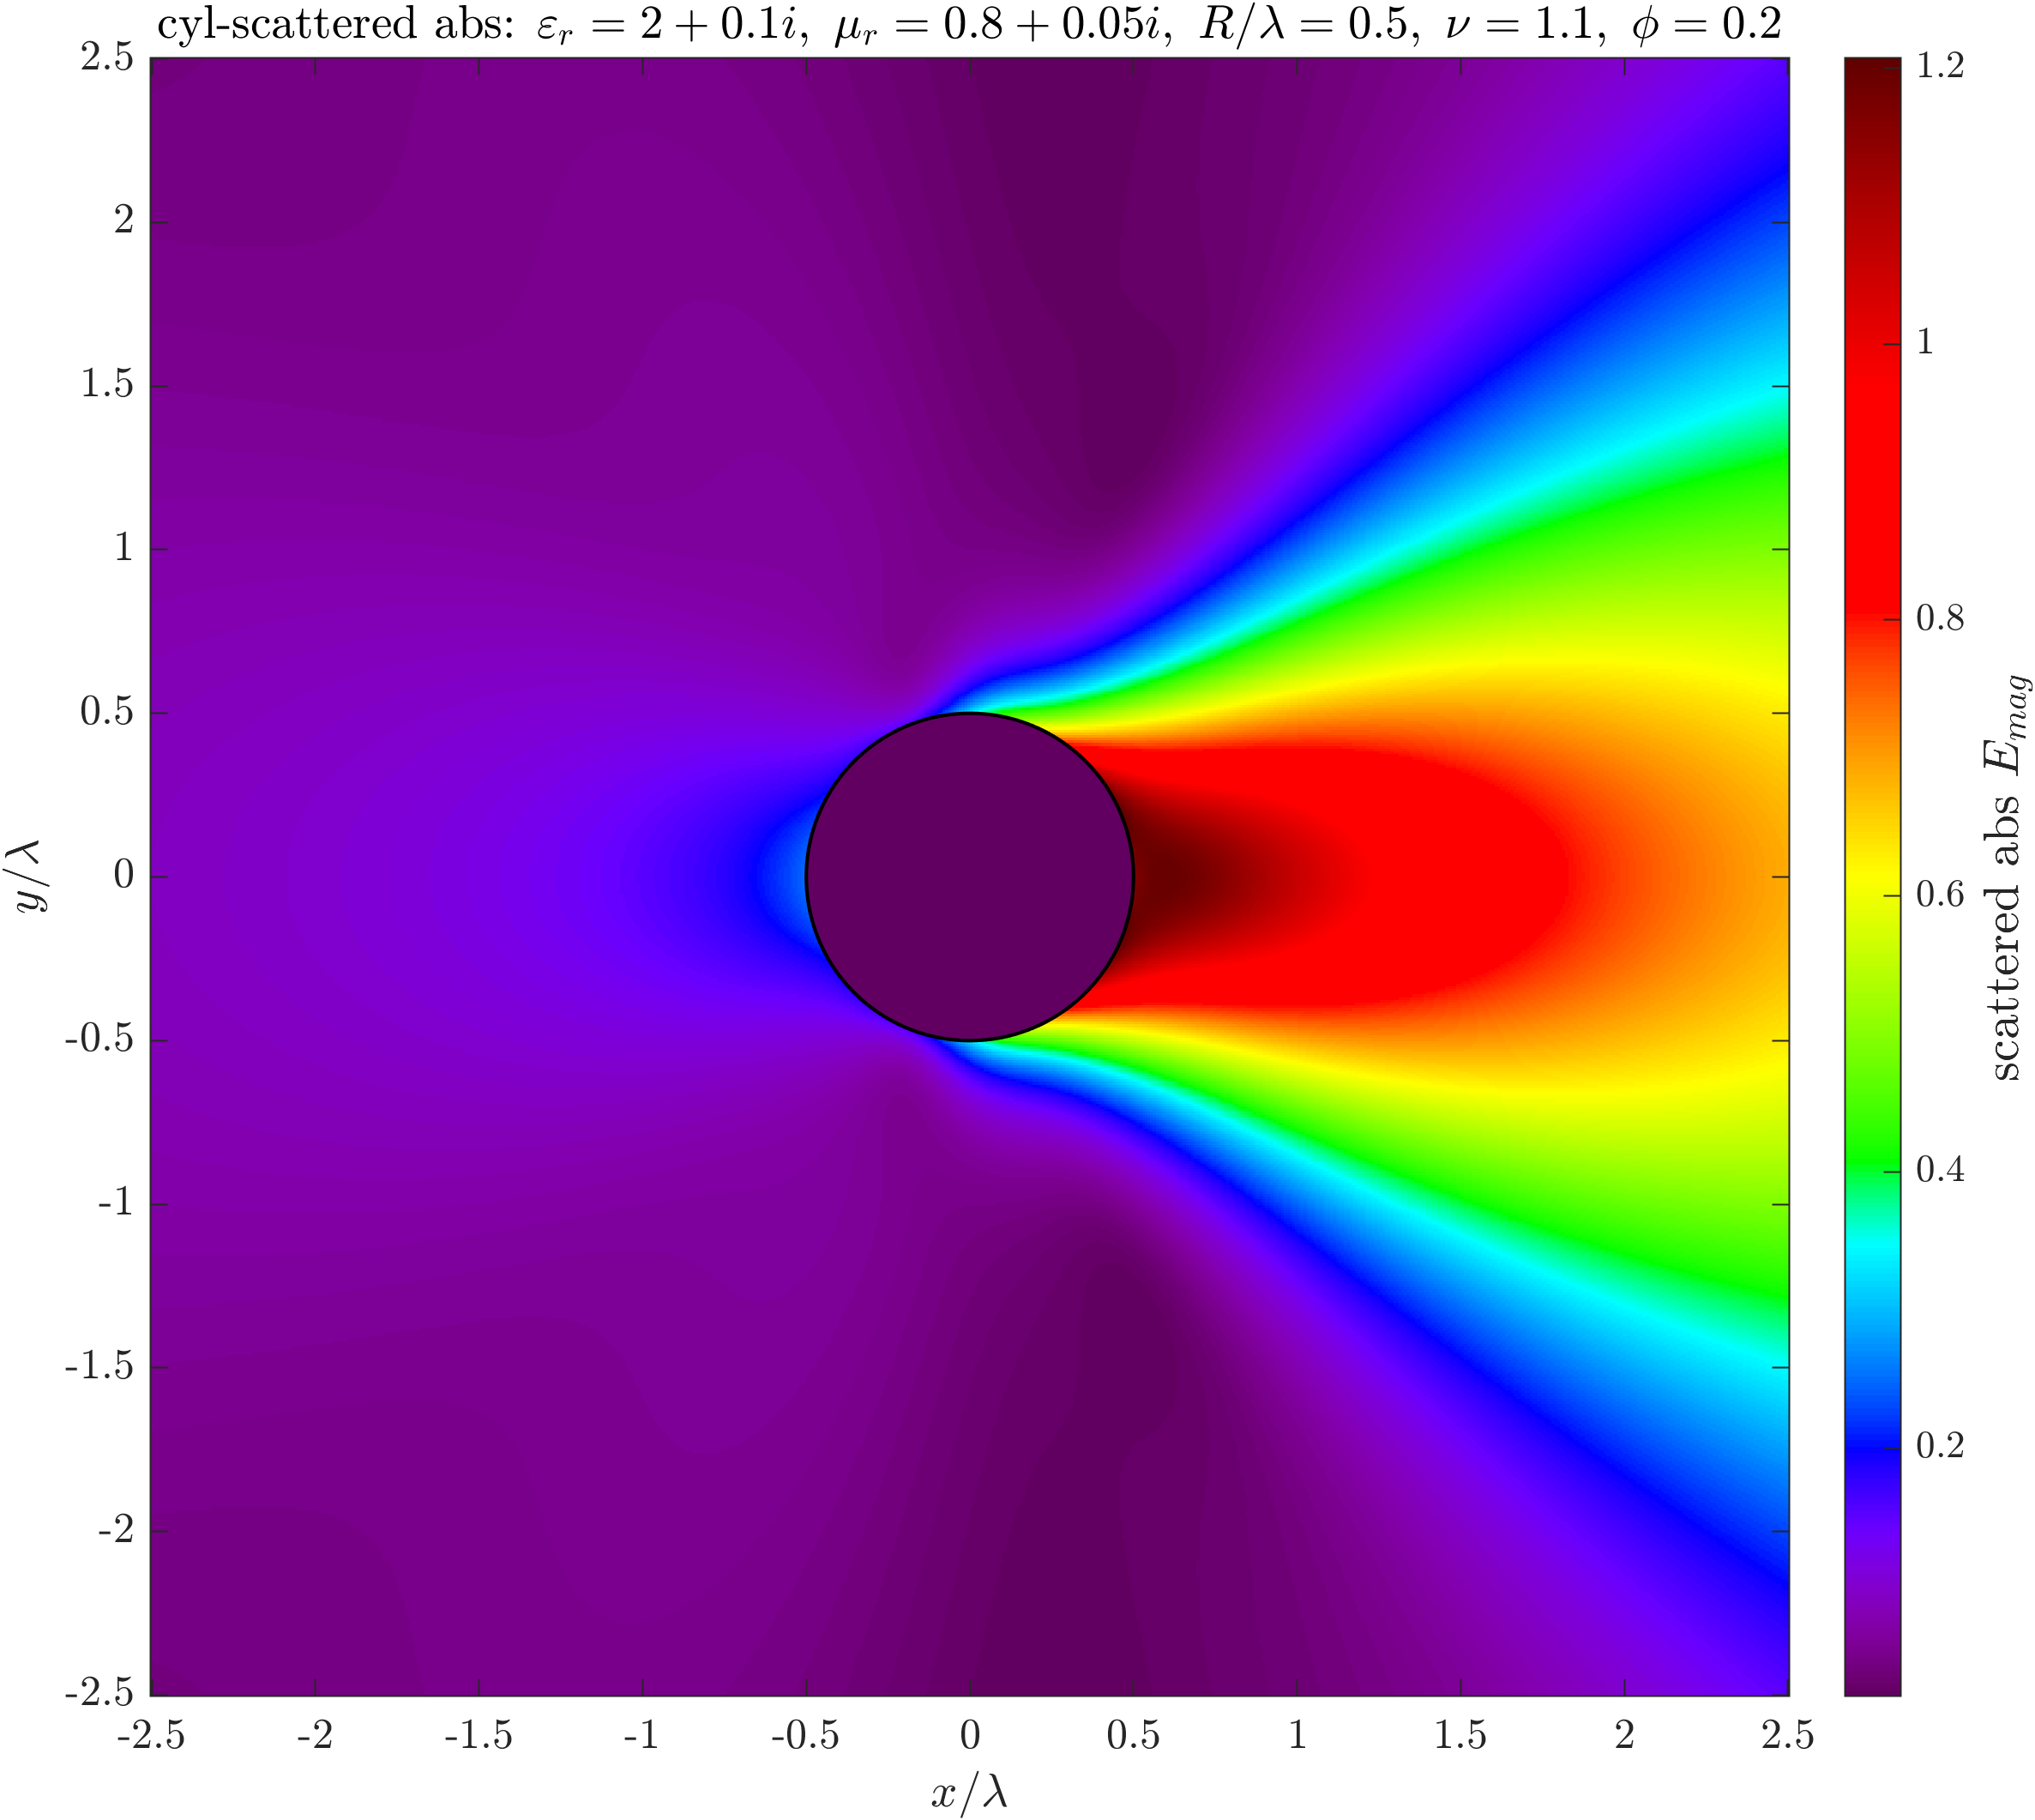
\includegraphics[width=\linewidth]{scattering_fig/lossy_small_cylinder_amplitude_magnitude.png}
			\caption{有损小柱，振幅大小}
			\label{柱体散射振幅比较图(对比有无损耗及不同半径)-有损小柱,振幅大小}
		\end{subfigure}

		\vspace{1em}

		% 第二行：有损大柱 (R/lambda=1.2, 有损耗)
		\begin{subfigure}{0.235\textwidth}
			\centering
			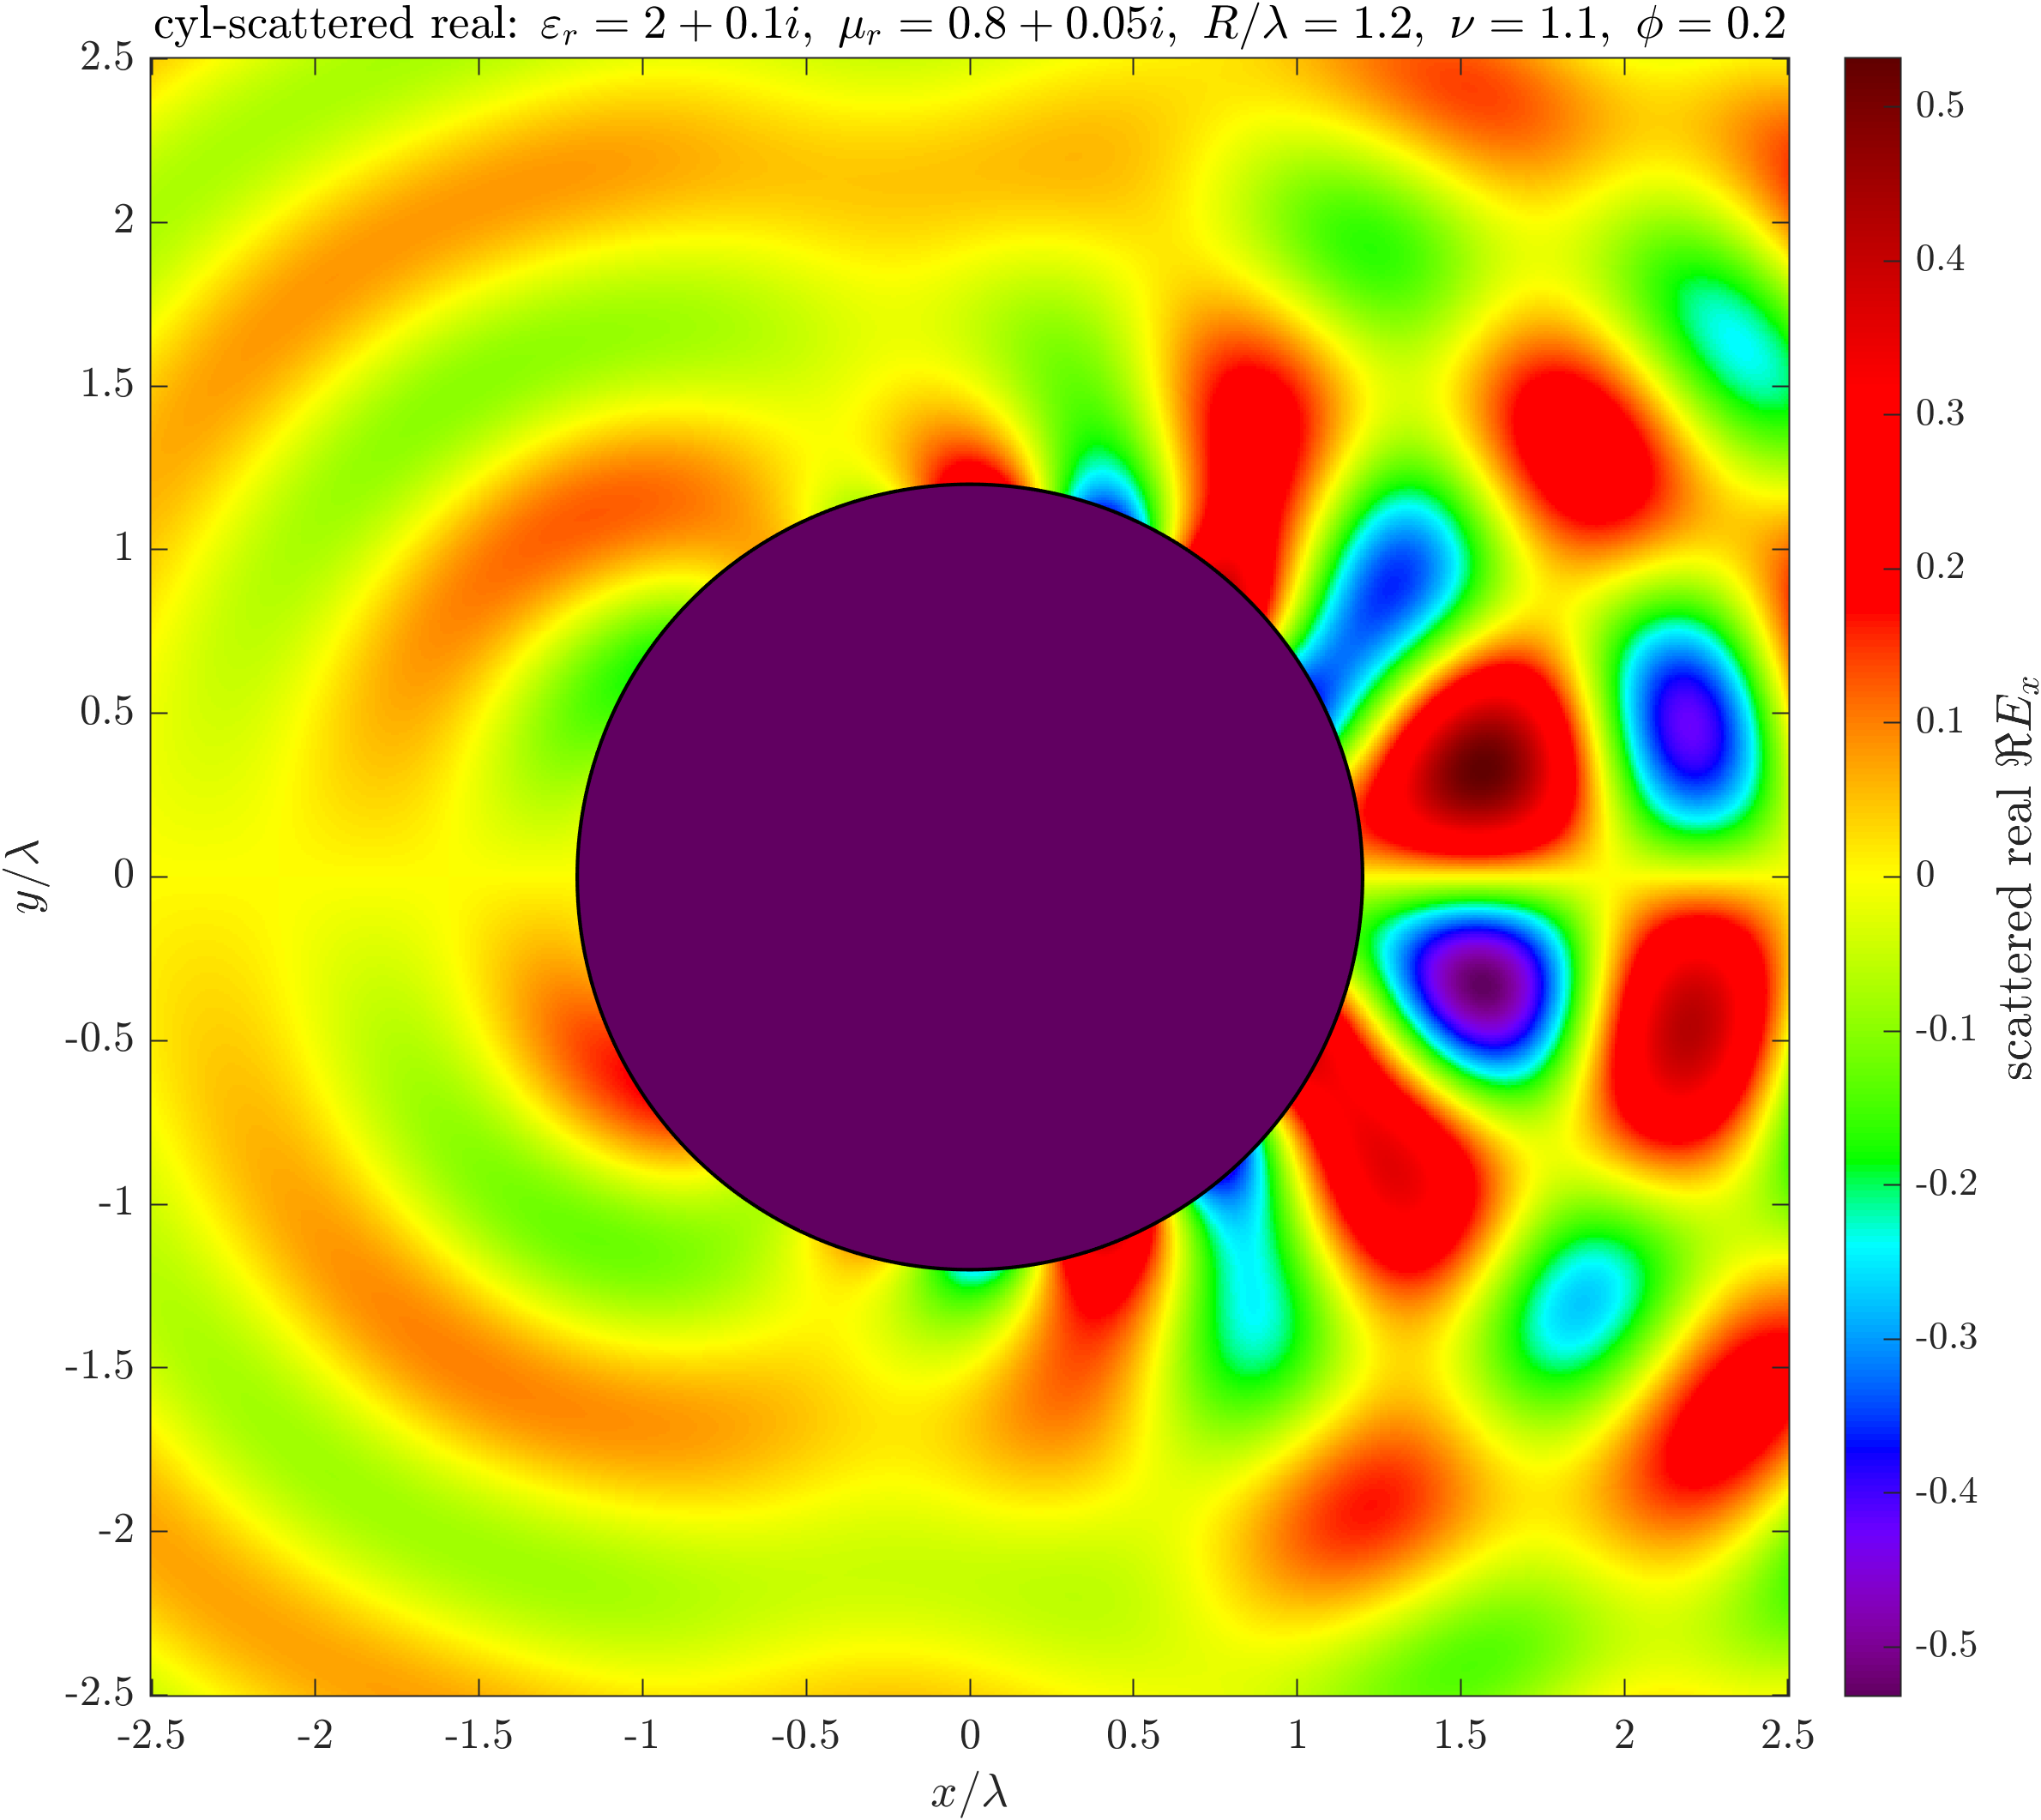
\includegraphics[width=\linewidth]{scattering_fig/lossy_large_cylinder_x_direction_real_part.png}
			\caption{有损大柱，\(x\)方向实部}
			\label{柱体散射振幅比较图(对比有无损耗及不同半径)-有损大柱,x方向实部}
		\end{subfigure}
		\hfill
		\begin{subfigure}{0.235\textwidth}
			\centering
			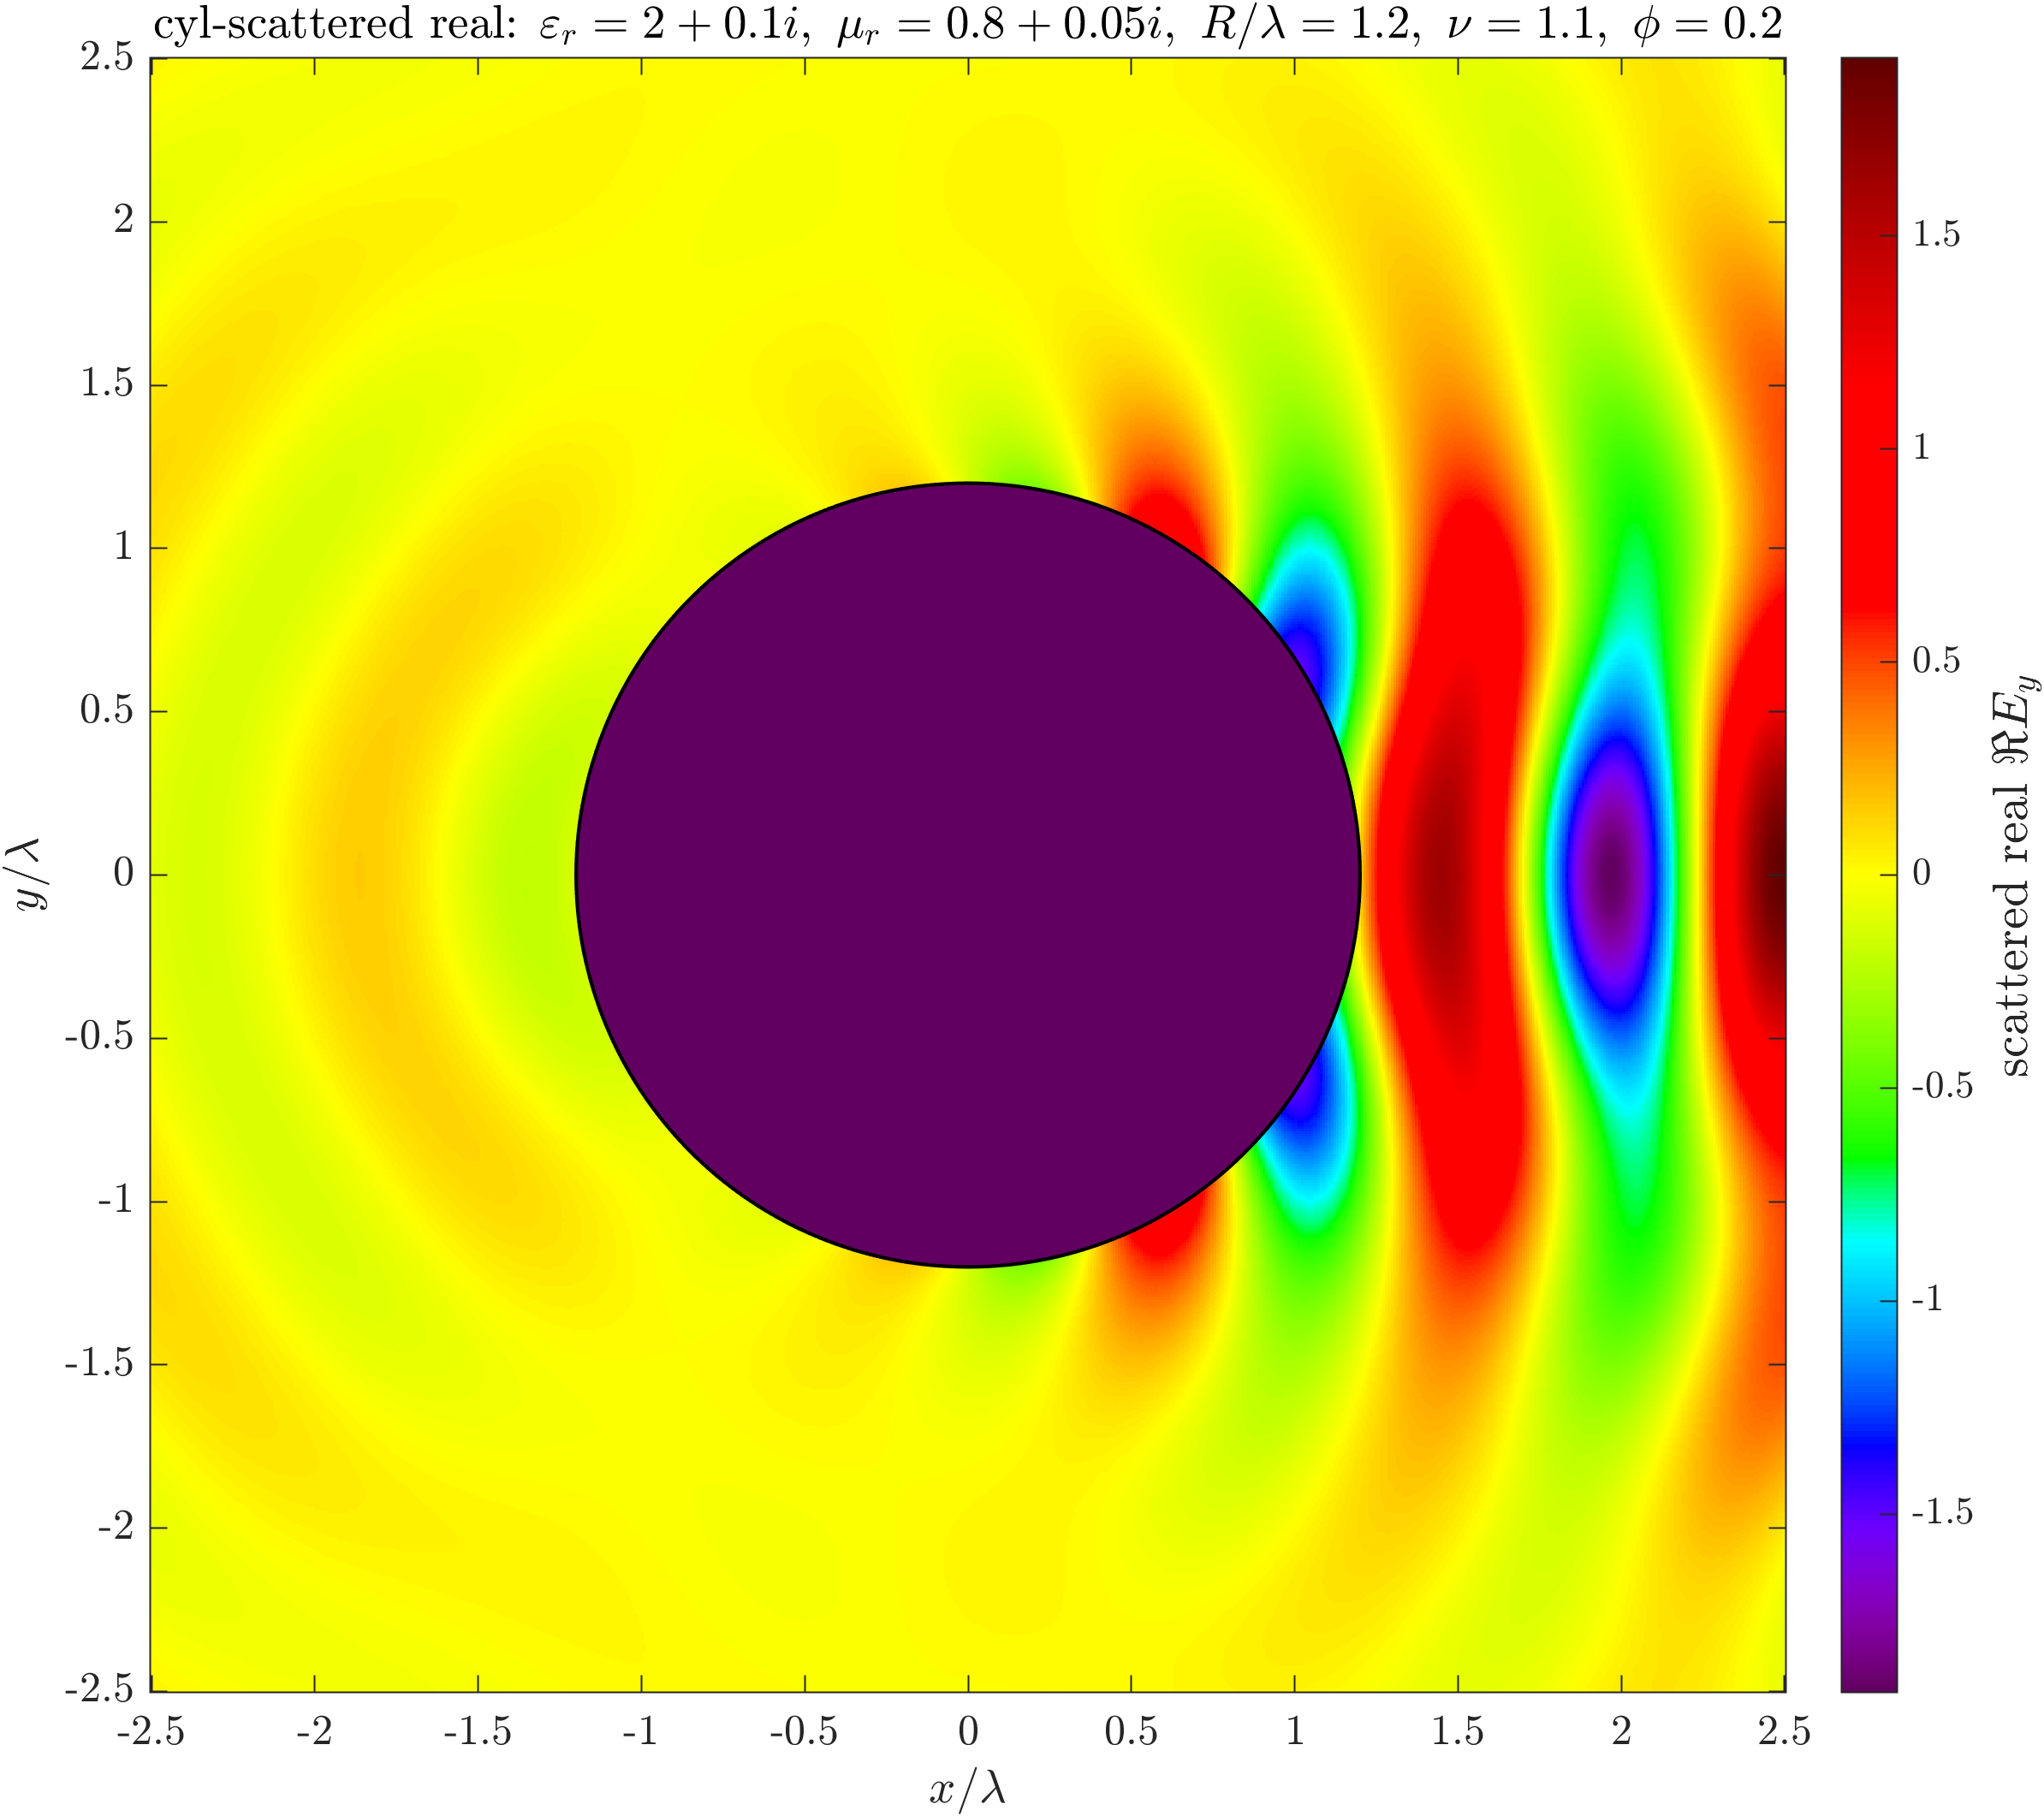
\includegraphics[width=\linewidth]{scattering_fig/lossy_large_cylinder_y_direction_real_part.png}
			\caption{有损大柱，\(y\)方向实部}
			\label{柱体散射振幅比较图(对比有无损耗及不同半径)-有损大柱,y方向实部}
		\end{subfigure}
		\hfill
		\begin{subfigure}{0.235\textwidth}
			\centering
			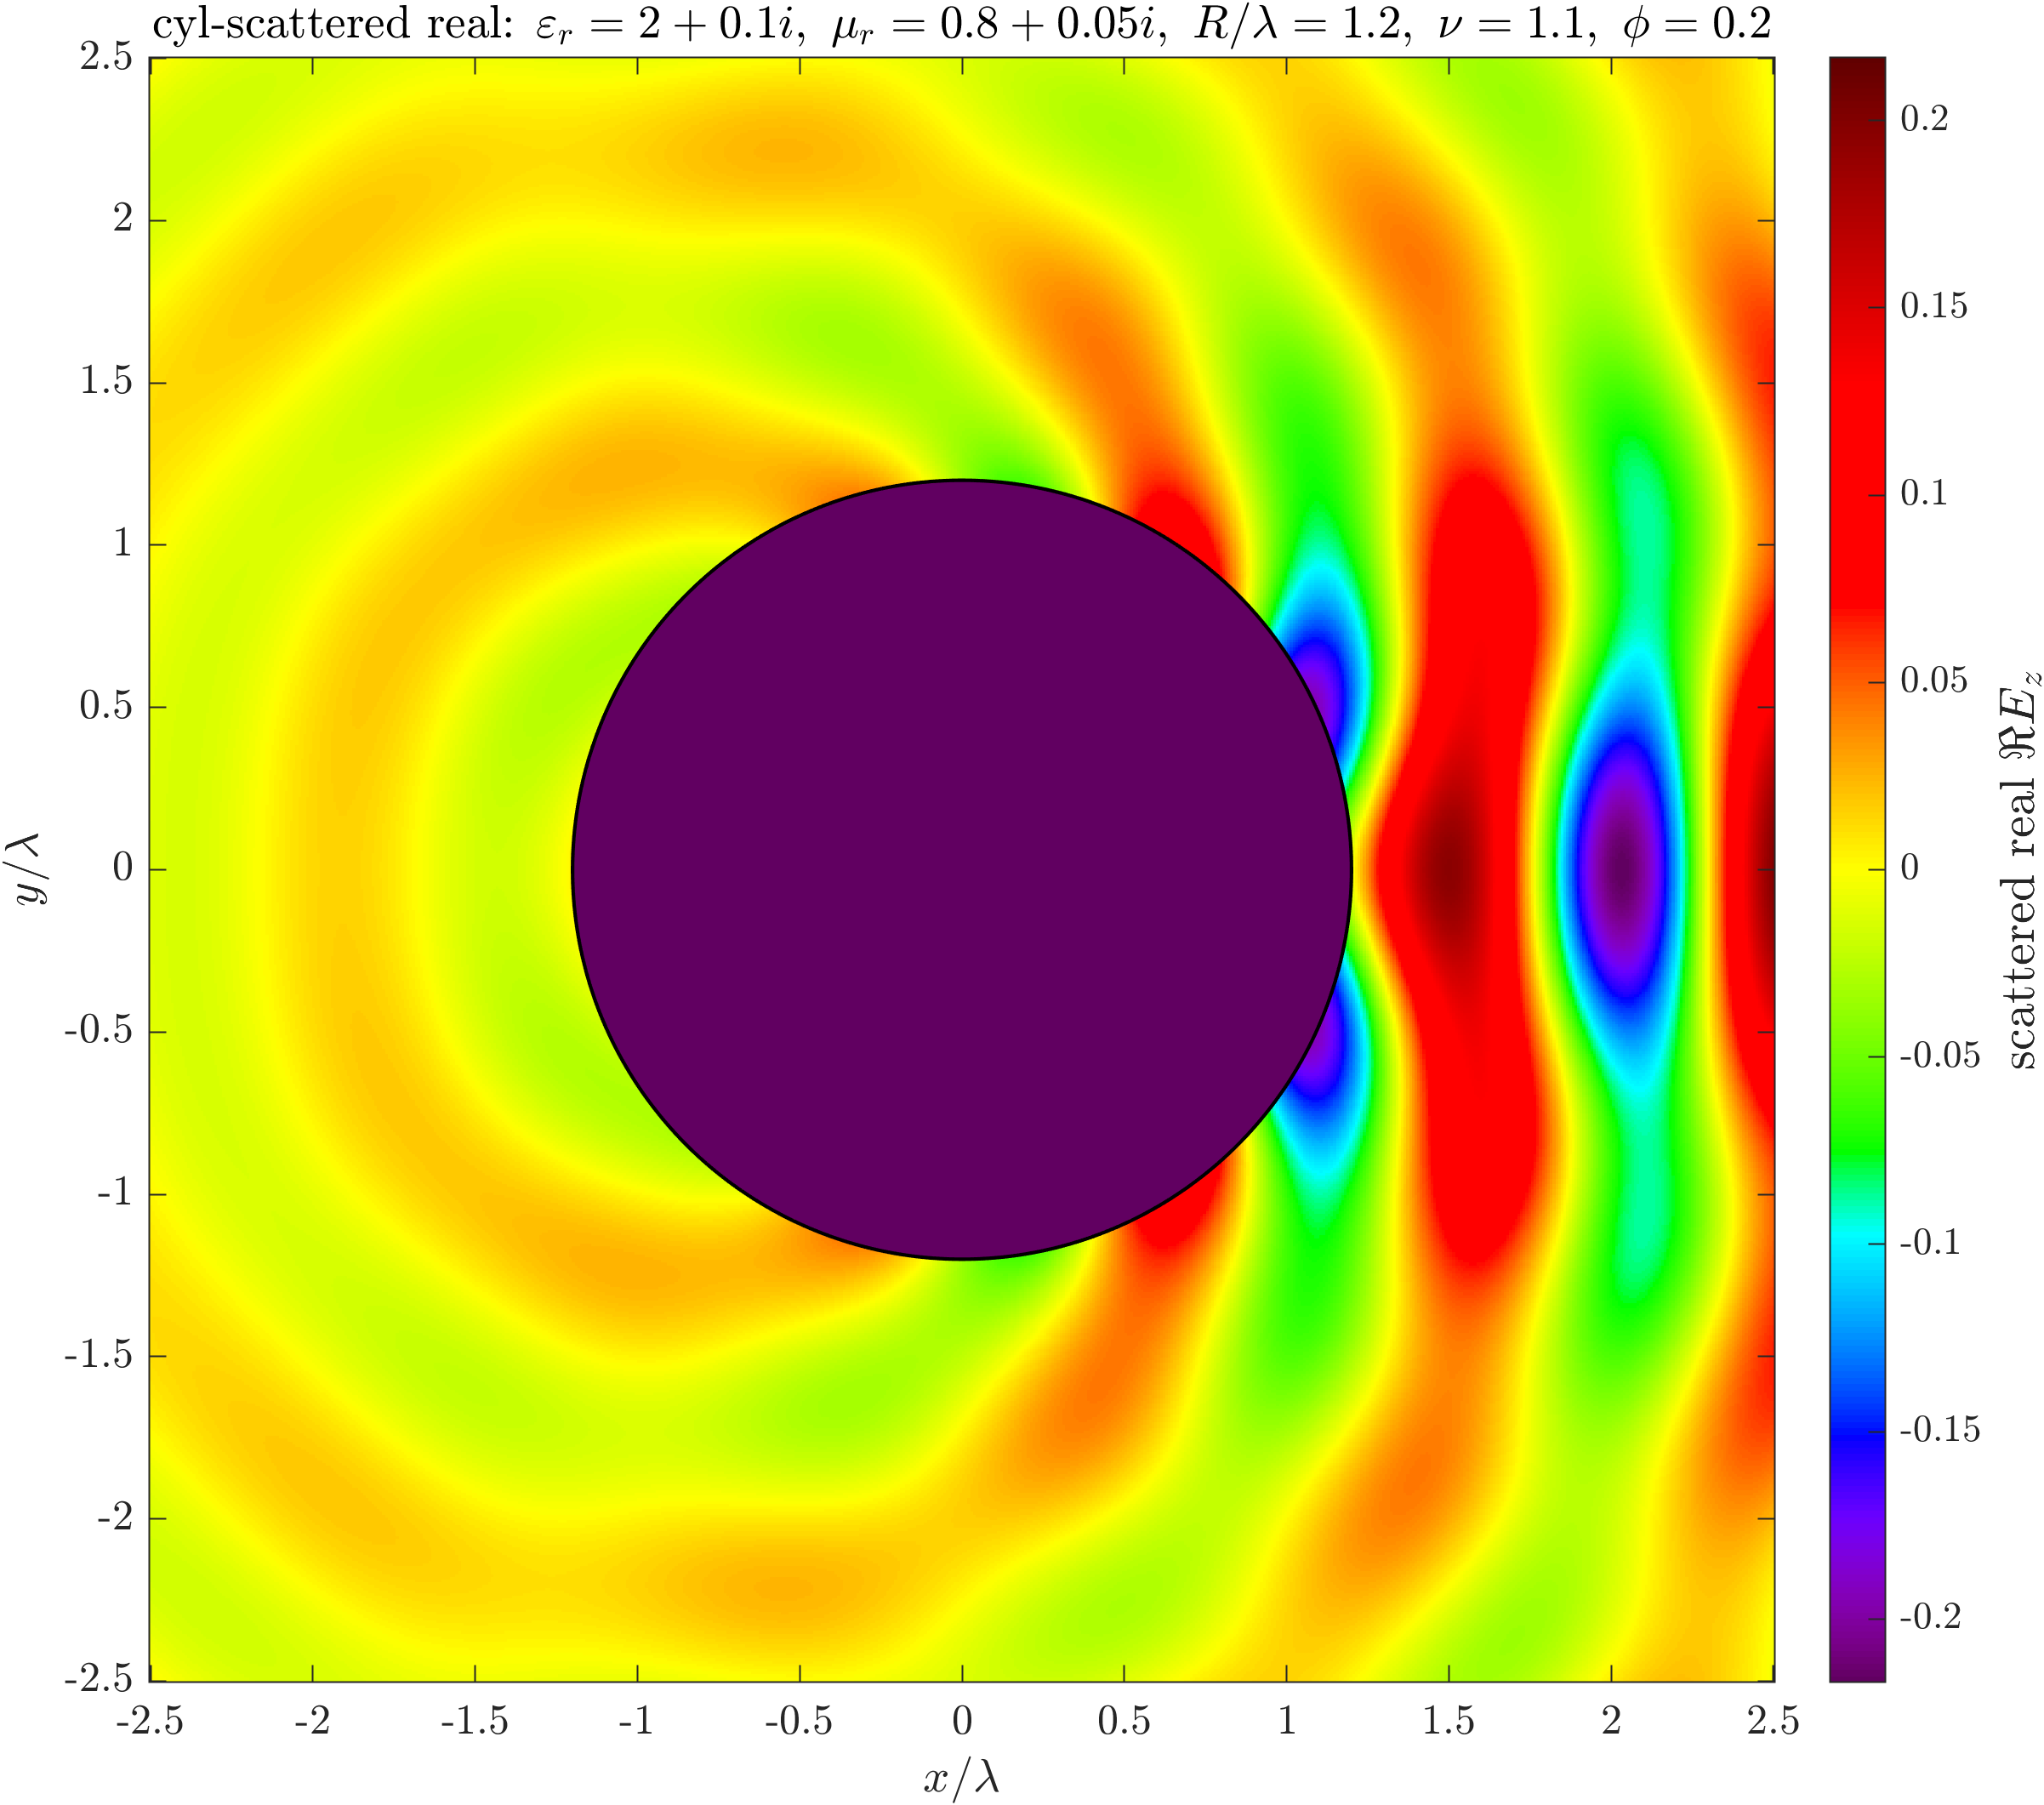
\includegraphics[width=\linewidth]{scattering_fig/lossy_large_cylinder_z_direction_real_part.png}
			\caption{有损大柱，\(z\)方向实部}
			\label{柱体散射振幅比较图(对比有无损耗及不同半径)-有损大柱,z方向实部}
		\end{subfigure}
		\hfill
		\begin{subfigure}{0.235\textwidth}
			\centering
			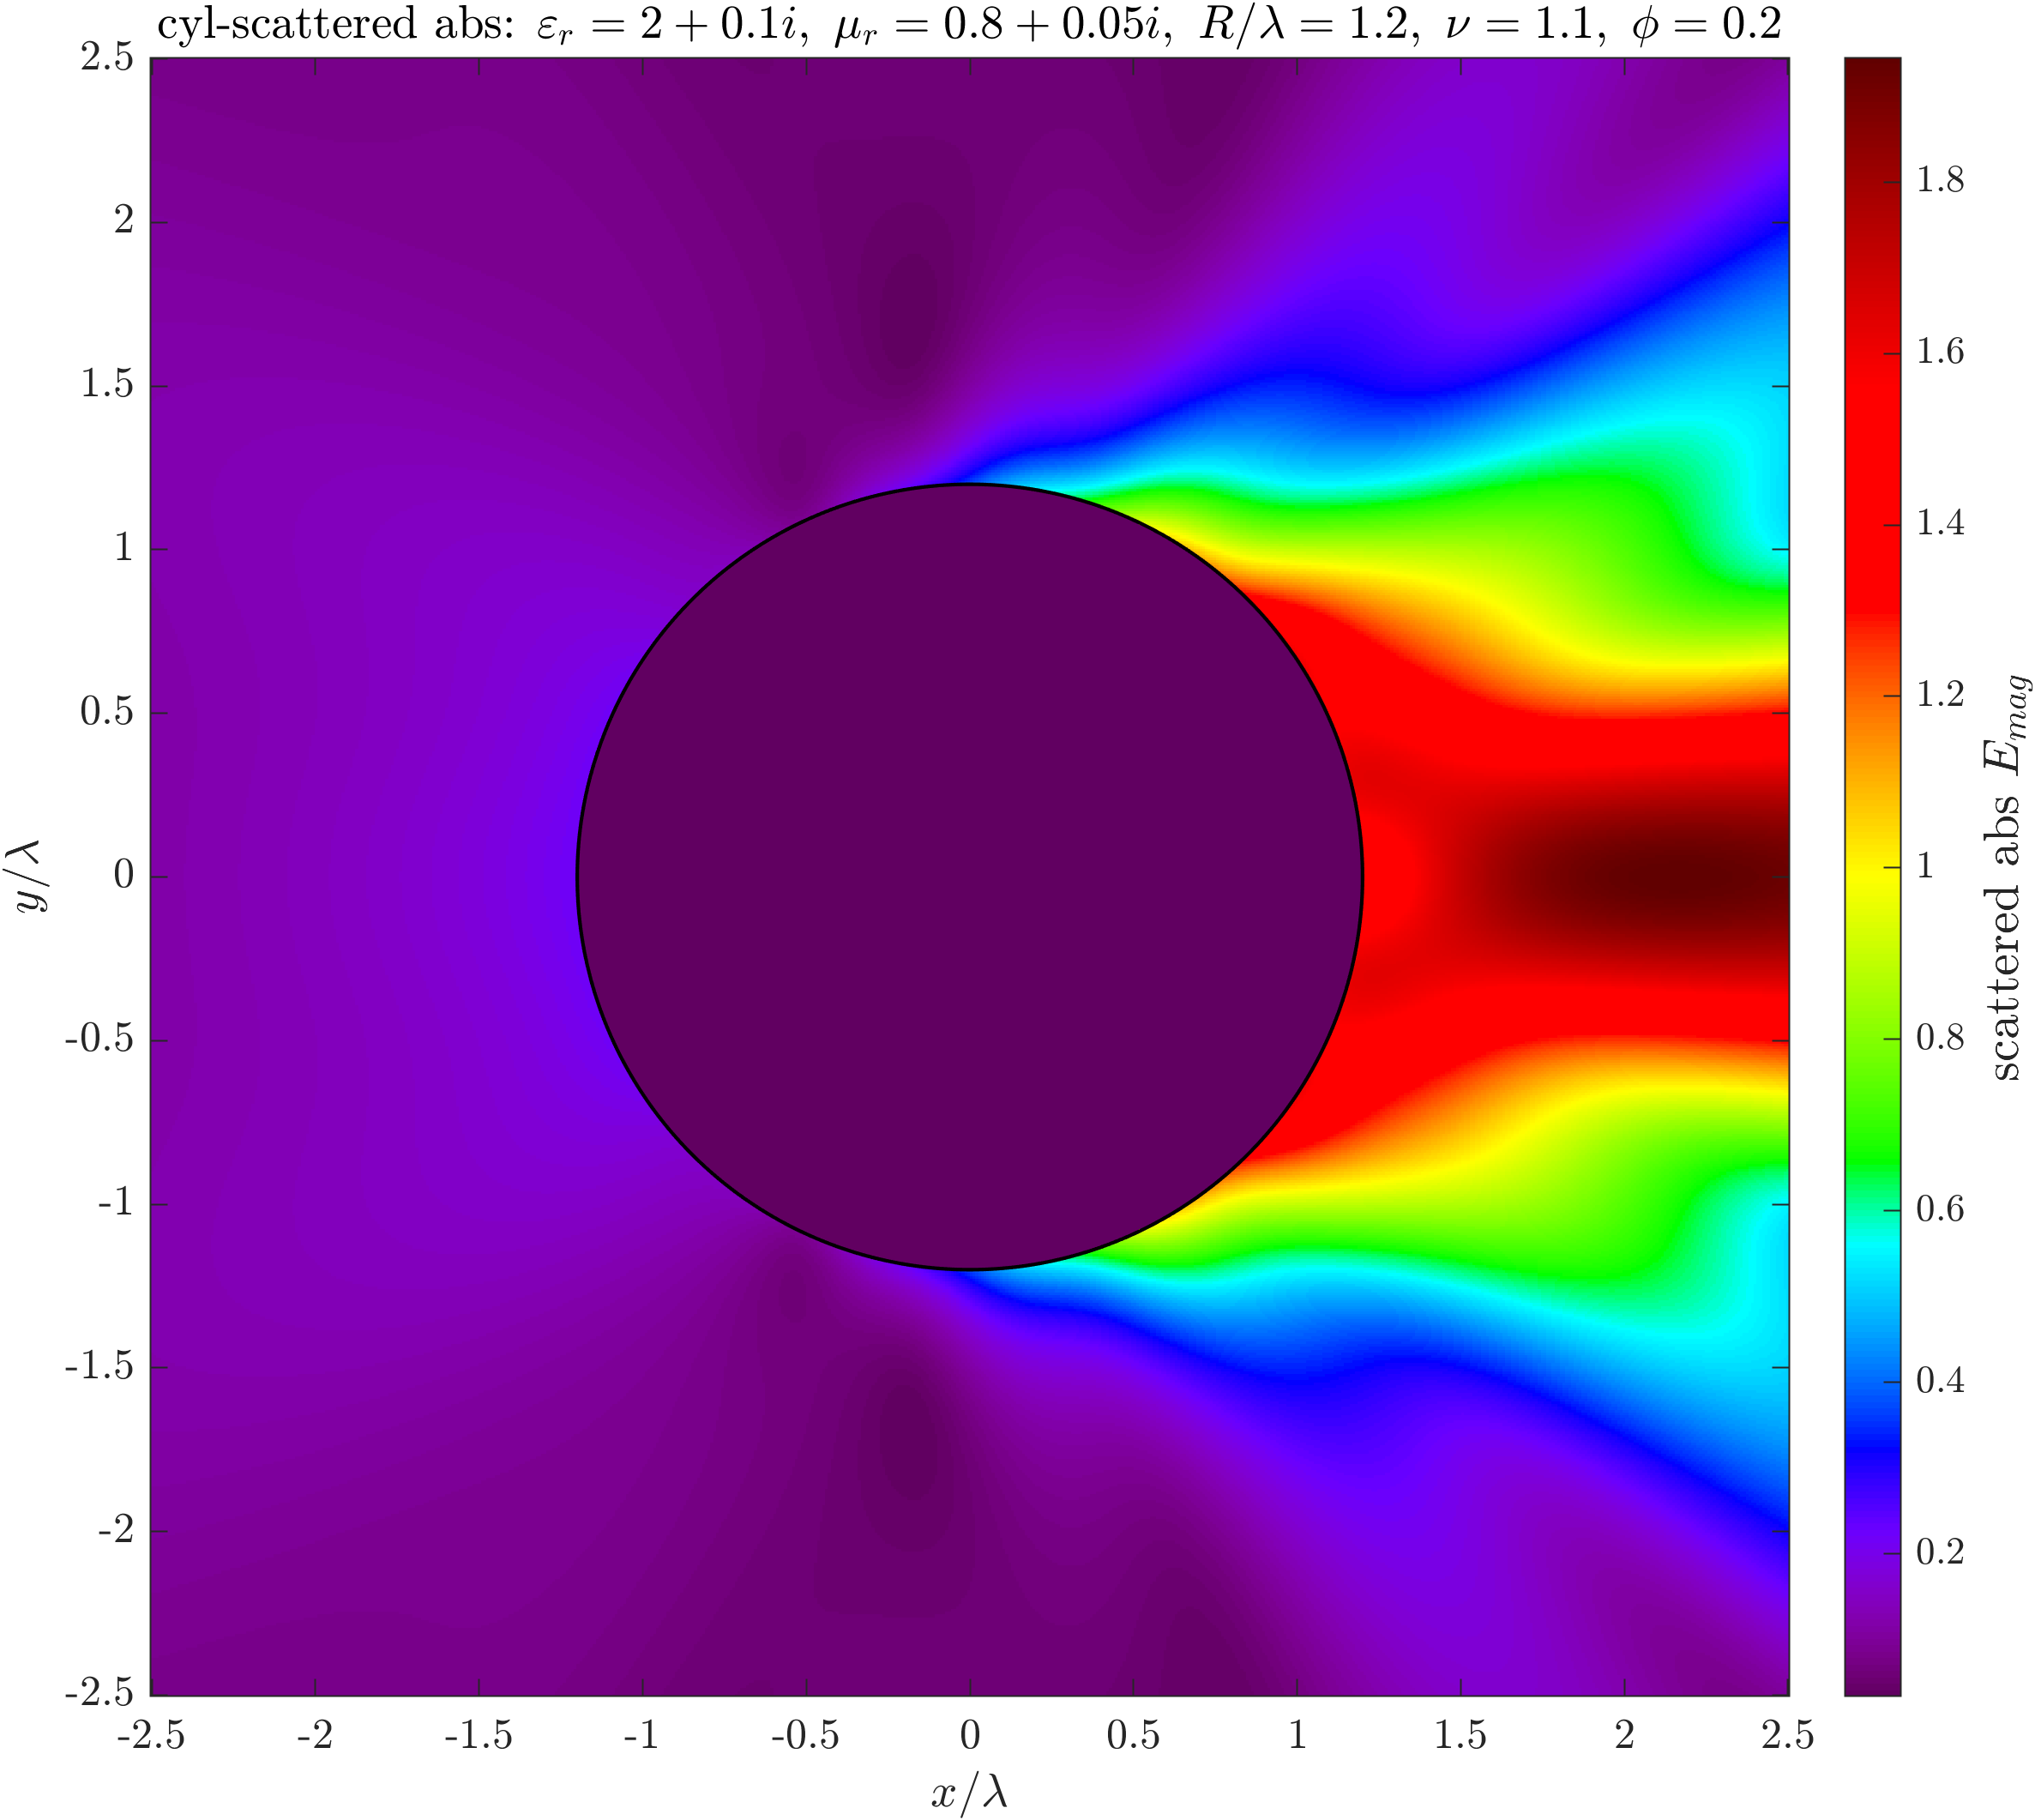
\includegraphics[width=\linewidth]{scattering_fig/lossy_large_cylinder_amplitude_magnitude.png}
			\caption{有损大柱，振幅大小}
			\label{柱体散射振幅比较图(对比有无损耗及不同半径)-有损大柱,振幅大小}
		\end{subfigure}

		\vspace{1em}

		% 第三行：无损大柱 (R/lambda=1.2, 无损耗)
		\begin{subfigure}{0.235\textwidth}
			\centering
			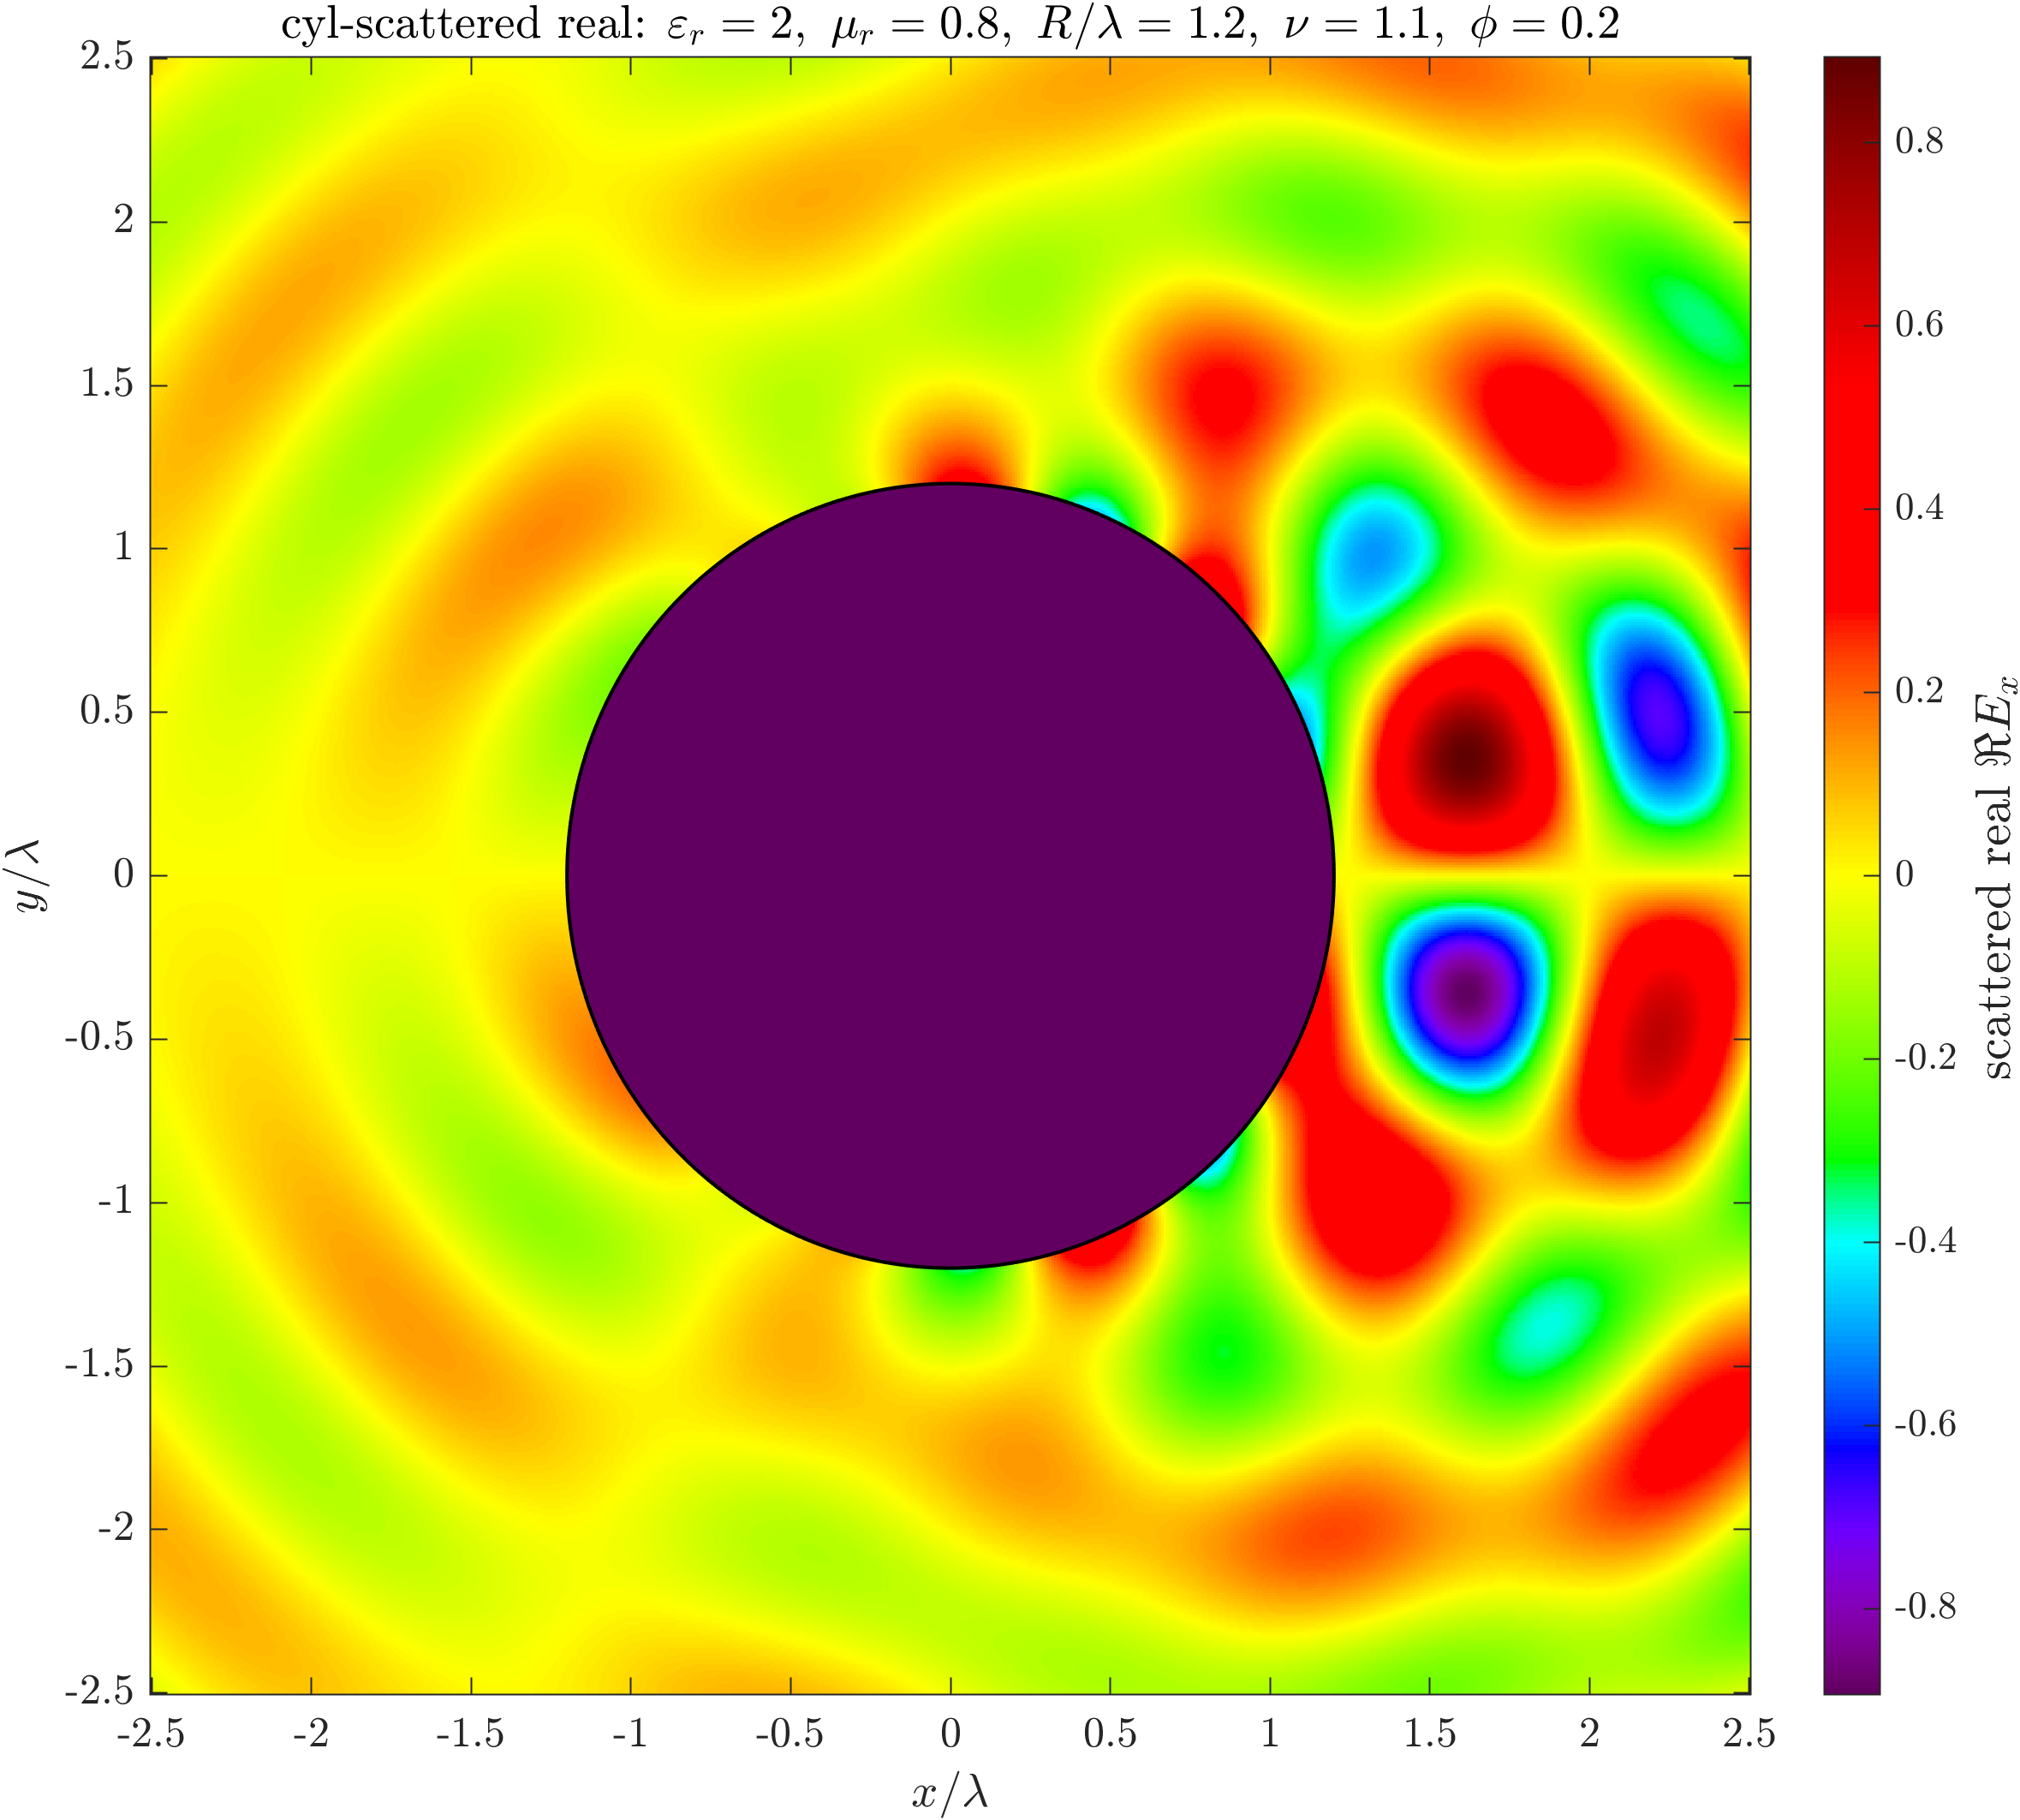
\includegraphics[width=\linewidth]{scattering_fig/lossless_large_cylinder_x_direction_real_part.png}
			\caption{无损大柱，\(x\)方向实部}
			\label{柱体散射振幅比较图(对比有无损耗及不同半径)-无损大柱,x方向实部}
		\end{subfigure}
		\hfill
		\begin{subfigure}{0.235\textwidth}
			\centering
			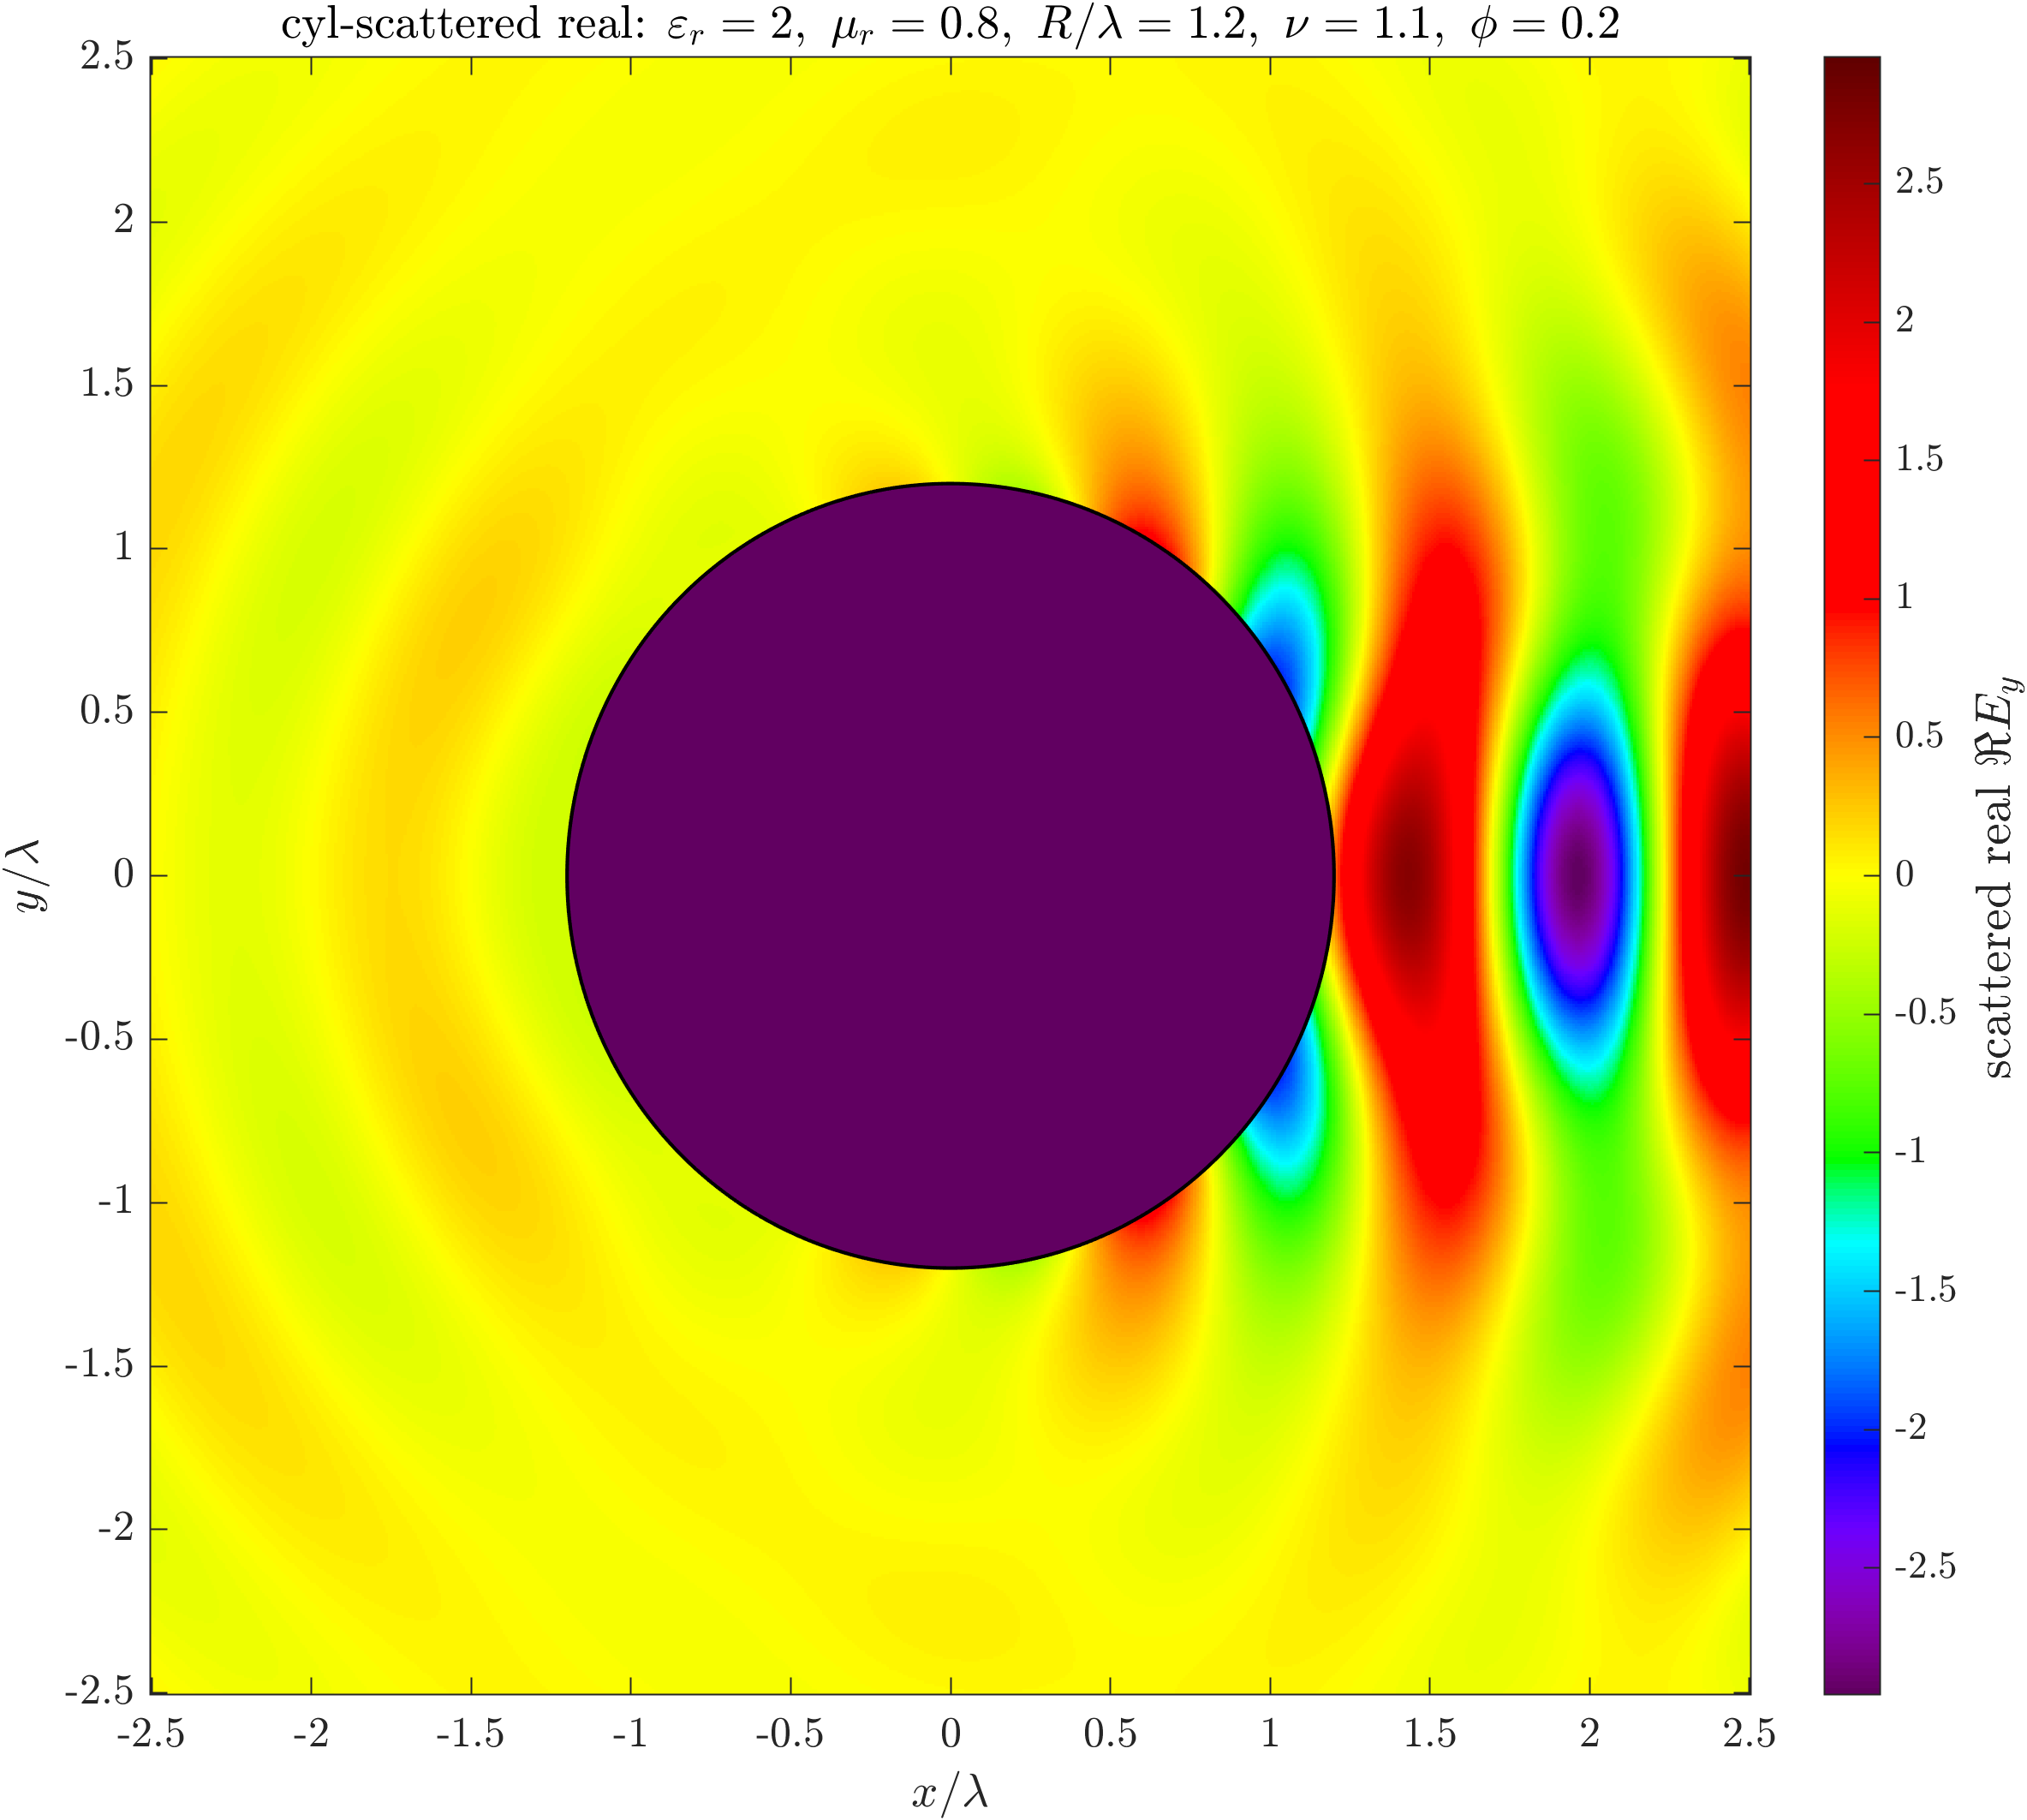
\includegraphics[width=\linewidth]{scattering_fig/lossless_large_cylinder_y_direction_real_part.png}
			\caption{无损大柱，\(y\)方向实部}
			\label{柱体散射振幅比较图(对比有无损耗及不同半径)-无损大柱,y方向实部}
		\end{subfigure}
		\hfill
		\begin{subfigure}{0.235\textwidth}
			\centering
			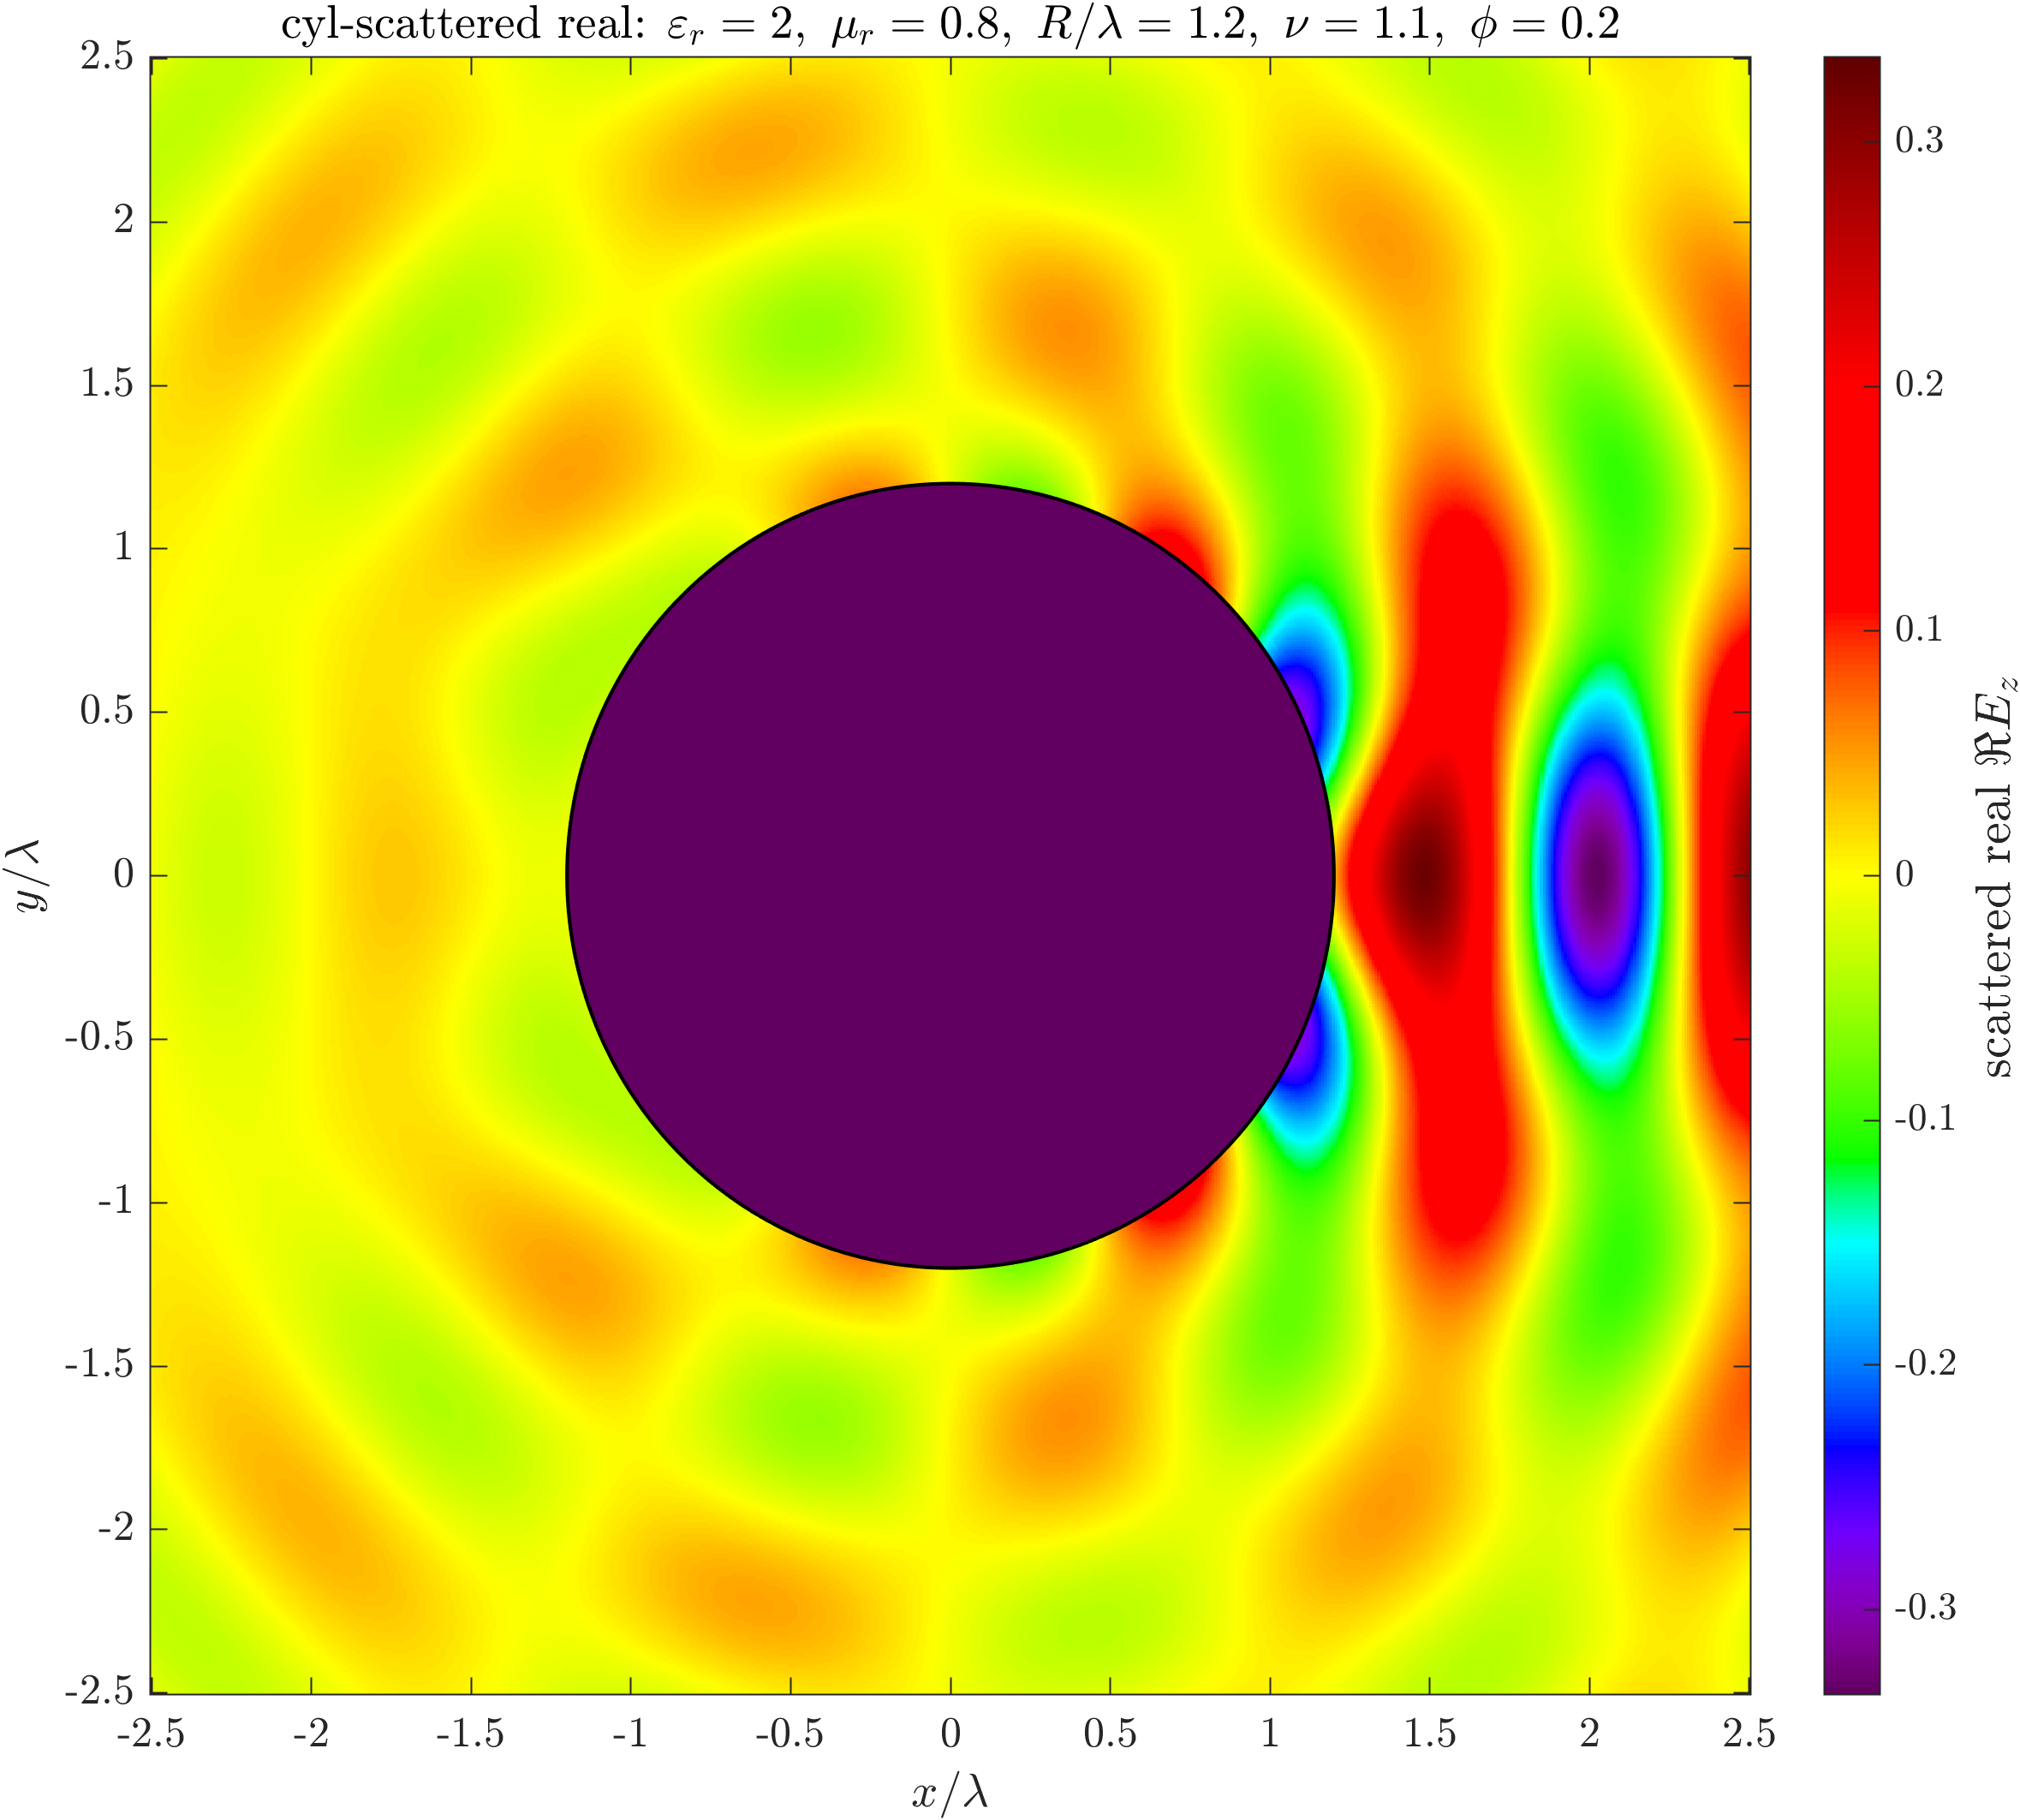
\includegraphics[width=\linewidth]{scattering_fig/lossless_large_cylinder_z_direction_real_part.png}
			\caption{无损大柱，\(z\)方向实部}
			\label{柱体散射振幅比较图(对比有无损耗及不同半径)-无损大柱,z方向实部}
		\end{subfigure}
		\hfill
		\begin{subfigure}{0.235\textwidth}
			\centering
			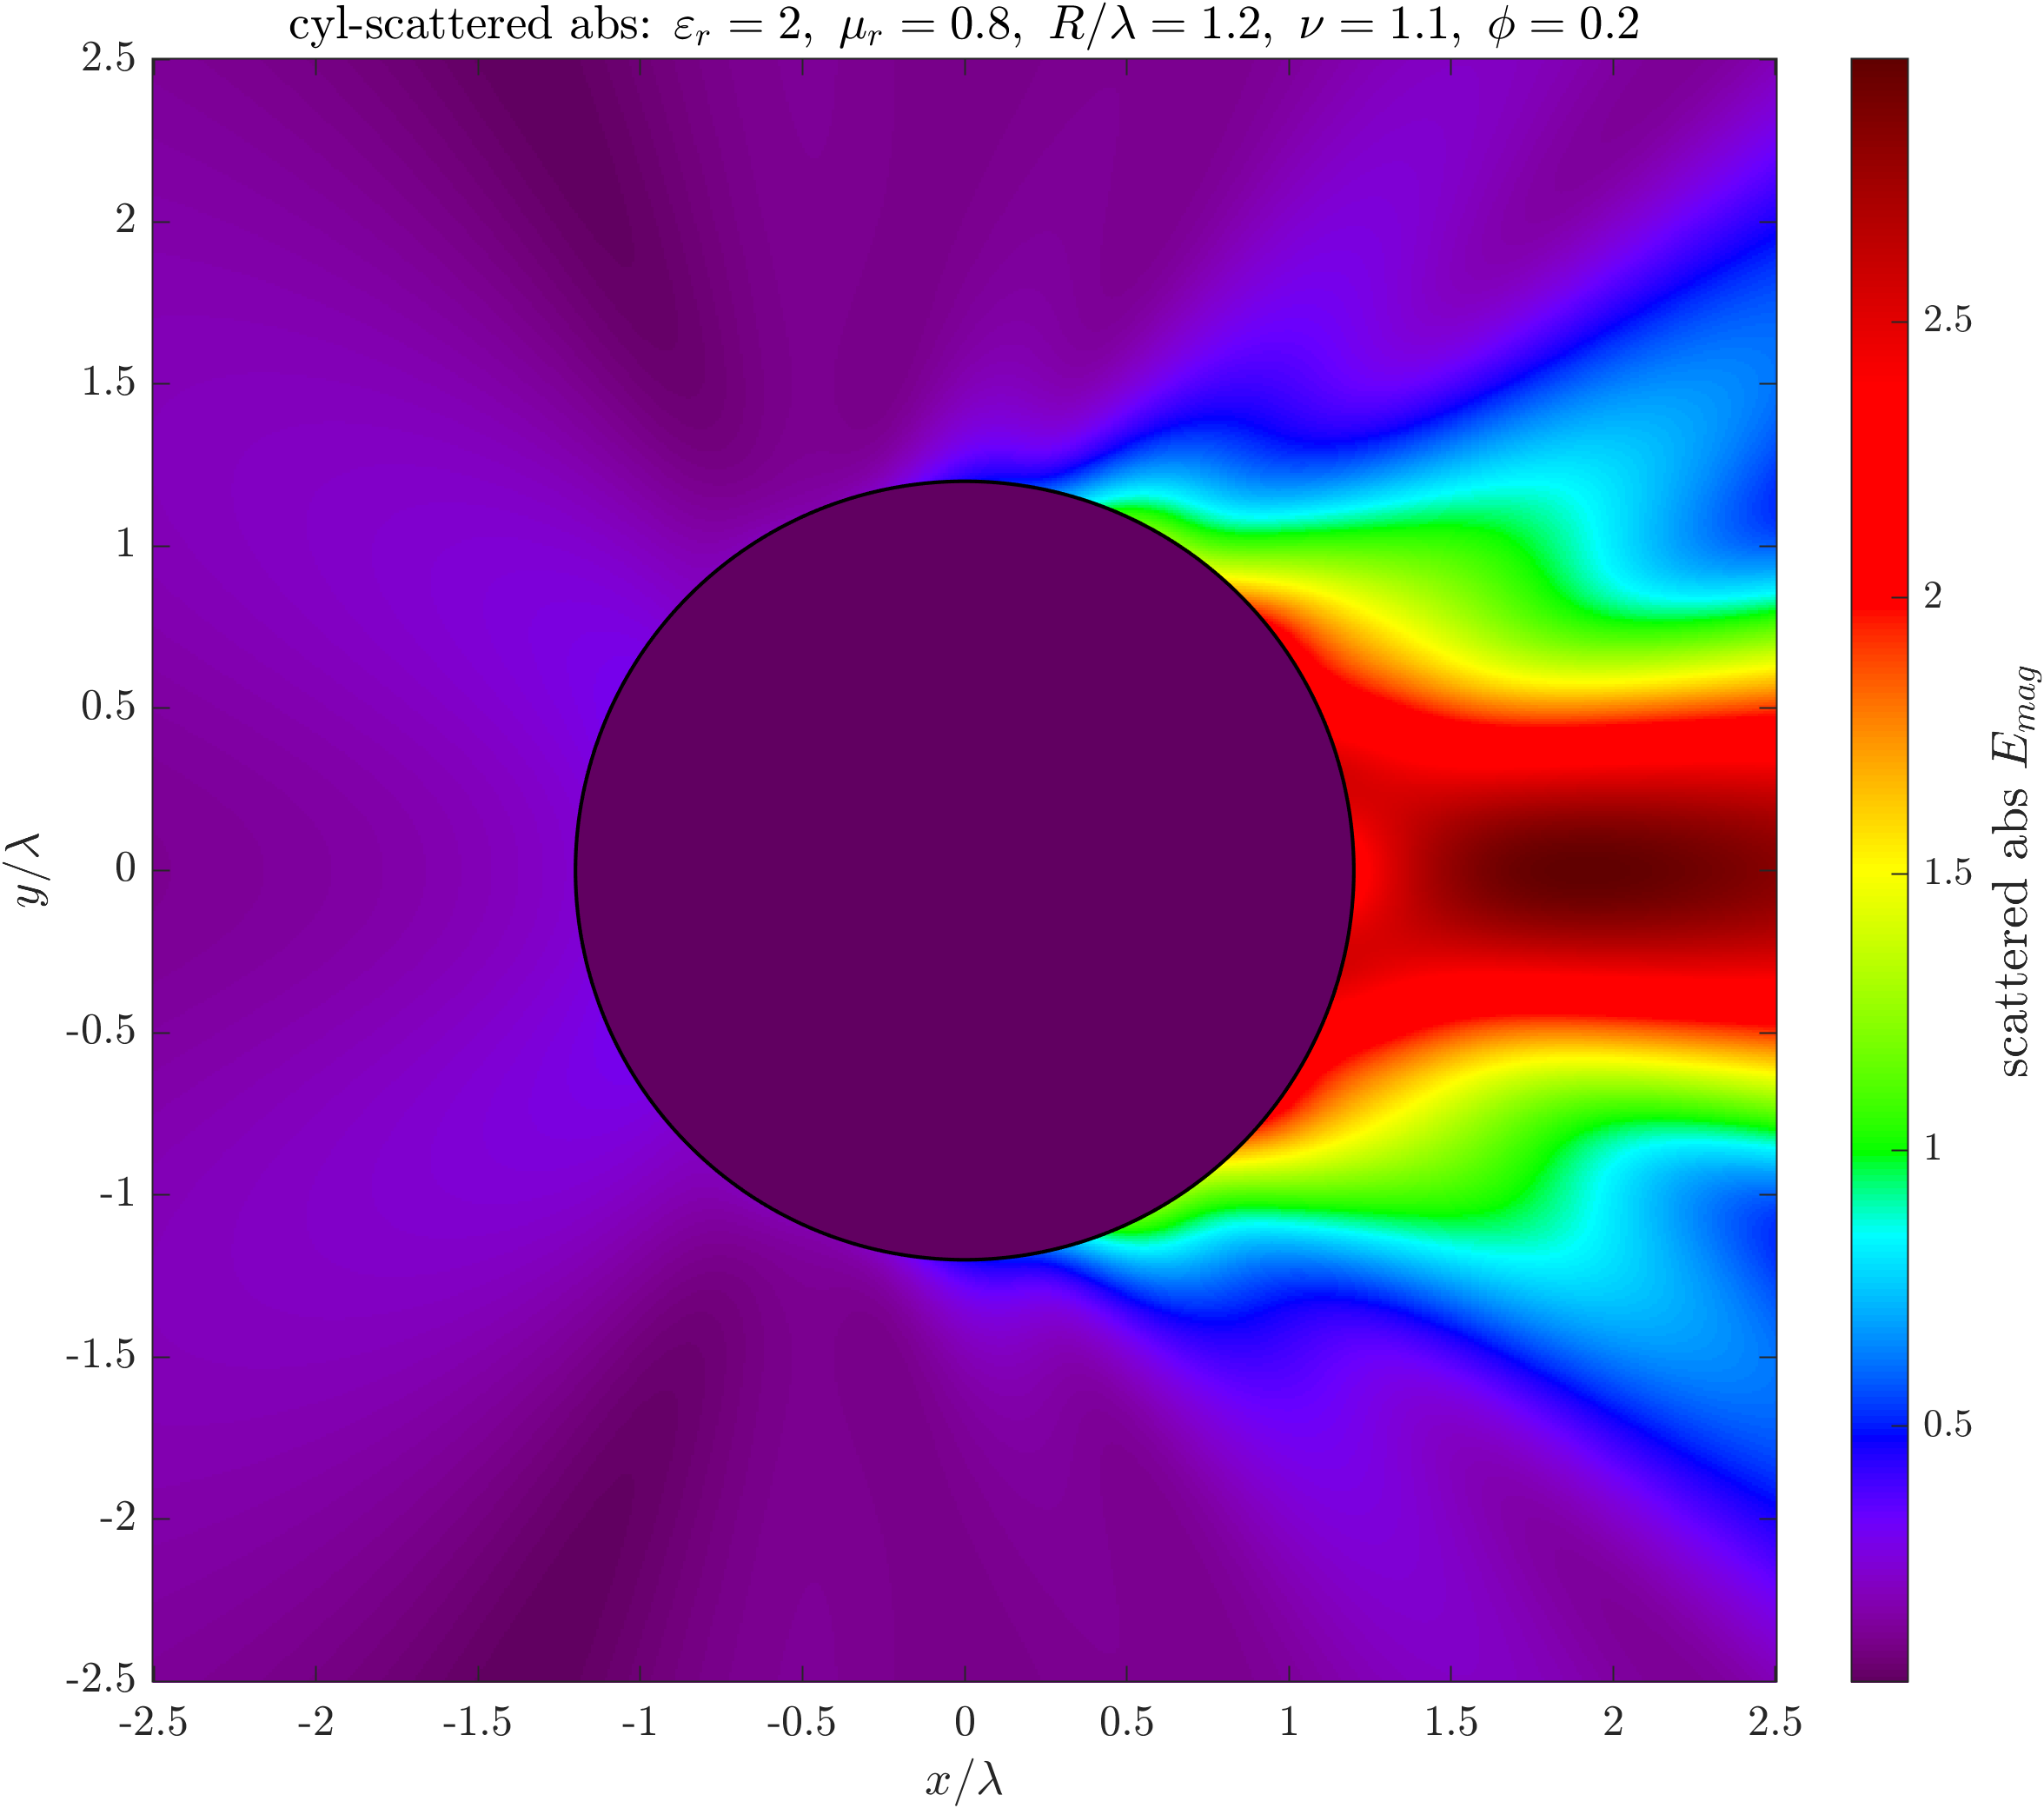
\includegraphics[width=\linewidth]{scattering_fig/lossless_large_cylinder_amplitude_magnitude.png}
			\caption{无损大柱，振幅大小}
			\label{柱体散射振幅比较图(对比有无损耗及不同半径)-无损大柱,振幅大小}
		\end{subfigure}

		\caption{柱体散射振幅比较图（对比有无损耗及不同半径）}
		\label{柱体散射振幅比较图(对比有无损耗及不同半径)}
		\label{fig:cylinder-scattering-comparison-loss}
	\end{figure}

	% 柱体总场振幅比较图（一行，三个图）
	\begin{figure}[H]
		\centering
		% 第一个：有损小柱总场振幅
		\begin{subfigure}{0.3\textwidth}
			\centering
			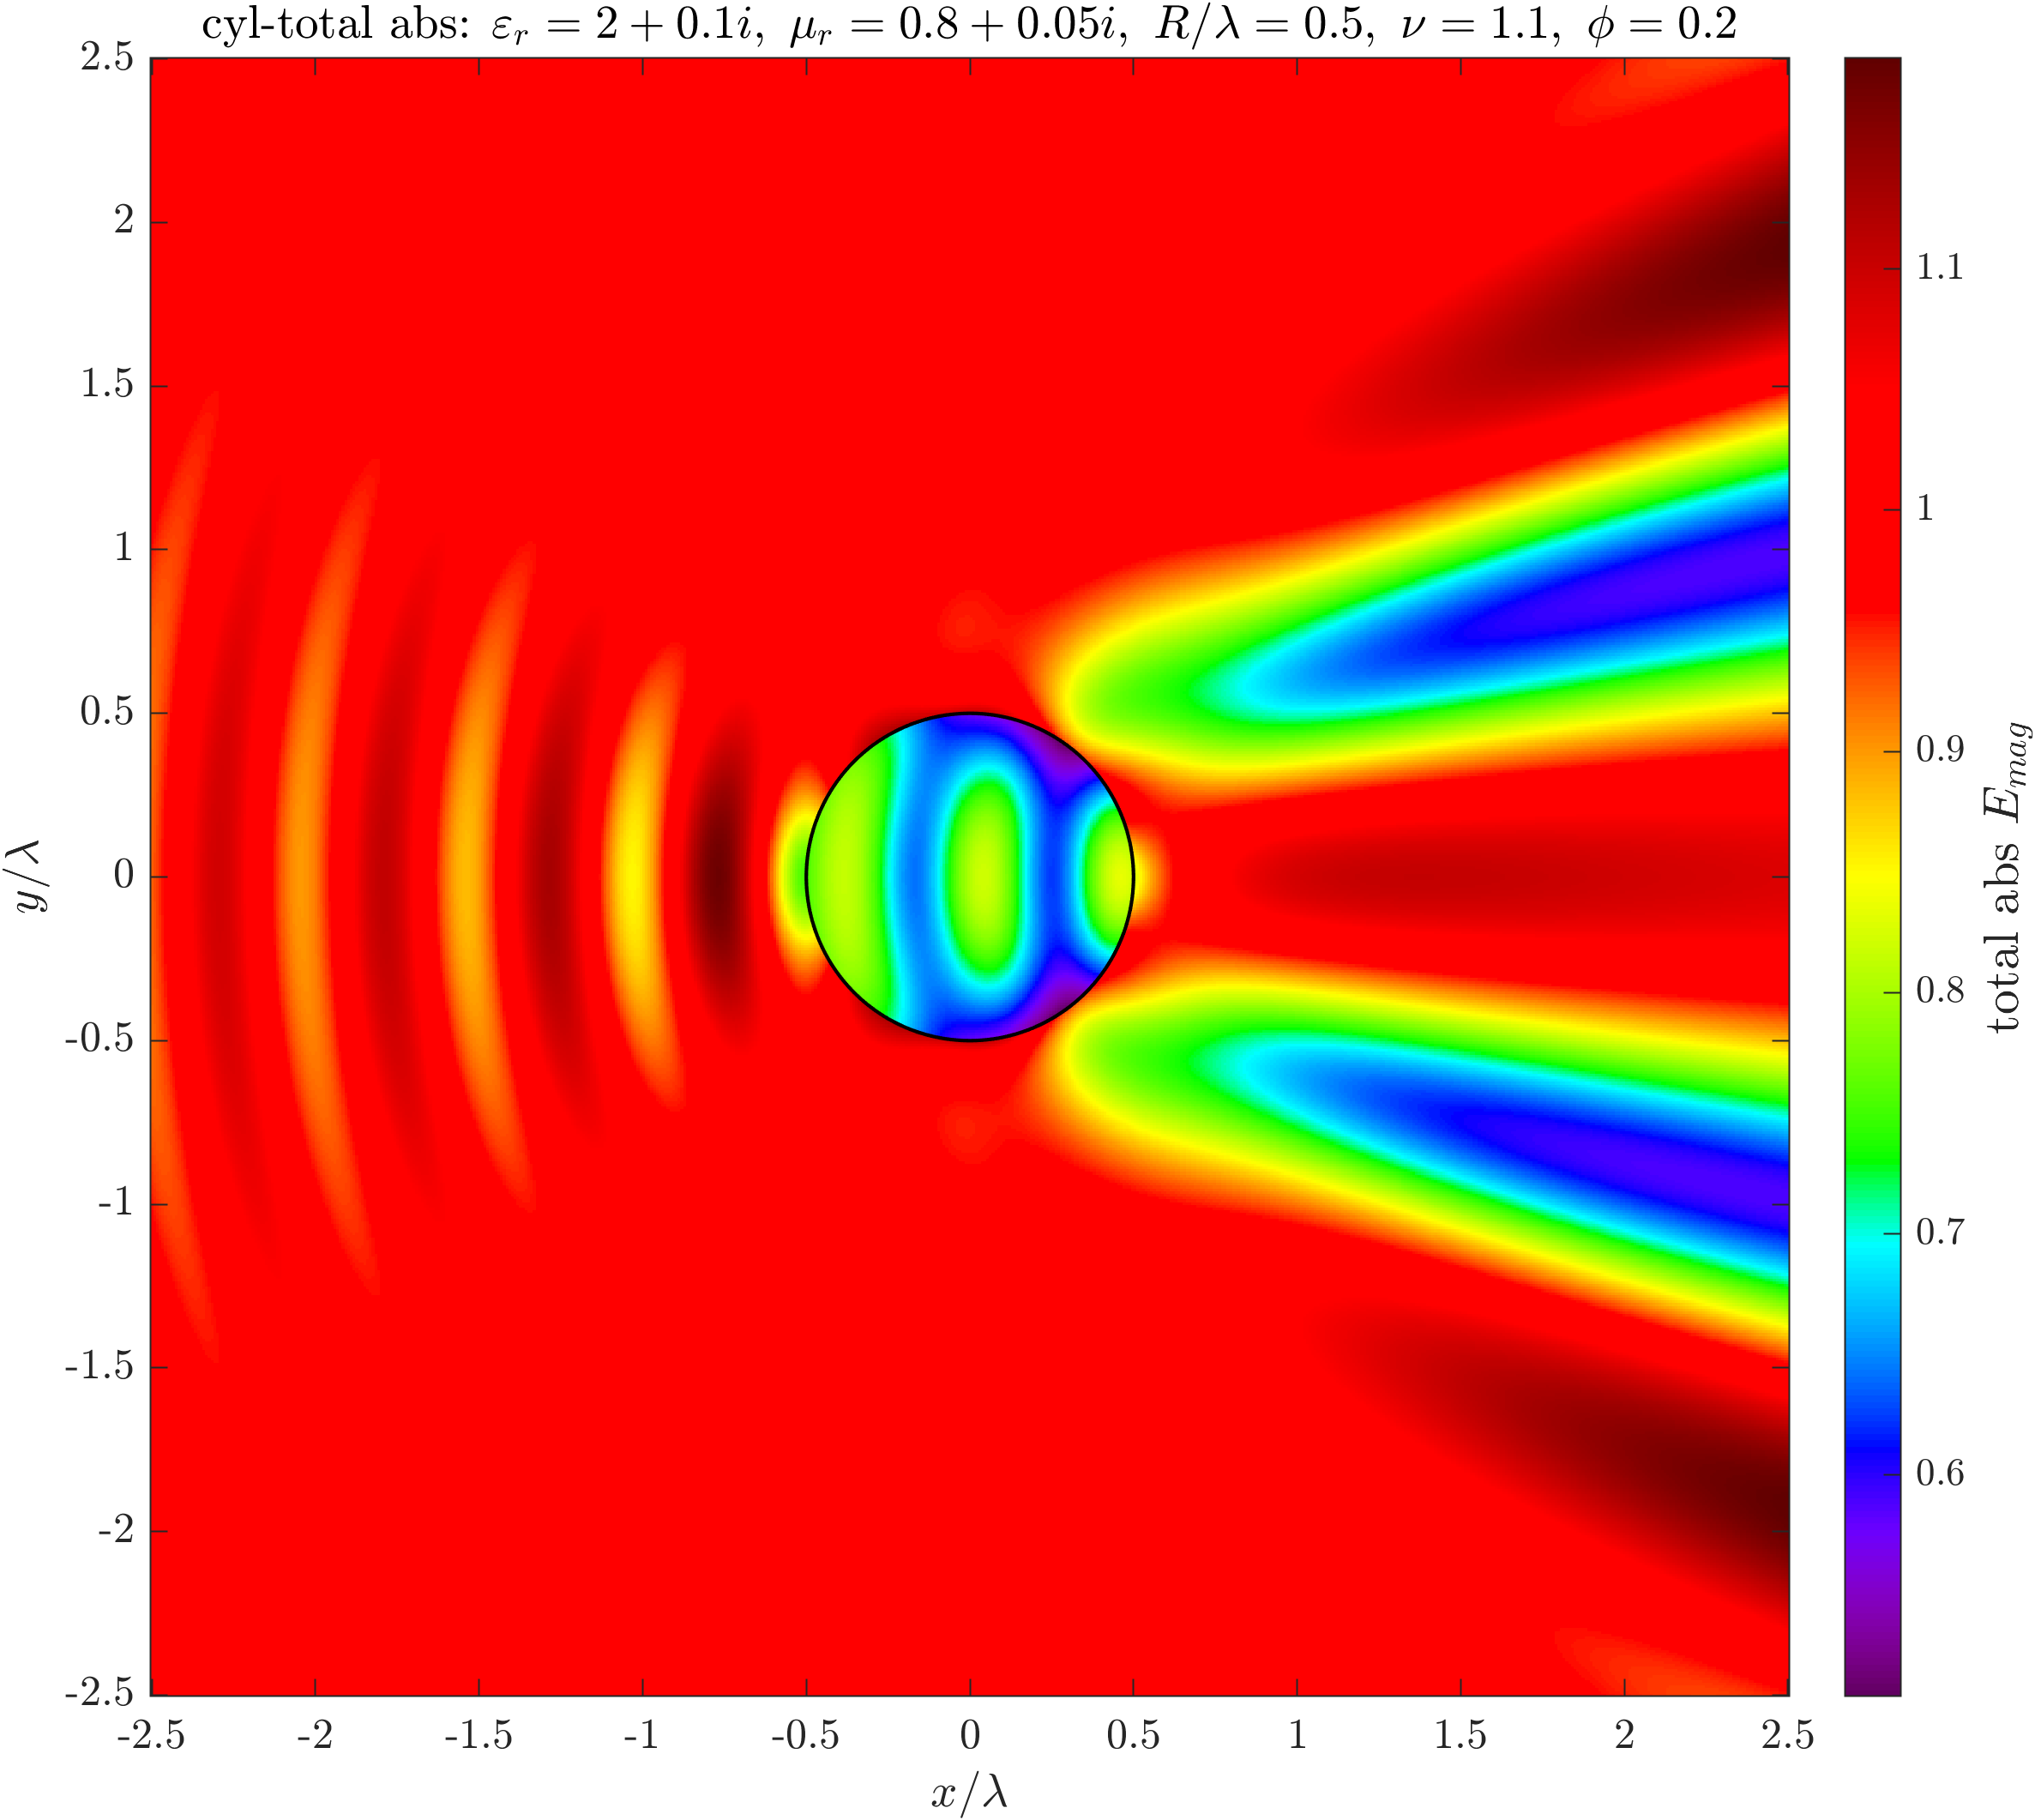
\includegraphics[width=\linewidth]{scattering_fig/lossy_small_cylinder.png}
			\caption{有损小柱}
			\label{柱体总场振幅比较图(对比有无损耗及不同半径)-有损小柱}
		\end{subfigure}
		\hfill
		% 第二个：有损大柱总场振幅
		\begin{subfigure}{0.3\textwidth}
			\centering
			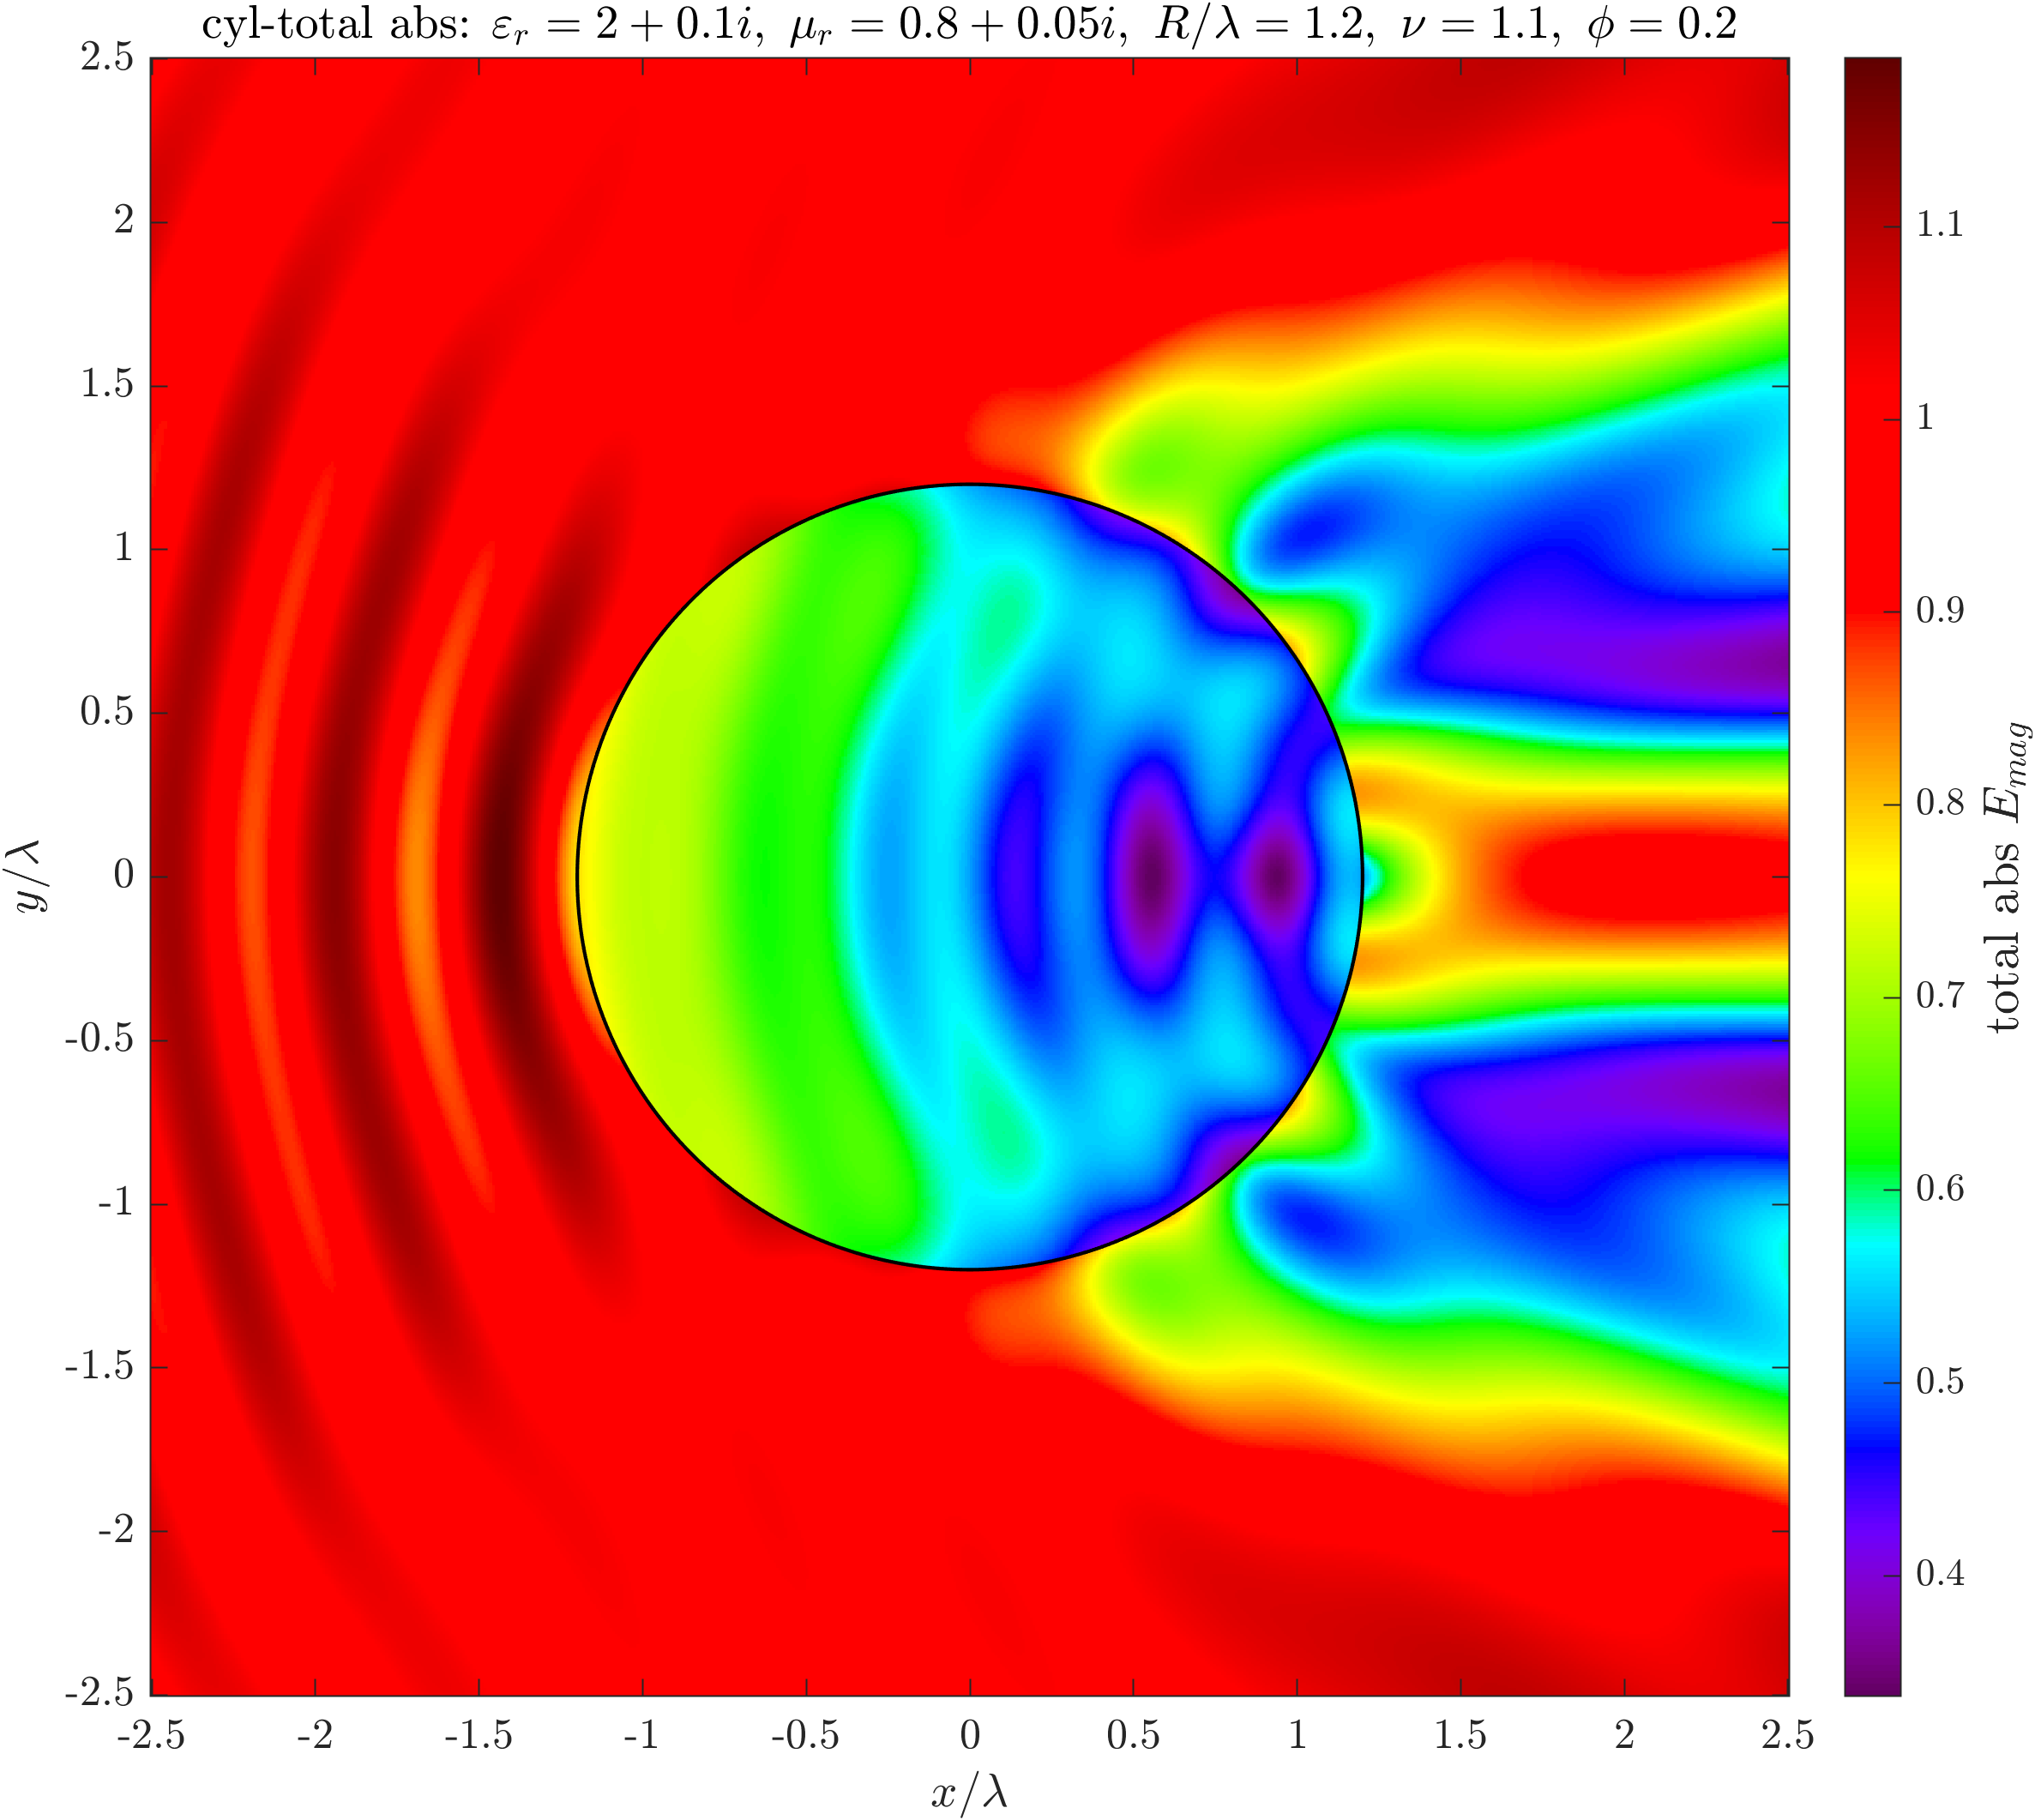
\includegraphics[width=\linewidth]{scattering_fig/lossy_large_cylinder.png}
			\caption{有损大柱}
			\label{柱体总场振幅比较图(对比有无损耗及不同半径)-有损大柱}
		\end{subfigure}
		\hfill
		% 第三个：无损大柱总场振幅
		\begin{subfigure}{0.3\textwidth}
			\centering
			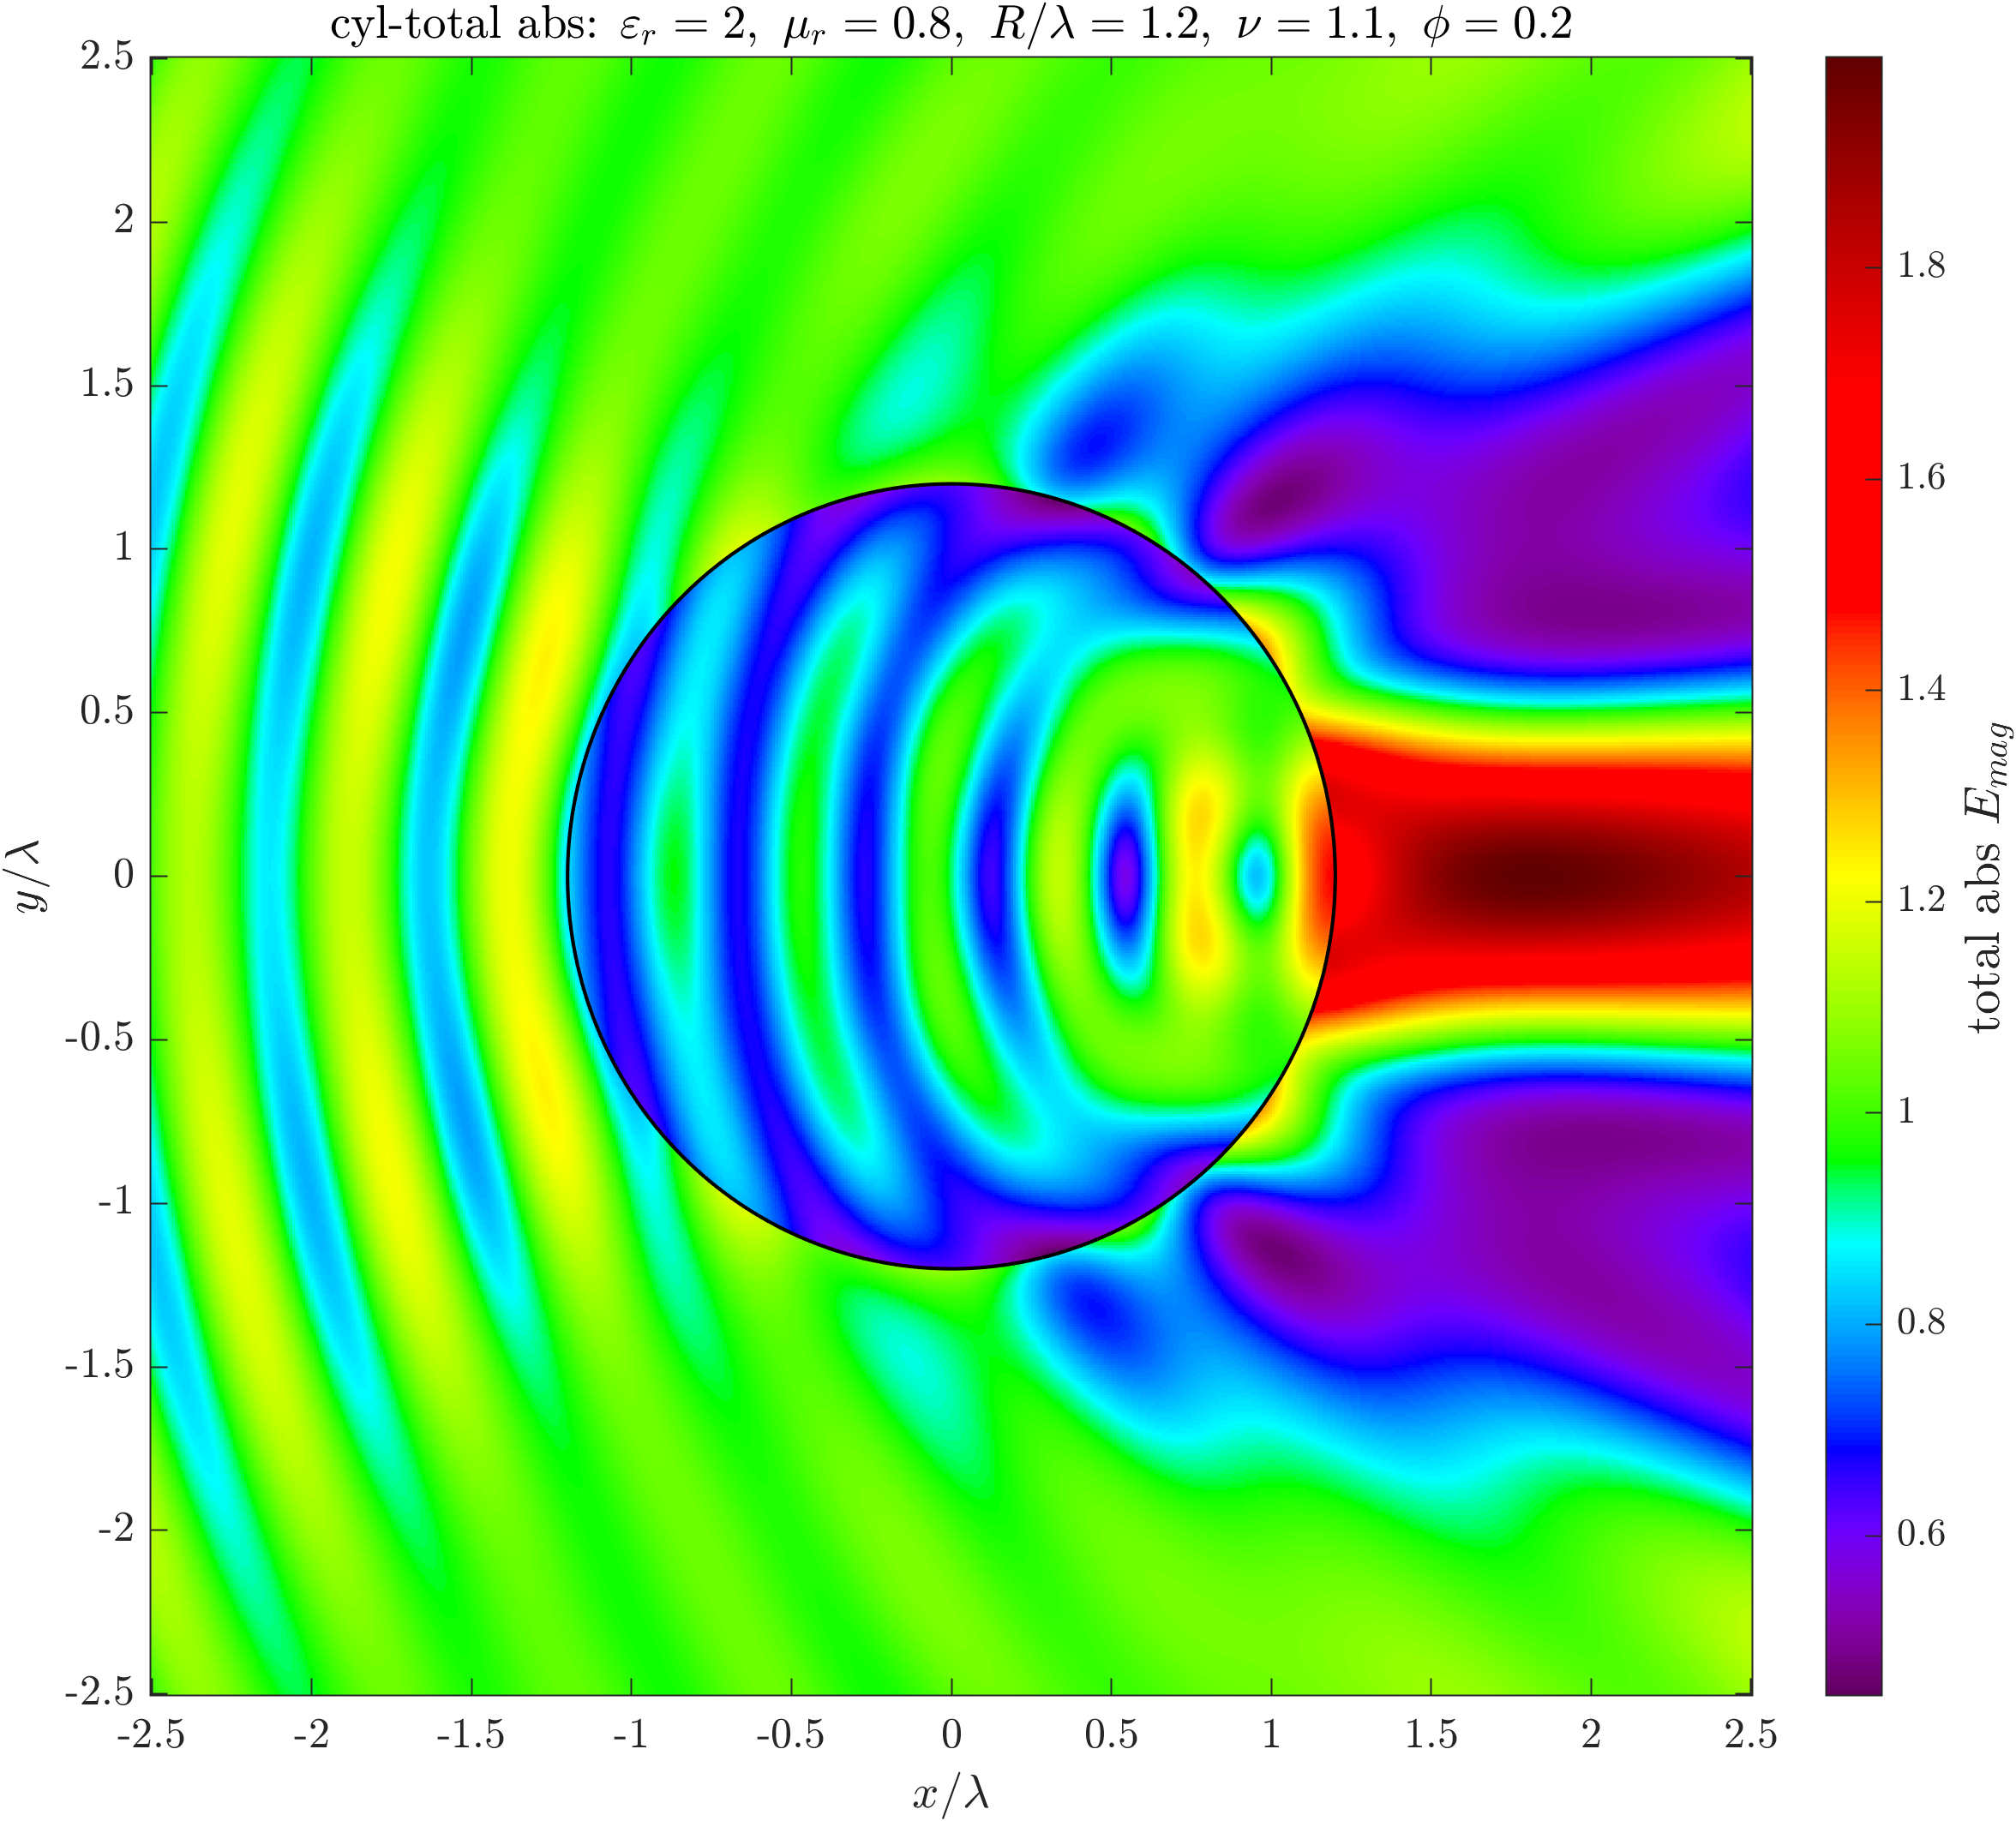
\includegraphics[width=\linewidth]{scattering_fig/lossless_large_cylinder.png}
			\caption{无损大柱}
			\label{柱体总场振幅比较图(对比有无损耗及不同半径)-无损大柱}
		\end{subfigure}

		\caption{柱体总场振幅比较图（对比有无损耗及不同半径）}
		\label{柱体总场振幅比较图(对比有无损耗及不同半径)}
		\label{fig:cylinder-total-comparison-loss}
	\end{figure}
\end{example}
